\documentclass[12pt,a4paper,oneside]{report}             % Single-side
%\documentclass[11pt,a4paper,twoside,openright]{report}  % Duplex

\usepackage{ifxetex}
\ifxetex
  \usepackage{fontspec}
\else
  \usepackage[T1]{fontenc}
  \usepackage[utf8]{inputenc}
  \usepackage{lmodern}
\fi

\usepackage[magyar]{babel} % Alapértelmezés szerint utoljára definiált nyelv lesz aktív, de később külön beállítjuk az aktív nyelvet.

\usepackage{combelow}
\usepackage{newunicodechar}

\newunicodechar{Ș}{\cb{S}}
\newunicodechar{ș}{\cb{s}}
\newunicodechar{Ț}{\cb{T}}
\newunicodechar{ț}{\cb{t}}

\usepackage{cmap}
\usepackage{amsfonts,amsmath,amssymb} % Mathematical symbols.
\usepackage[ruled,boxed,resetcount,linesnumbered]{algorithm2e} % For pseudocodes.
\def\algorithmcfname{algoritmus}
\makeatletter
\renewcommand{\fnum@algocf}{\AlCapSty{\AlCapFnt\thealgocf.\nobreakspace\algorithmcfname}}
\makeatother

\usepackage{booktabs} % For publication quality tables for LaTeX
\usepackage{graphicx}
\usepackage{sidecap}

%\usepackage{fancyhdr}
%\usepackage{lastpage}

\usepackage{anysize}
\usepackage{sectsty}
\usepackage{setspace}  % Ettol a tablazatok, abrak, labjegyzetek maradnak 1-es sorkozzel!

% For hyperlinks in the generated document. 
\usepackage{color}
\usepackage{listings} % For source code snippets.

%\usepackage[amsmath,thmmarks]{ntheorem} % Theorem-like environments.

\usepackage[hang]{caption}
\usepackage{scrextend}

\usepackage{indentfirst}
\usepackage{pdfpages}

\usepackage{xfrac}
\usepackage{eurosym}

\usepackage{fullpage} % a margokra is lehessen irni

\newcommand{\vigyazat}{\marginpar{\textcolor{red}{\emph{Vigy\'azat!}}}}

\usepackage{tikz}
\usepackage{verbatim}
\usetikzlibrary{arrows,shapes}
\usetikzlibrary{positioning}
\tikzset{main node/.style={circle,fill=blue!20,draw,minimum size=1cm,inner sep=0pt},
}

\usepackage{setspace}

\usepackage{svg}

\lstset{
  language=Python,
  basicstyle=\ttfamily,
  literate=
    {á}{{\'a}}1
    {é}{{\'e}}1
    {í}{{\'i}}1
    {ó}{{\'o}}1
    {ö}{{\"o}}1
    {ő}{{\H{o}}}1
    {ú}{{\'u}}1
    {ü}{{\"u}}1
    {ű}{{\H{u}}}1
}

\usepackage{dirtree}

%--------------------------------------------------------------------------------------
% Language configuration -- choose one
%--------------------------------------------------------------------------------------
%--------------------------------------------------------------------------------------
% Elnevezések
%--------------------------------------------------------------------------------------
\newcommand{\dolgozatnyelve}{\selectlanguage{magyar}}



\newcommand{\bsc}{Diplomadolgozat}
\newcommand{\msc}{Disszert\'aci\'os dolgozat}

\newcommand{\pelda}{Példa}
\newcommand{\definicio}{Definíció}
\newcommand{\tetel}{Tétel}

\newcommand{\bevezeto}{Bevezető}
\newcommand{\koszonetnyilvanitas}{Köszönetnyilvánítás}
\newcommand{\abrakjegyzeke}{Ábrák jegyzéke}
\newcommand{\tablazatokjegyzeke}{Táblázatok jegyzéke}
\newcommand{\irodalomjegyzek}{Irodalomjegyzék}
\newcommand{\fuggelek}{Függelék}


\newcommand{\englishParagraph}{
	\setlength{\parindent}{0em} % angol nyelvű dokumentumokban jellemző
	\setlength{\parskip}{0.5em} % angol nyelvű dokumentumokban jellemző
	\nonfrenchspacing
}

\newcommand{\hungarianParagraph}{
	\setlength{\parindent}{2em} % angol nyelvű dokumentumokban jellemző
	\setlength{\parskip}{0em}   % angol nyelvű dokumentumokban jellemző
	\frenchspacing
        \onehalfspacing
}

\newcommand{\defaultParagraph}{
	\hungarianParagraph
}
  % Beállítások magyar nyelvű dolgozathoz

%--------------------------------------------------------------------------------------
% Main variables
%--------------------------------------------------------------------------------------



% Szak alapkepzes vagy mesteri
\newcommand{\szakHU}{INFORMATIKA SZAK} % SZOFTVERFEJLESZTES
\newcommand{\szakRO}{SPECIALIZAREA INFORMATIC\v A} % SPECIALIZAREA DEZVOLTAREA APLICA\c TIILOR SOFTWARE
\newcommand{\szakEN}{COMPUTER SCIENCE SPECIALIZATION} %SOFTWARE DEVELOPMENT SPECIALIZATION


\newcommand{\dolgozattipusHU}{DIPLOMADOLGOZAT} % MESTERI DISSZERT\'ACI\'O
\newcommand{\dolgozattipusRO}{LUCRARE DE DIPLOM\v A} %TEZA DE MASTERAT
\newcommand{\dolgozattipusEN}{BACHELOR THESIS} % MASTER THESIS

\newcommand{\szerzo}{Derzsi Dániel} % Szerző neve
\newcommand{\temavezetoA}{Győrfi Ágnes} 


% Fokozatok

%Egyetemi tan\'ar/ Profesor universitar/Full Professor
%Egyetemi docens/ Conferențiar universitar/Associate professor
%Egyetemi adjunktus/Lector universitar sau Șef de lucrări /Lecturer
%Egyetemi tan\'arseg\'ed/Asistent universitar/Assistant professor


\newcommand{\temavezetoAfokozat}{Tanársegéd}% Első konzulens neve
\newcommand{\temavezetoAfokozatRo}{Asistent universitar}
\newcommand{\temavezetoAfokozatEn}{Assistant lecturer}
\newcommand{\temavezetoB}{Kátai Zoltán} % Második konzulens neve; hagyd üresen, ha egy konzulensed van.
\newcommand{\temavezetoBfokozat}{Egyetemi docens}% Első konzulens neve
\newcommand{\temavezetoBfokozatRo}{Conferențiar universitar}
\newcommand{\temavezetoBfokozatEn}{Associate professor}
\newcommand{\cimHu}{Project Raccoon - Szerződéskötések és ingatlanértékesítések korszerűsítése internetes platformon keresztül} % Cím
\newcommand{\cimRO}{Project Raccoon - Gestionarea unei platforme pentru eficientizarea finalizării de contracte și a vânzărilor de proprietăți prin intermediul internetului}
\newcommand{\cimEN}{Project Raccoon - Management of a Platform to Streamline Contract Creation and Property Sales Through the Web}
\newcommand{\ev}{2023} %az aktualis ev

%--------------------------------------------------------------------------------------
% Page layout setup
%--------------------------------------------------------------------------------------
% we need to redefine the pagestyle plain
% another possibility is to use the body of this command without \fancypagestyle
% and use \pagestyle{fancy} but in that case the special pages
% (like the ToC, the References, and the Chapter pages)remain in plane style

\usepackage{smartdiagram}
\usepackage{tikz,pgf}
\usepackage{pgfplots}

\usepackage{enumitem}
\usepackage{longtable}
\usepackage{multirow}

\usepackage{booktabs}
\usepackage{tabularx}
\usepackage{lipsum}

\pgfplotsset{width=7cm,compat=1.8}
\usetikzlibrary{matrix,calc,shapes}

\tikzset{
	treenode/.style = {shape=rectangle, rounded corners, draw, anchor=center, text width=5em, align=center, top color=white, bottom color=blue!20,inner sep=1ex},
	decision/.style = {treenode, diamond, inner sep=0pt},
	root/.style = {treenode, font=\Large, bottom color=red!30},
	env/.style = {treenode, font=\ttfamily\normalsize},
	finish/.style = {root, bottom color=green!40},
	dummy/.style = {circle,draw}
}

\setcounter{secnumdepth}{0}
\sectionfont{\large\upshape\bfseries}
\setcounter{secnumdepth}{2}

\sloppy % Margón túllógó sorok tiltása.
\widowpenalty=10000 \clubpenalty=10000 %A fattyú- és árvasorok elkerülése
\def\hyph{-\penalty0\hskip0pt\relax} % Kötőjeles szavak elválasztásának engedélyezése

%--------------------------------------------------------------------------------------
% Setup hyperref package
%--------------------------------------------------------------------------------------
\usepackage{xcolor}
\definecolor{bluecite}{HTML}{0875b7}
\usepackage[unicode=true,
	bookmarksopen={true},
	pdffitwindow=true, 
	colorlinks=true, 
	linkcolor=bluecite, 
	citecolor=bluecite, 
	urlcolor=bluecite, 
	hyperfootnotes=false, 
	pdfstartview={FitH},
	pdfpagemode= UseNone]{hyperref}

%--------------------------------------------------------------------------------------
% Set up listings
%--------------------------------------------------------------------------------------

\definecolor{codegreen}{rgb}{0,0.6,0}
\definecolor{codegray}{rgb}{0.5,0.5,0.5}
\definecolor{codepurple}{rgb}{0.58,0,0.82}
\definecolor{backcolour}{rgb}{0.95,0.95,0.92}

\definecolor{lightgray}{rgb}{0.95,0.95,0.95}
\definecolor{darkgreen}{RGB}{3,125,80}
\lstset{frame=tb,
	language=Matlab,
	aboveskip=3mm,
	belowskip=3mm,
	showstringspaces=false,
	columns=flexible,
	basicstyle={\small\ttfamily},
	numbers=none,
	numberstyle=\tiny\color{gray},
	keywordstyle=\color{blue},
	commentstyle=\color{codegreen},
	%stringstyle=\color{mauve},
	breaklines=true, breakatwhitespace=true, tabsize=3,
	backgroundcolor=\color{lightgray}, } \def\lstlistingname{k\'odr\'eszlet}

%--------------------------------------------------------------------------------------
% Set up theorem-like environments
%--------------------------------------------------------------------------------------
% Using ntheorem package -- see http://www.math.washington.edu/tex-archive/macros/latex/contrib/ntheorem/ntheorem.pdf
%\swapnumbers
%\theoremstyle{plain}
%\theoremseparator{.}
\newtheorem{example}{\pelda}[section]

%\theoremseparator{.}
%\theoremprework{\bigskip\hrule\medskip}
%\theorempostwork{\hrule\bigskip}
%\theorembodyfont{\upshape}
%\theoremsymbol{{\large \ensuremath{\centerdot}}}
\newtheorem{definition}{\definicio}[section]

%\theoremseparator{.}
%\theoremprework{\bigskip\hrule\medskip}
%\theorempostwork{\hrule\bigskip}
\newtheorem{theorem}{\tetel}[section]

\newtheorem{conclusion}{Következtetés}[section]

%--------------------------------------------------------------------------------------
% Some new commands and declarations
%--------------------------------------------------------------------------------------
\newcommand{\code}[1]{{\upshape\ttfamily\scriptsize\indent #1}}
\newcommand{\doi}[1]{DOI: \href{http://dx.doi.org/\detokenize{#1}}{\raggedright{\texttt{\detokenize{#1}}}}} % A hivatkozások közt így könnyebb DOI-t megadni.

\DeclareMathOperator*{\argmax}{arg\,max}
%\DeclareMathOperator*[1]{\floor}{arg\,max}
\DeclareMathOperator{\sign}{sgn}
\DeclareMathOperator{\rot}{rot}

%--------------------------------------------------------------------------------------
% Setup captions
%--------------------------------------------------------------------------------------

\captionsetup[figure]{
	width=.75\textwidth,
	aboveskip=10pt}
\renewcommand{\captionlabelfont}{\bf}
%\renewcommand{\captionfont}{\footnotesize\it}

%--------------------------------------------------------------------------------------
% Redefine reference style
%--------------------------------------------------------------------------------------
\newcommand{\figref}[1]{\ref{fig:#1}.}
\renewcommand{\eqref}[1]{(\ref{eq:#1})}
\newcommand{\listref}[1]{\ref{listing:#1}.}
\newcommand{\sectref}[1]{\ref{sect:#1}}
\newcommand{\tabref}[1]{\ref{tab:#1}.}

% -----
% Table
% -----
\newenvironment{requirementstable}
{\begin{longtable}{|p{0.25\textwidth}|p{0.70\textwidth}|}}
		{\hline\end{longtable}}

\newcommand{\requirementtitle}[1]{
	\hline
	\multirow{2}{*}[-0.25cm]{\textbf{#1}}
}

\newcommand{\requirementtitlewordwrap}[1]{
	\hline
	\multirow{2}{*}[-0.25cm]{\parbox{4cm}{\centering\textbf{#1}}}
}

\newcommand{\requirementslist}[1]{
	\setlist[enumerate]{leftmargin=0.8cm, rightmargin=0.5cm, topsep=0cm, parsep=0cm}
	\begin{enumerate}
		#1
	\end{enumerate}
}

\lstdefinelanguage{TS}{
	keywords={break, case, catch, continue, debugger, default, delete, do, else, finally, for, function, if, in, instanceof, new, return, switch, this, throw, try, typeof, var, void, while, with},
	morecomment=[l]{//},
	morecomment=[s]{/*}{*/},
	morestring=[b]',
	morestring=[b]",
	sensitive=true
}

\newcommand{\hiddensubsection}[1]{
	\subsection*{#1}
	\stepcounter{subsection}
}

\newcommand{\hiddennumberedsubsection}[1]{
	\subsection{#1}
	\stepcounter{subsection}
}




%--------------------------------------------------------------------------------------
% Table of contents and the main text
%--------------------------------------------------------------------------------------
\begin{document}
	
% CIMOLDALAK
%~~~~~~~~~~~~~~~~~~~~~~~~~~~~~~~~~~~~~~~~~~~~~~~~~~~~~~~~~~~~~~~~~~~~~~~~~~~~~~~~~~~~~~
	%--------------------------------------------------------------------------------------
%	A magyar cimoldal
%--------------------------------------------------------------------------------------
\begin{titlepage}
	\begin{center}
	
		\large{\bfseries SAPIENTIA ERDÉLYI MAGYAR TUDOMÁNYEGYETEM} \\
		\large{\bfseries MAROSVÁSÁRHELYI KAR,} \\
		\large{\bfseries \szakHU} \\[1.75cm]
			\begin{center}
			
\includegraphics[scale=2]{images/sapientia-hu}
		\end{center}
		\vspace{0.4cm}
		\Large{\Large  \cimHu}\\[0.8cm]
		\vspace{0.2cm}
		\textsc{\Large \bfseries \dolgozattipusHU}\\[2.5cm]
		
		{
			\large
		
			\renewcommand{\arraystretch}{0.85}
			\begin{tabular}{cc}
				 \makebox[6.5cm]{Témavezető:} & \makebox[6.5cm]{Végzős hallgató:} \\ \noalign{\smallskip}
				 \makebox[6.5cm]{\temavezetoA, \temavezetoAfokozat} & \makebox[6.5cm]{\szerzo} \\ {\temavezetoB, \temavezetoBfokozat}
			\end{tabular}
		}
		
		\vfill
		{\large \bfseries \ev}
	\end{center}
\end{titlepage}
	%--------------------------------------------------------------------------------------
%	The title page RO
%--------------------------------------------------------------------------------------

\begin{titlepage}
	\begin{center}
	
		\large{\bfseries UNIVERSITATEA SAPIENTIA DIN CLUJ-NAPOCA} \\
		\large{\bfseries FACULTATEA DE ȘTIINȚE TEHNICE ȘI UMANISTE,} \\
		
		\large{\bfseries \szakRO} \\[1.25cm]
		
			\begin{center}
			
\includegraphics[scale=2]{images/sapientia-ro}
		\end{center}
		
		\vspace{0.4cm}
		
	
		
		\Large{\Large \cimRO}\\[0.5cm]
		\vspace{0.25cm}
		\textsc{\Large \bfseries \dolgozattipusRO}\\[2.5cm]
		
		{
			\large
		
			\renewcommand{\arraystretch}{0.85}
			\begin{tabular}{cc}
				 \makebox[6.5cm]{Coordonator științific:} & \makebox[6.5cm]{Absolvent:} \\ \noalign{\smallskip}
				 \makebox[6.5cm]{\temavezetoA, \temavezetoAfokozatRo} & \makebox[6.5cm]{\szerzo} \\
				 {\temavezetoB, \temavezetoBfokozatRo}
			\end{tabular}
		}
		
		\vfill
		{\large \bfseries \ev}
	\end{center}
\end{titlepage}
	%--------------------------------------------------------------------------------------
%	The title page EN
%--------------------------------------------------------------------------------------

\begin{titlepage}
	\begin{center}
	
		\large{\bfseries SAPIENTIA HUNGARIAN UNIVERSITY OF TRANSYLVANIA} \\
		\large{\bfseries FACULTY OF TECHNICAL AND HUMAN SCIENCES} \\
		\large{\bfseries \szakEN} \\[1.25cm]
		
			\begin{center}
			
\includegraphics[scale=2]{images/sapientia-en}
		\end{center}
		\vspace{0.4cm}
		\Large{\Large  \cimEN}\\[0.5cm]
		\vspace{0.5cm}
		\textsc{\Large \bfseries \dolgozattipusEN}\\[2.5cm]
		
		{
			\large
	
			\renewcommand{\arraystretch}{0.85}
			\begin{tabular}{cc}
				 \makebox[6.5cm]{Scientific advisor:} & \makebox[6.5cm]{Student:} \\ \noalign{\smallskip}
				 \makebox[6.5cm]{\temavezetoA, \temavezetoAfokozatEn} & \makebox[6.5cm]{\szerzo} \\
				 {\temavezetoB, \temavezetoBfokozatEn}
			\end{tabular}
		}
		
		\vfill
		{\large \bfseries \ev}
	\end{center}
\end{titlepage}
	
	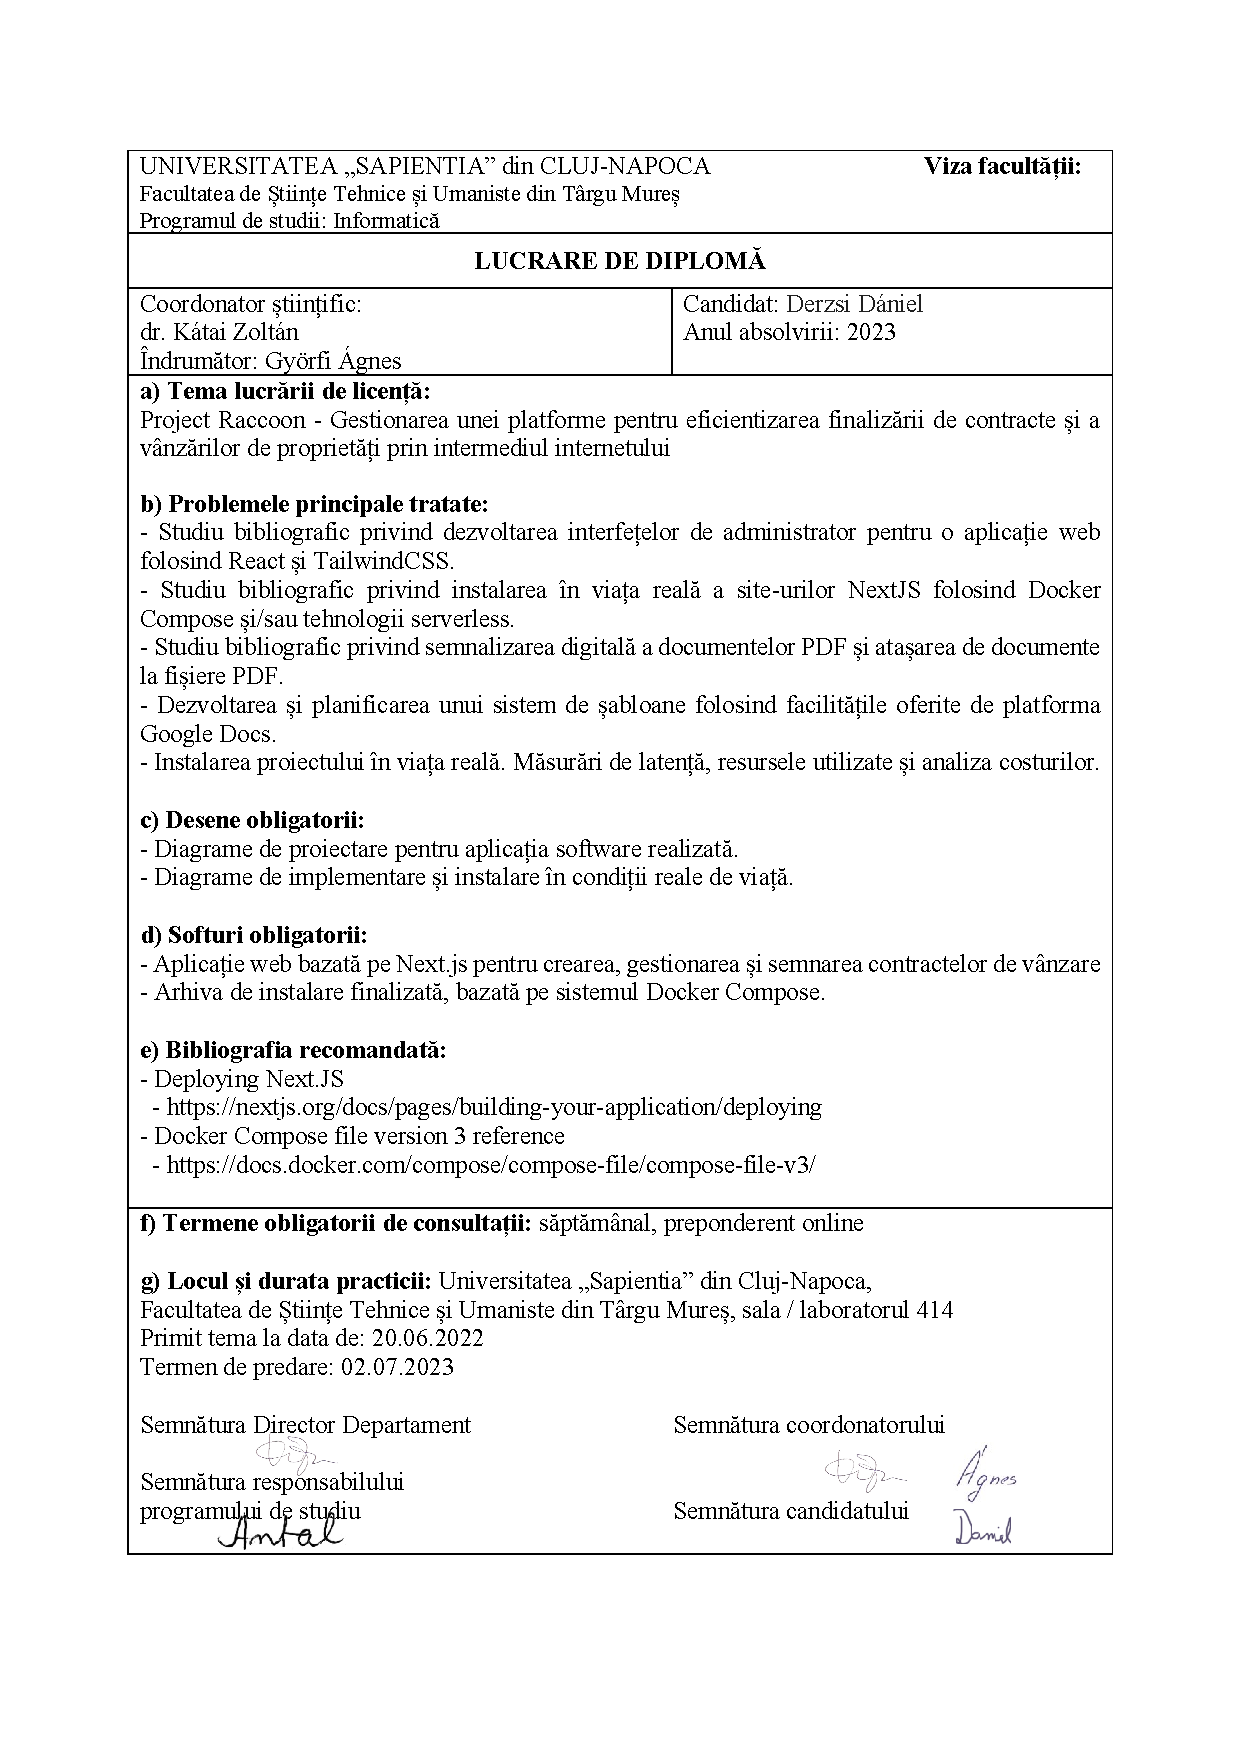
\includepdf[pages={1}]{embed/fisa.pdf}
	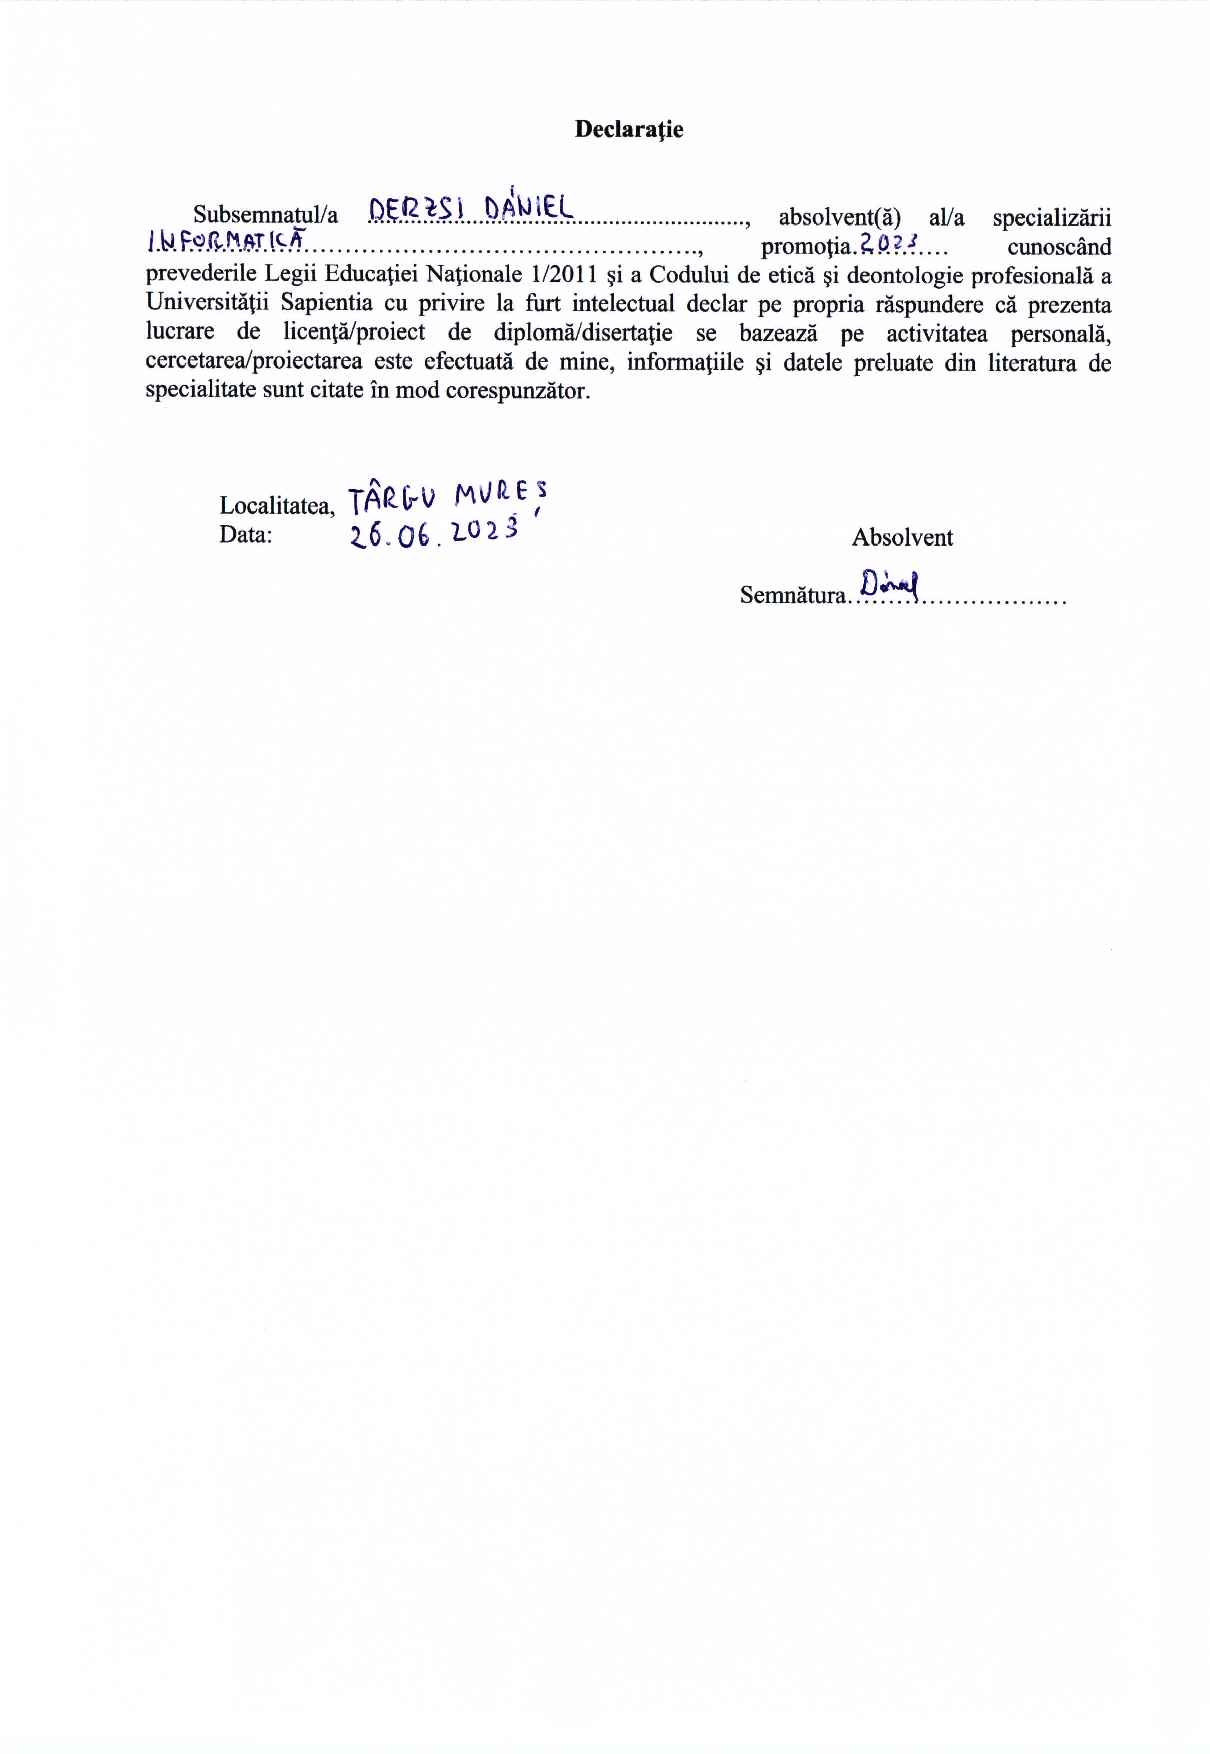
\includepdf[pages={1}]{embed/declaratie.pdf}

        \pagenumbering{gobble}

\selectlanguage{magyar}
\hungarianParagraph

%----------------------------------------------------------------------------
% Abstract in Hungarian
%----------------------------------------------------------------------------

\chapter*{Kivonat}
\begin{spacing}{1}

A mai rohanó világban az ingatlanügyletekben részt vevő magánszemélyek és vállalkozások gyakran jelentős kihívásokkal szembesülnek az ingatlan- és tulajdonadásvételi szerződések elkészítésekor. Ezen szerződések létrehozása az ingatlanügyletek szerves részét képzi, összetett jogi szabályok böngészésével és aprólékos dokumentáció írását köteleztetve. Szükség van egy olyan intuitív eszköz kitalálására, amely enyhíti ezeket a bonyolult folyamatok végigjárását, és megkönnyíti a jogszabályoknak megfelelő, pontos szerződések létrehozását.

Dolgozatom témája kettős. Először is, meg kívánom teremteni egy olyan online platform alapjait, amely lehetővé teszi a szerződések automatikus létrehozását a biztonságos ingatlanértékesítések megkönnyítése érdekében. Ez magában foglalja a szükséges szoftverarchitektúra megtervezését, egy könnyen kezelhető adminisztrációs felület létrehozását, valamint PDF dokumentumok szó szerinti generálását és kitöltését az adminisztrátorok által létrehozott sablonok segítségével. Másodszor, szándékomban áll dokumentálni a végső kitelepítés különböző szakaszait (és lehetőségeit), valós körülmények között mérve.

A javasolt weboldal átfogó platformként szolgál, barátságos felületet kínálva a felhasználóknak a saját igényeikre szabott, jogilag teljes bizonyító erejű szerződések létrehozására. Azáltal, hogy nincs szükség kiterjedt jogi ismeretekre vagy költséges ügyvédek fizetésére, a szerződések létrehozásához szükséges idő és erőfeszítés jelentősen csökken.

Összehasonlításképpen, világszerte hasonló szoftvermegoldásokat vezetett be számos kormány az adásvételi szerződésekkel kapcsolatos kihívások kezelésére. Ezeket a kormányok által támogatott törekvéseket azonban gyakran jelentősen hátráltatják a meggondolatlan tervezési döntéseik és az eredendő homályosságuk. Platformunk célja, hogy a felhasználók számára olyan egyedi leegyszerűsített élményt nyújtson, amely felülmúlja a meglévő kormányzati kezdeményezéseket.

A szakdolgozat elején a javasolt szoftveres megoldás létrehozásához alkalmazott technológiákat tárgyaljuk. Ezt követően leírjuk, hogy mit fog a szoftver szolgáltatni, és hogy milyen teljesítményt várunk el tőle egy szoftverkövetelményspecifikáció részeként. A lehetséges szoftverarchitektúra és telepítési bemutatását követően részletesen bemutatjuk a platform leendő felhasználói felületét. Végezetül bemutatunk néhány mérést a szoftverarchitektúra tervezési szakaszában hozott döntéseink racionalizálása érdekében.

\vskip 0.5cm

\textbf{Kulcsszavak}: \textit{Tulajdonszerződések}, \textit{Dokumentumsablonok}, \textit{PDF dokumentumgenerálás}, \textit{Dockeres kitelepítés}, \textit{Serverless technológiák}.
\end{spacing}
\vfill
\selectlanguage{romanian}

%----------------------------------------------------------------------------
% Abstract in Romanian
%----------------------------------------------------------------------------
\chapter*{Rezumat}
\begin{spacing}{1}

În ziua de azi, persoanele fizice și juridice angajate în tranzacții imobiliare se confruntă adesea cu provocări semnificative atunci când redactează contracte de vânzare de proprietăți. Crearea acestor contracte de vânzare a proprietății este partea integrală a tranzacțiilor imobiliare, implicând legalități complexe și necesitatea unei documentații meticuloasă. Există o nevoie pentru un instrument intuitiv care să atenueze aceste complexități și să faciliteze crearea unor contracte precise și conforme cu legea.

Scopul tezei mele este dublu. În primul rând, intenționez să creez bazele unei platforme online care să permită crearea automată de contracte pentru a facilita vânzarea sigură a proprietăților. Aceasta include planificarea unei arhitecturii software necesare, crearea unei interfețe de administrare ușor de utilizat, precum și generarea și completarea propriu-zisă a documentelor PDF, folosind șabloanele create de către administratori. În al doilea rând, intenționez să documentez diferitele etape (și posibilități) ale instalării finale, măsurate în condiții reale.

Site-ul web propus servește ca o platformă cuprinzătoare, oferind utilizatorilor o interfață prietenoasă pentru a genera contracte obligatorii din punct de vedere juridic, adaptate la cerințele lor specifice. Prin eliminarea necesității unor cunoștințe juridice extinse sau a asistenței unor avocați costisitori, timpul și efortul necesar pentru a crea un contract sunt mult reduse.

Comparativ, guvernele din întreaga lume au implementat soluții software asemănătoare pentru a aborda provocările asociate cu contractele de vânzare de proprietăți. Cu toate acestea, aceste eforturi susținute de guverne sunt adesea dezavantajate în mod semnificativ de obscuritatea lor percepută. Această platformă își propune să ofere utilizatorilor o experiență unică și simplificată, care depășește inițiativele guvernamentale existente.

La începutul tezei vom discuta diferitele tehnologii utilizate pentru a crea soluția software propusă. Ulterior, vom descrie ceea ce va face software-ul și cum se așteaptă să funcționeze ca parte a unei specificații a cerințelor software (\textit{SRS}). O interfață de utilizator prospectivă pentru platformă va fi detaliată în urma propunerii unei arhitecturi software. În cele din urmă, vor fi prezentate câteva măsurători pentru a raționaliza deciziile luate în timpul etapelor de planificare a arhitecturii software.

\vskip 0.5cm

\textbf{Cuvinte cheie}: \textit{Contracte de proprietate}, \textit{Șabloane}, \textit{Generarea de documente PDF}, \textit{Instalare folosind Docker}, \textit{Tehnologii serverless}.
\end{spacing}
\vfill
\selectlanguage{english}
%\englishParagraph

%----------------------------------------------------------------------------
% Abstract in English
%----------------------------------------------------------------------------
\chapter*{Abstract}
\begin{spacing}{1}

In today's fast-paced world, individuals and businesses engaged in real estate transactions often encounter significant challenges when drafting property sale contracts. The creation of these property sale contracts is an integral part of real estate transactions, involving complex legalities and meticulous documentation. There is a pressing need for an intuitive tool that can alleviate these complexities and facilitate the creation of accurate and legally compliant contracts.

The aim of my thesis is two-fold. Firstly, I intend to create the basis of an online platform to allow the automatic creation of contracts to facilitate secure property sales. This includes the creation and planification of the necessary software architecture, the creation of an easy to use administration interface, as well as the verbatim generation and filling out of PDF documents using templates created by the administrators. Secondly, I intend to document the various stages (and possibilities) of the final deployment, measured within real-world conditions.

The proposed website serves as a comprehensive platform, offering users a friendly interface to generate legally binding contracts tailored to their specific requirements. By eliminating the need for extensive legal knowledge or the assistance of costly attorneys, the time and effort required to create a contract is greatly reduced.

Comparatively, governments worldwide have implemented similar software solutions to address the challenges associated with property sale contracts. However, these government-backed endeavours are often significantly handicapped by their perceived obscurity and their convoluted design choices. This platform aims to provide users with a unique and simplified experience that surpasses existing government initiatives.

In the beginning of the thesis we will discuss the various technologies employed to create the proposed software solution. Afterwards, we will describe what the software will do and how it will be expected to perform as part of a Software Requirements Specification. A prospective user interface for the platform will be detailed following the proposal of a potential software architecture and deployment layout. Finally, some measurements will be presented to rationalize the decisions taken during the planning stages of the software architecture.

\vskip 0.5cm

\textbf{Keywords}: \textit{Property contracts}, \textit{Document templates}, \textit{PDF document generation}, \textit{Docker deployment}, \textit{Serverless technologies}.
\end{spacing}
\vfill
\dolgozatnyelve
\defaultParagraph
 
% Tartalomjegyzek
%~~~~~~~~~~~~~~~~~~~~~~~~~~~~~~~~~~~~~~~~~~~~~~~~~~~~~~~~~~~~~~~~~~~~~~~~~~~~~~~~~~~~~~
	\pagenumbering{arabic}
	\setcounter{page}{9}
	\tableofcontents\vfill

% A diplomadolgozat lenyegi resze
%~~~~~~~~~~~~~~~~~~~~~~~~~~~~~~~~~~~~~~~~~~~~~~~~~~~~~~~~~~~~~~~~~~~~~~~~~~~~~~~~~~~~~~

	%----------------------------------------------------------------------------
\chapter{Bevezető}%\addcontentsline{toc}{chapter}{Bevezető}
%----------------------------------------------------------------------------

Az évek során a technológia robbanásszerű fejlődésen ment keresztül, számos területen átalakította életünket. Számtalan ügy, amelyet azelőtt személyesen kellett lebonyolítani, átkerült az online világba, az internetre. Ez az online ügyintézési folyamat a modern technológia által kínált előnyök és lehetőségek következménye, és gyökeresen megváltoztatta mindennapi életünk dinamikáját. 

Az interneten történő ügyintézés számos előnnyel és kényelemmel jár a mai ember számára. Az egyik legnyilvánvalóbb az idő megtakarítása. Ezelőtt, ha valamilyen ügyet szerettünk volna intézni, a megfelelő hivatalt személyesen kellett felkeresnünk, amely órákba vagy egyes esetekben akár napokba is telhetett. Nem kell időpontot előzetesen személyesen egyeztetni, nem kell hosszú sorokat kivárni. Nem szükséges szabadnapot kivenni a munkahelyről az ügyek elintézése végett, illetve bármikor, akár este is végezhetjük ügyeink intézését, a technológia révén most már otthonunk kényelméből tudjuk ügyes-bajos dolgainkat intézni, vagy bárhonnan, ahol internet-hozzáférésünk van - legyen ez akár a mindennapi tömegközkekedés során mobiltelefonunk segítségével. Egyszerűen bejelentkezünk az illetékes weboldalra, kitöltjük a szükséges űrlapokat vagy elvégezzük a szükséges tranzakciókat, és néhány kattintással elintézzük az ügyet. Könnyen belátható tehát, hogy az online ügyintézés igénybevételével sokkal nagyobb szabadságfokot és rugalmat élvezhetünk saját időbeosztásunk tekintetében. 

Ezzel párhuzamosan nemcsak számunkra, hanem az intézmények és vállalatok számára is hasznosak ezen internetes platformok: csökkenthetik az adminisztrációs terheket, a munkaerőigényt (hiszen az ügyfelek maguk tudják elvégezni ügyeiket), gyorsabb kiszolgálást tesz lehetővé a különböző folyamatok automatizálásával, az adatok online tárolásával és kezelésével. 

Az online ügyintézés rohamos terjedése a technológiai fejlődés mértékét tükrözi, és az életünk szerves részévé vált. Az internet lehetőséget ad számunkra, hogy gyorsan és hatékonyan intézzük az ügyeinket, miközben megtakarítjuk az értékes időnket és növeljük a kényelmünket.

Néhány ország annyira élenjár a technológiai fejlődésben, hogy állampolgáraik képesek majdnem minden ügyeiket az internet segítségével intézni. Sajnos kevés ország tartozik jelenleg ezen országok közé. Magyarország vagy Románia esetében számos ügyet csak személyesen lehet továbbra is lebonyolítani. Ilyen kategóriába tartoznak az adásvételi szerződések. Amennyiben az említett országokban szeretnénk eladni vagy épp venni ingóságot vagy épp ingatlant, számos jogi lépéseken kell keresztül menni, amelyek esetenként napokat is felölelhetnek. Nem vitatott tehát, hogy egy hosszadalmas és stresszes procedúráról van szó. 
 
Az üzleti világban a szerződések elengedhetetlenek az adásvételi folyamatok lebonyolításához és a jogi biztonság fenntartásához. Azonban a hagyományos módszerekkel járó papír alapú szerződéskötés és az azt követő adminisztráció gyakran időigényes és bonyolult folyamatot jelentett. Azonban most, a Project Raccoon platform bemutatkozásával, egy teljesen új megközelítés jelentkezik az adásvételi szerződések kezelésében.

A Project Raccoon egy forradalmi platformot kínál, amely lehetővé teszi minden szerződéses fél számára, hogy egyszerűen és hatékonyan kezelje és aláírja az adásvételi szerződéseket. Ez a platform megszabadítja őket az időrabló és körülményes adminisztratív feladatoktól, és lehetővé teszi a jogi formulációk gyors és könnyed elvégzését.

A Raccoon platformja új dimenziót ad az adásvételi szerződések generálásához és kezeléséhez. Az alkalmazás egyszerűen használható felhasználói felülete és intuitív navigációja révén minden fél - akár eladók, vevők, vállalkozások vagy magánszemélyek - egyszerűen és hatékonyan tudja kitölteni és aláírni a szerződéseket.

A platform úttörő módon automatizálja a szerződések létrehozását a kormány által kiadott hivatalos sablonok alapján. Ez jelentősen megkönnyíti a szerződéskötés folyamatát, hiszen a feleknek már nincs szükségük szakértői jogi ismeretekre vagy ügyvédi segítségre ahhoz, hogy létrehozzanak egy pontos és jogilag érvényes szerződést. A Raccoon platformja gondoskodik arról, hogy minden szükséges jogi információ és kitöltendő mező rendelkezésre álljon, így a felhasználók egyszerűen csak kitölthetik az adott részeket, és a platform automatikusan generálja a szerződést.

Az adásvételi szerződések digitalizálása és azok kezelésének egyszerűsítése egyértelműen egy hatalmas előrelépést jelent a Project Raccoon platformja által kínált innovatív megoldással. A Raccoon platformja segítségével a szerződések elkészítése és aláírása könnyebbé válik, a folyamat pedig gyorsabbá és hatékonyabbá válik minden érintett számára.
	\chapter{Elméleti megalapozás}\label{chapter1}

\section{Piacelemzés}

A dolgozat ezen részében megvizsgáljuk a konténerizációs világ adta
lehetőségeket, és bemutatjuk a Zebrafish által kitöltött piaci rést. A
felhőplatformokra való nagyfokú összpontosítás miatt a konténerizáció világa az
elmúlt években jelentős növekedésnek indult, mivel a vállalatok egyre inkább
felismerik a konténerek előnyeit: a hordozhatóságot, a skálázhatóságot és az
erőforrás-hatékonyságot.

\subsection{Virtuális gépek: VMWare vSphere / ESXi}

\begin{figure}[h]
        \centering
        \includesvg[scale=0.75]{images/survey/vmwarevsphere.svg}
        \caption{A VMWare vSphere logója}
        \label{vsphere}
\end{figure}

Mielőtt elkezdenénk beszélni a konténerekről, meg kell értenünk a virtualizáció
jelenlegi helyzetét. A virtualizáció már régóta létezik, és széles körben
elterjedt az iparágban. Az egyik legnépszerűbb virtualizációs platform a
\ref{vsphere} ábrán látható VMWare vSphere, azon belül pedig a VMware ESXi. A
VMWare ESXi egy hipervizor: lehetővé teszi több virtuális gép futtatását
egyetlen fizikai szervergépen. Más szavakkal élve: lehetőséget biztosít több
operációs rendszer futtatására egyetlen gépen.

A VMWare ESXi azonban rendelkezik bizonyos korlátozásokkal. Ez egy
szabadalmaztatott szoftver, ami azt jelenti, hogy nem nyílt forráskódú és nem
szabadon használható. Ha ez nem elég, 2024 elején a VMWare megszüntette az ESXi
ingyenes verzióját, ami azt jelenti, hogy a felhasználóknak mostantól licenszt
kell fizetniük a használatáért. \cite{vmware2024eol} Ez sok frusztrációhoz vezetett a közösségben,
mivel sokan személyes projektekhez vagy a virtualizáció megismeréséhez az
ingyenes verziót használta.

\begin{figure}[h]
        \centering
        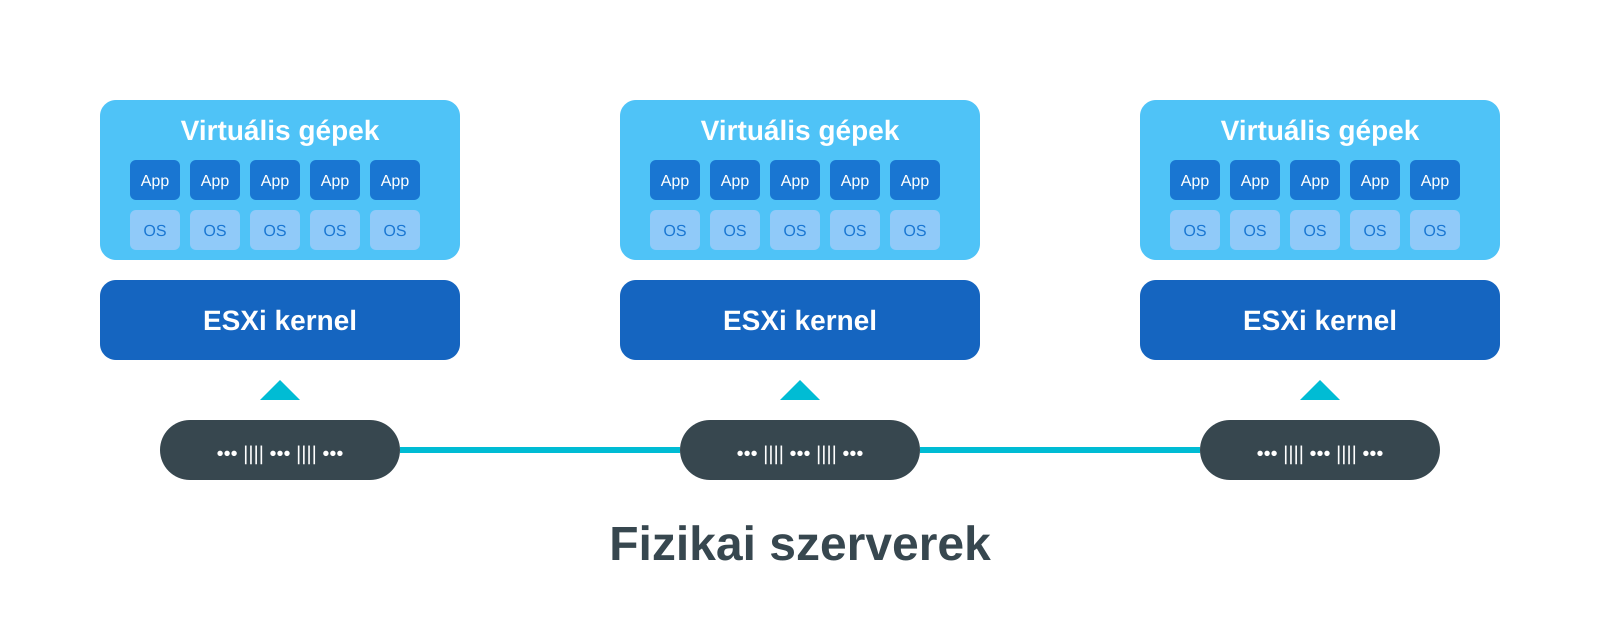
\includegraphics[scale=0.75]{images/survey/esxiexplanation.png}
        \caption{A VMWare ESXi működési elve}
        \label{esxi}
\end{figure}

Az \ref{esxi} ábrán látható a VMWare ESXi működése. A felhasználók telepíthetik
az ESXi-t a fizikai gépre, majd létrehozhatnak és kezelhetnek virtuális gépeket
a vSphere kliens segítségével. A virtuális gépek teljesen elszigetelt
környezetek, amelyek saját operációs rendszerrel rendelkeznek. Az egyes
operációs rendszereken elkülönített alkalmazások futnak.

Az ESXi operációsrendszer-független. Közel áll nagyon egy hagyományos operációs
rendszerhez, mivel saját kernellel és felhasználói felülettel rendelkezik. Ez a
komplexitás azonban nem száll át a virtualizált operációs rendszerek
rendszergazdáira. Ugyanakkor nem olyan rugalmas, mint más virtualizációs
megoldások, például a KVM vagy a Xen, mivel csak bizonyos
hardverkonfigurációkat támogat.

\subsection{KVM}

A KVM rövidítése a \textit{Kernel-based Virtual Machine}-nek, ami egy nyílt
forráskódú virtualizációs technológia, amely a Linux kernelbe van integrálva. A
KVM lehetővé teszi, hogy egy Linux rendszeren hipervizorként futva több
virtuális gép futtatható legyen egyetlen fizikai gépen.

A VMware ESXi-hez képest a KVM nyílt forráskódú. Rugalmasabb, hiszen a
felhasználók a szokásos Linux parancsokkal hozhatnak létre és kezelhetnek
virtuális gépeket. A KVM emellett pehelysúlyúbb is, mivel a meglévő Linux
kernelt használja a virtualizációs képességek biztosításához, ahelyett, hogy
külön hypervisort igényelne.

A VMware ESXi-t leginkább vállalati környezetben telepítenek, míg a KVM-et
inkább felhőkörnyezetekben használják, vagy olyan fejlesztők, akik virtuális
gépeket szeretnének futtatni saját hardverükön. A Linux hardvertámogatását
kihasználva számos hardverkonfigurációt támogat. Emellett ingyenes, ami miatt
számos tárhelyszolgáltató kínál KVM-alapú virtuális privát szervereket (VPS)
versenyképes áron. \cite{xenkvm}

Azonban mind a VMWare ESXi, mind a KVM rendelkezik korlátokkal. Elsősorban
virtuális gépek futtatására tervezték őket, amelyek erőforrás-igényesek
lehetnek, és nem feltétlenül a leghatékonyabb módja a könnyű alkalmazások vagy
microservice-ek futtatásának.\footnote{Meglepő módon még a konténerizáció is
        visszanyúl néha a virtualizációhoz, mivel néhány konténer-futtatórendszer, mint
        például a \textit{Firecracker}, biztonsági okokból KVM-et használ a konténerek
        virtuális gépen történő futtatására.} Itt jön képbe a konténerizáció.

\subsection{Konténerizáció: Docker és Docker Desktop}

\begin{figure}[!h]
        \centering
        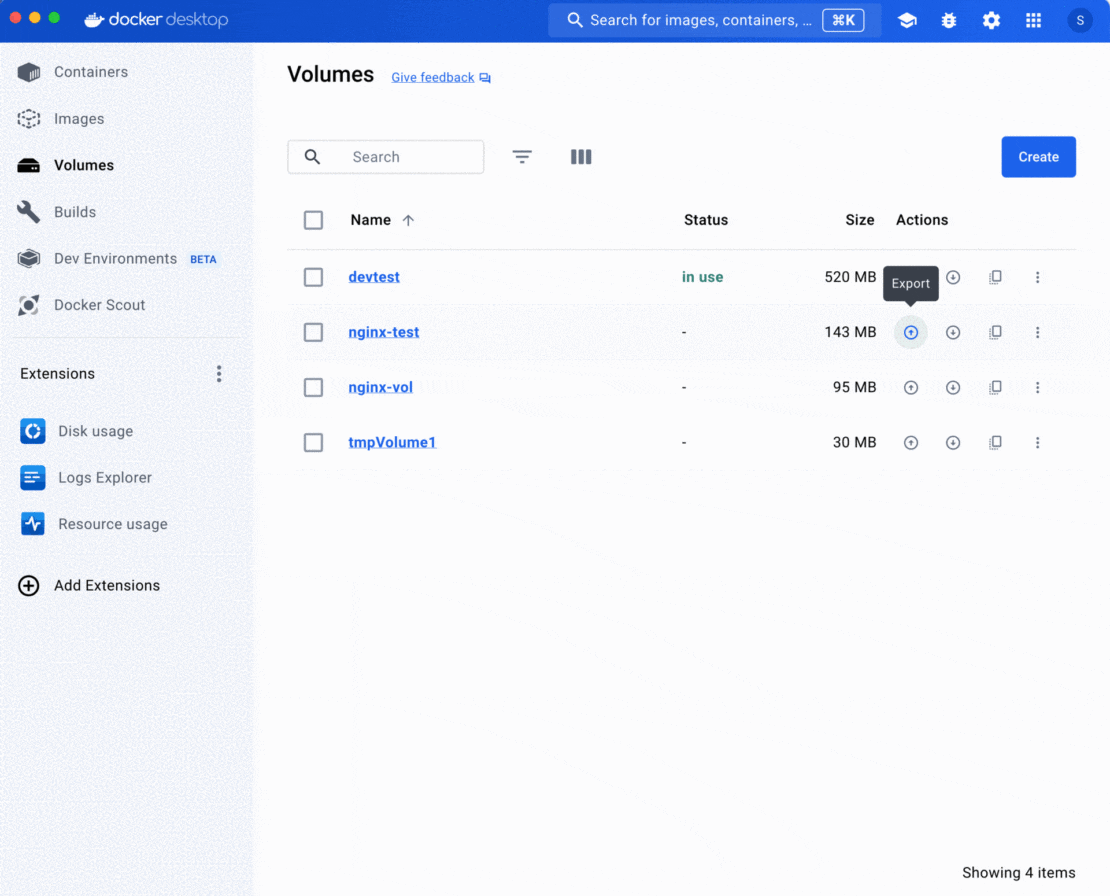
\includegraphics[scale=0.4]{images/survey/dockerdesktop.png}
        \caption{A Docker Desktop kinézete}
        \label{docker}
\end{figure}

A Docker (lásd \ref{docker}. ábra) egy részben nyílt forráskódú platform, amely
lehetővé teszi alkalmazások elkülönített konténerekben történő telepítését,
skálázását és kezelését. A Docker már a konténerizáció szinonimája. A
konténerek gyakorlatilag futó Docker image-ek, amelyek mögött egy virtuális
fájlrendszer és a hozzájuk tartozó folyamatok állnak. A Docker image-ek önálló,
hordozható környezetet biztosítanak, amelyek tartalmazzák az alkalmazást,
valamint annak minden függőségét, beleértve az operációs rendszer könyvtárait
és szükséges könyvtárakat is.

Bár a konténerek közösen használják a gazdagép operációs rendszerének kernelét
a Docker környezeten belül, biztonsági szempontból hasonló védelmet nyújtanak,
mint a hagyományos virtuális gépek \cite{containersec}. Az alkalmazás
függőségeivel egyött egyetlen egységbe zárva futnak, így minimalizálódnak az
esetleges fájlrendszerbeli konfliktusok, és biztosítható a környezet pontos
reprodukálhatósága. Mivel a konténerek mögött nem áll hagyományos operációs
rendszer, kevesebb erőforrást igényelnek, mint a hagyományos virtuális gépek,
valamint gyorsabban indíthatók. A hardvert hatékonyabban ki tudjuk használni,
és gyorsabban skálázhatjuk az alkalmazásainkat.

A Dockert és a Docker Compose-t széles körben alkalmazzuk mind a fejlesztési,
mind az éles környezetünkben. A Docker Compose segítségével definiált
szolgáltatásokat gyakran különálló projektekbe szervezzük, így ezek a rendszer
más Compose-projektjeitől függetlenül, atomi módon indíthatók, újraindíthatók
vagy leállíthatók: ezáltal a karbantartás rendkívül egyszerűvé válik.

Manapság a Docker Engine egy nyílt-forráskódú konténer-platformon alapszik, a
Moby projekten. A Moby projekt célja, hogy egy moduláris, szabadon bővíthető
alapot biztosítson konténeres rendszerek építéséhez, amelyből a Docker saját
megoldása is építkezik. Ez a projekt a Docker projektből született, amely
eredetileg egy monolitikus alkalmazás volt. A Moby projekt nyílt forráskódú, hogy a közösség felkarolásával tudják fejleszteni. \cite{ghosh2020docker} A Docker CLI-on, a Docker Swarm-on és a Docker Scout-on kívül a
Docker cég további termékei, mint például a Docker Desktop, zárt forráskódúák és
külön licenszelemeket tartalmaznak. \cite{dockerproducts}

\subsection{BSD Jails}

A FreeBSD-ből származó BSD Jail mechanizmus egy könnyű, operációs rendszer
szintű virtualizációs technológia, amely megelőzte a Dockerhez hasonló
konténerek széles körű elterjedését. A jail ugyan nem egy teljes értékű
virtuális gép, de biztonságos, elszigetelt környezeteket (``jail'') hoz létre
egyetlen FreeBSD operációs rendszeren belül. Minden jail saját hostnévvel,
IP-címmel és külön fájlrendszerfával rendelkezik, így a benne futó folyamatok
számára önálló rendszernek tűnik.

A BSD Jails a konténerizáció egyik legkorábbi formája, amely a teljes hardveres
virtualizáció többletköltségei nélkül kínál folyamat-, fájlrendszer- és
hálózati izolációt. Úttörő szerepük ellenére nem értek el olyan széles körű
elterjedést, mint a későbbi konténertechnológiák, például a Docker, amely
hatalmas népszerűségre tett szert. Ez egyrészt technikai paradoxon, mivel
Linuxon a konténerizáció gyakran több, egymástól eltérő kernelfunkció
kombinálásával valósul meg (például a cgroups az erőforrás-kezeléshez és a
namespaces az elszigeteléshez), míg a BSD Jails egy integráltabb és egységesebb
megoldást kínál magában a FreeBSD kernelben. Végül a Docker győzött a könnyű
használhatóságával, az ökoszisztémájával és - ami talán a legfontosabb - a maga
köré épített közösségével.

\subsection{Podman}

\begin{figure}[!h]
        \centering
        \includesvg[scale=1.5]{images/survey/podmanlogo.svg}
        \caption{A Podman logója}
        \label{podman}
\end{figure}

A Podman (\ref{podman}. ábra) egy nyílt forráskódú, daemon nélküli
konténerkezelő eszköz. A Dockerhez hasonlóan a Podman is lehetővé teszi a
konténerek építését, futtatását és kezelését, azonban jelentős különbséggel:
nem igényel háttérben futó daemon folyamatot mint a Docker Engine. Ez a daemon
nélküli architektúra növeli a biztonságot, mivel a konténerek közvetlenül a
felhasználó folyamataiként futnak, elkerülve a root jogosultságú daemonnal járó
potenciális kockázatokat, ami a Docker esetében a legtöbb biztonsági aggály
forrása. A daemon, mint központi vezérlőforrás is megszűnik. A Docker esetében
a rendszer teljes kompromittálódásához vezethet, ha egy támadó hozzáfér a
Docker daemonhoz. A Podman esetében nincs ilyen veszély.

A Podman kiemelkedő tulajdonsága a \textit{rootless konténerek} támogatása, ami
azt jelenti, hogy a felhasználók root jogosultság nélkül is futtathatnak
konténereket. Ez tovább javítja a biztonságot. A Podman emellett kompatibilis a
Docker CLI-val, így a Docker felhasználók könnyedén átállhatnak rá, mivel a
legtöbb parancs azonos. Támogatja a Podokat is, amelyek lehetővé teszik több
konténer egyetlen egységként történő kezelését, ami különösen hasznos a
Kubernetes-kompatibilis munkafolyamatokhoz.

A Podman azonban nem mentes a kihívásoktól. Bár úgy tervezték, hogy a Docker
helyettesítésére szolgáljon, a Docker egyes funkciói nem támogatottak teljes
mértékben a Podmanban. A Podman például nem rendelkezik teljes körű Compose
implementációval, ami nehezítheti a több konténerrel rendelkező alkalmazások
kitelepítését. Van egy kísérlet arra, hogy áthidalják ezt Podman Compose
projekttel, de ez nem olyan kiforrt, mint a Docker Compose, és a gyakorlatban
meglehetősen könnyen hibát dob. \cite{ezeobi2024investigation}

\subsection{Containerd}

A \textit{containerd} egy olyan alapvető konténer-futtató daemon, amelyre
összetettebb konténer-orchestrációs platformok építhetők. A konténerek
futtatásához és kezeléséhez az abszolút minimumkövetelményeket biztosítja, de
nem kínál magas szintű képességeket vagy felhasználóbarát felületeket a
közvetlen interakcióhoz. Parancssori interfésze, az `ctr` elsősorban fejlesztők
és rendszerintegrátorok számára készült, hogy hozzáférjenek a
\textit{containerd} alacsony szintű belső részeihez, és nem javasolt a magas
szintű felhasználók számára.

A felhasználóbarát Docker CLI és az alacsony szintű containerd közötti szakadék
áthidalására olyan projektek jelentek meg, mint a \textit{nerdctl}. A
\textit{nerdctl} célja, hogy Docker-kompatibilis CLI-t biztosítson a
\textit{containerd} számára. A Compose implementációja azonban több problémával
is küzd, többek között helytelen zárási mechanizmusokkal, a multi-Compose
projekt támogatásának hiányával és a függőségek túl agresszív kezelésével.
Például két Compose parancsot nem lehet egyszerre futtatni a \textit{nerdctl}
használatával, mivel az a teljes Compose környezetet zárolja, és megakadályozza
több Compose parancs végrehajtását, amíg az első be nem fejeződik. Ez
alkalmatlanná teszi a programot az éles környezetben való használatra.

A többszörös Compose projektek csak megoldásokon keresztül támogatottak. Ha
például két olyan Compose-projekt van, amelyet egyszerre kell futtatni, akkor
azokat meghatározott sorrendben kell futtatni, ami bonyodalmakhoz vezethet. Nem
tudja automatikusan kitalálni a Compose projektek közötti függőségeket.
Emellett a \textit{nerdctl} függőségkezelése túlságosan agresszív, ami azt
jelenti, hogy megpróbálja újraindítani egy szolgáltatás függőségeit akkor is,
ha nem szükséges az újraindítás. Ez irreleváns szolgáltatások szükségtelen
leállásához vezet.

Azt is fontos megjegyezni, hogy a széles körben népszerű konténerplatform, a
Docker a \textit{containerd}-et használja a színfalak mögött a konténer
futtatórendszereként. Régebbi Kubernetes-verziók is a \textit{containerd}-t
használták a konténerek futtatására, de az újabb verziók már a \textit{CRI-O}
konténer-futtatót használják, amely a Kubernetes számára optimalizált futtató.

\subsection{Firecracker}

\begin{figure}[!h]
        \centering
        
\includegraphics[scale=0.12]{images/survey/firecracker.png}
        \caption{A Firecracker logója}
        \label{firecracker}
\end{figure}

A Firecracker (\ref{firecracker}. ábra) a konténer ökoszisztéma legújabb tagja. A Firecracker célja, hogy a konténerek gyors indítási idejét és alacsony erőforrás-felhasználását a virtuális gépek (VM-ek) által biztosított erős elszigeteltséggel kombinálja. Ehhez a KVM ökoszisztémáját használja, amely segítségével pehelysúlyú virtuális gépeket, úgynevezett microVM-eket hoz létre, amelyek minimális többletköltséggel futtathatók egy gazdaszámítógépen.

Egyetlen fizikai gépen több száz mikroVM futhat párhuzamosan, mindegyik saját kernel-lel és minimális rendszerrel. Ezek a mikroVM-ek gyorsan, akár 125 ms alatt elindíthatók, és mindössze néhány megabájt memóriát igényelnek \cite{agache2020firecracker}. A Firecracker minimalista megközelítése révén csak a legszükségesebb eszközöket és interfészeket tartalmazza, csökkentve a támadási felületet és növelve a biztonságot. Mivel Rust nyelven íródott, a Rust memóriabiztonsági garanciáit is kihasználja, ami megelőzi a biztonsági réshez vezető gyakori programozási hibákat.

Másrészt, mivel a virtio eszközökön keresztül kommunikál, nem olyan rugalmas, mint más konténer-futtatórendszerek. A Firecracker microVM-ek nem oszthatják meg a host fájlrendszerét, ami azt jelenti, hogy minden microVM-nek saját block device-okat és fájlrendszerképet kell készítenie. Ez megnehezíti az integrációt például a Zebrafish-sel, amelynek szigorú követelményei vannak az operációs rendszer által biztosított fájlrendszer használatára, ami lehetővé teszi az erős adatkonzisztencia és az automatikus adattükrözés/mentési politika alkalmazását. A Firecracker továbbá nem tud kommunikálni a hoszt eszközökkel, ami azt jelenti, hogy a Firecracker platformon nem lehetne gyorsított gépi tanulási munkaterheket, például fényképek osztályozását futtatni, mivel a hoszt gép GPU-ját nem lehetne elérni.

\subsection{Kubernetes}

\begin{figure}[!h]
        \centering
        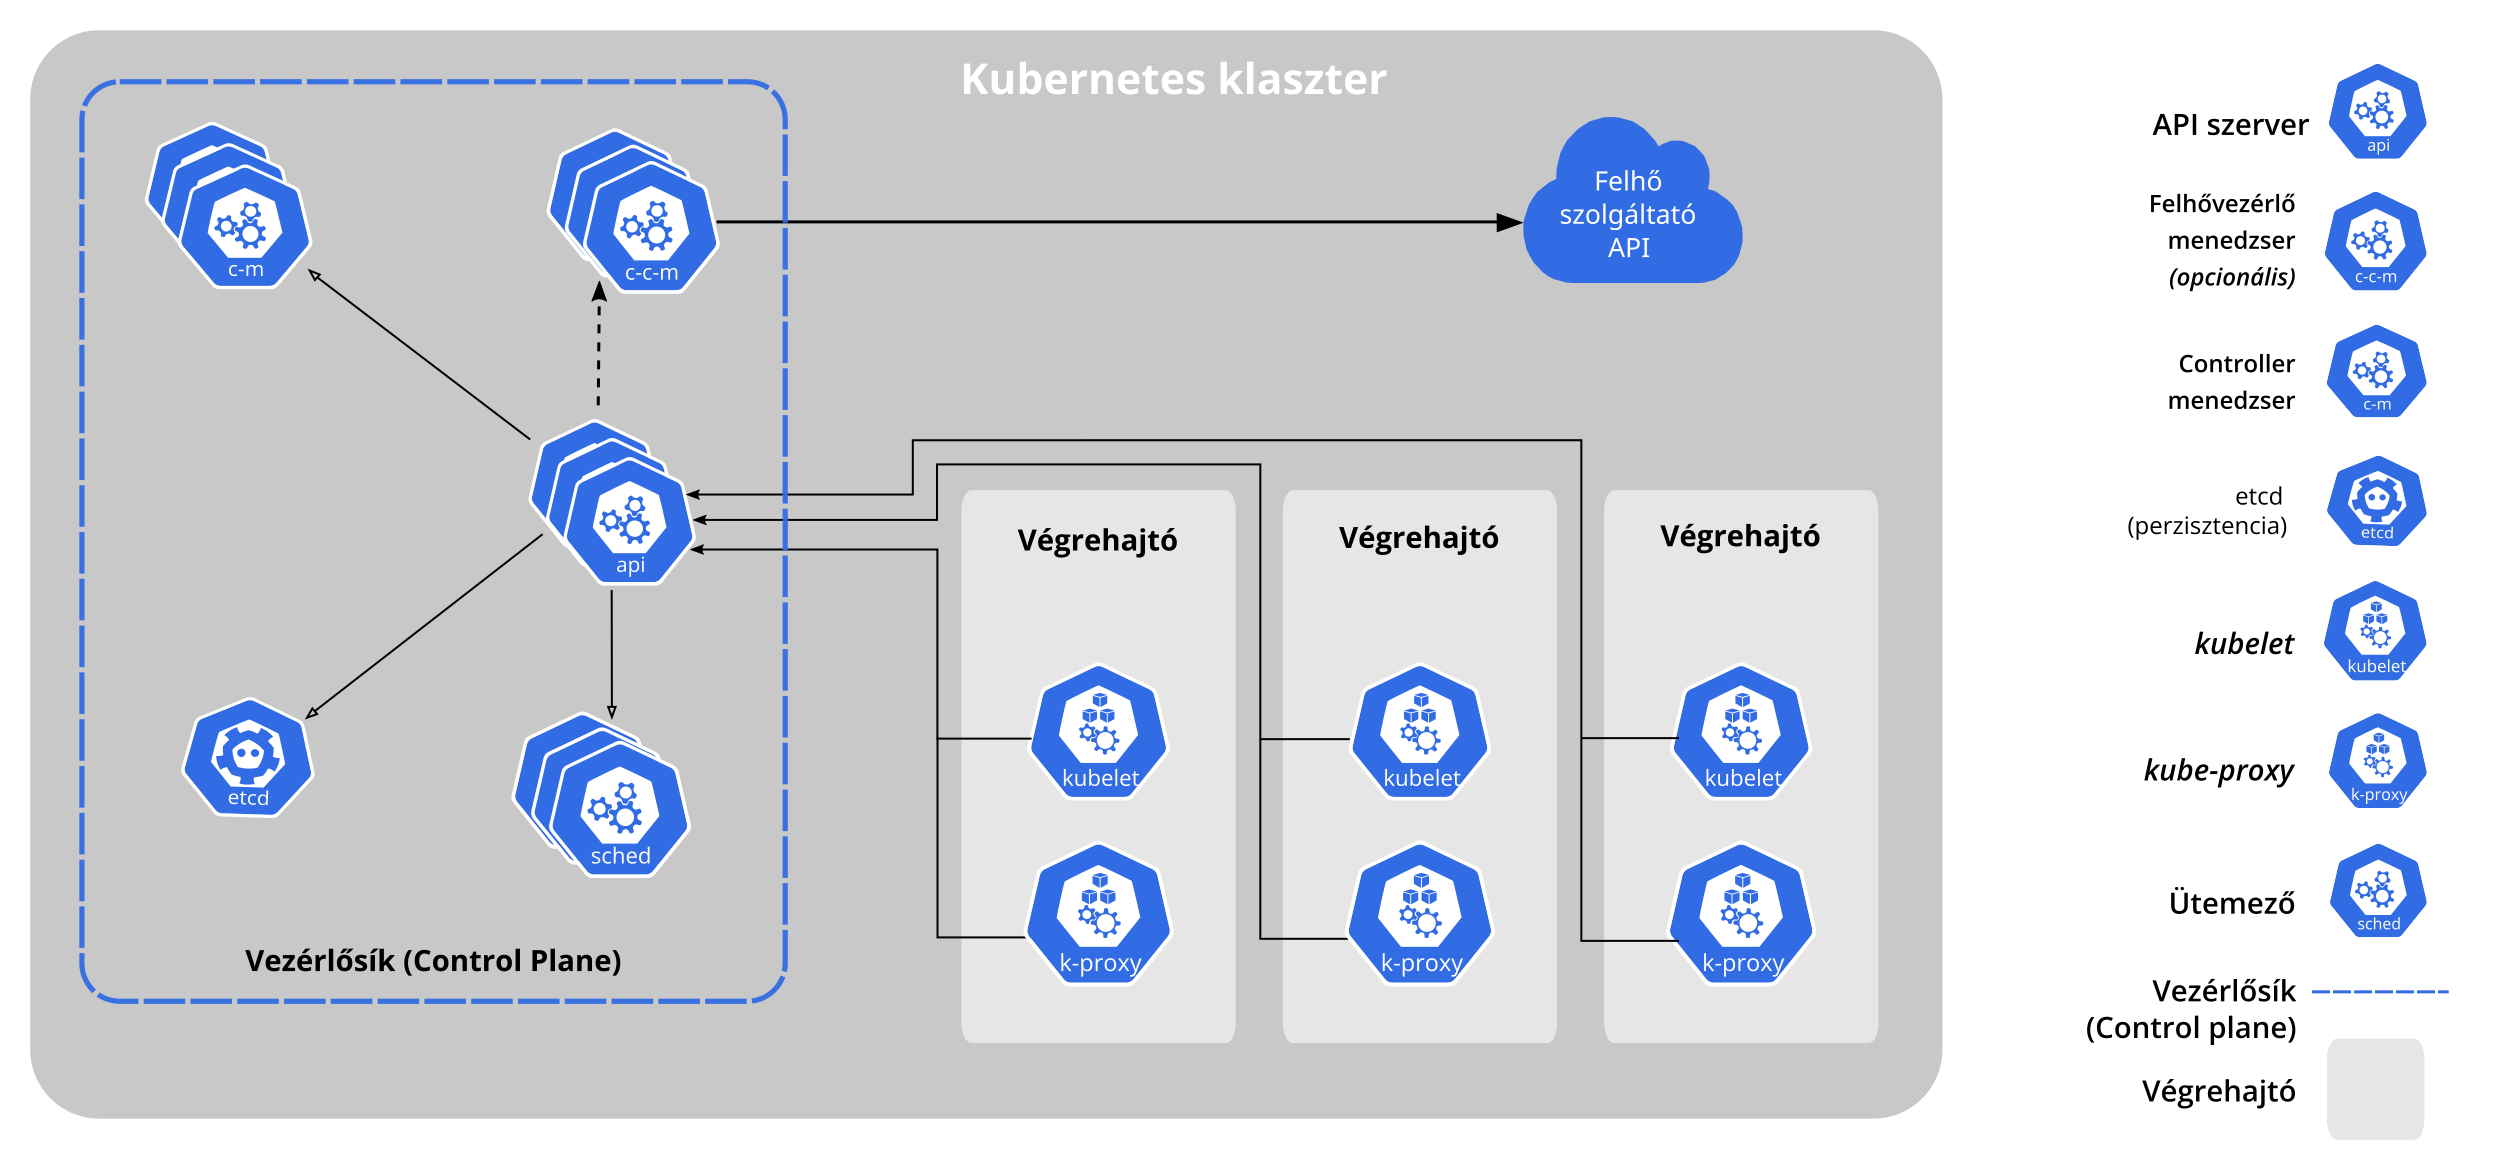
\includegraphics[scale=0.5]{images/survey/kubernetes.png}
        \caption{A Kubernetes architektúrája}
        \label{kubernetes}
\end{figure}

A Kubernetes (\ref{kubernetes}. ábra) egy nyílt forráskódú
konténer-orchestrációs platform, amely automatizálja a konténeres alkalmazások
telepítését, skálázását és kezelését. Eredetileg a Google tervezte, és a Cloud
Native Computing Foundation (CNCF) tartja karban. A Kubernetes egy
többcsomópontos platform, amelyet több fizikai vagy virtuális gépen
(csomóponton) való telepítésre terveztek. Ezáltal biztosítja a magas
rendelkezésre állást és a skálázhatóságot. Lehetővé teszi a fejlesztők számára,
hogy deklaratívan definiálják az alkalmazásaik kívánt állapotát. A Kubernetes
gondoskodik arról, hogy ez az állapot fennmaradjon: kezeli a hibákat, a
terheléselosztást és a skálázást.

A Kubernetes fő komponensei közé tartozik a \textit{master node}
(vezérlőcsomópont) és a \textit{worker node}-ok (munkavégző csomópontok). A
vezérlőcsomópont felelős a klaszter állapotának fenntartásáért, a munkavégző
csomópontok pedig a konténerek tényleges futtatásáért. A Kubernetes deklaratív
konfigurációs fájlokat használ (általában YAML formátumban), amelyekben
leírhatjuk, hogy milyen alkalmazásokat, hány példányban, milyen erőforrásokkal
szeretnénk futtatni.

A Kubernetes legfontosabb absztrakciói:
\begin{enumerate}
        \item \textbf{Pod}: A legkisebb üzemeltethető egység, amely egy vagy több konténert tartalmaz, közös hálózati és tároló erőforrásokkal.
        \item \textbf{Deployment}: Lehetővé teszi a podok deklaratív menedzselését, például a példányszám automatikus skálázását vagy frissítését.
        \item \textbf{Service}: Állandó hálózati elérési pontot biztosít a podokhoz, elrejti a podok dinamikus IP-címét, és lehetővé teszi a terheléselosztást.
        \item \textbf{ConfigMap} és \textbf{Secret}: Konfigurációs adatok és érzékeny információk (például jelszavak) kezelésére szolgálnak.
        \item \textbf{Ingress}: Külső forgalom irányítására szolgáló komponens, amely lehetővé teszi a HTTP(S) forgalom szabályozását, átirányítását a megfelelő szolgáltatásokhoz.
\end{enumerate}

A Kubernetes előnyei közé tartozik a magas rendelkezésre állás, az automatikus
skálázás, az önjavítás (például hibás podok automatikus újraindítása), valamint
a gördülő frissítések támogatása. A platform széles körben támogatott a nagy
felhőszolgáltatók (Google Cloud, AWS, Azure) által, de saját infrastruktúrán is
telepíthető.

A Kubernetes komplexitása miatt kisebb projektek esetén túl komplikált lehet,
azonban nagyvállalati környezetben, microservice-alapú architektúrák esetén
szinte iparági szabvánnyá vált. A Zebrafish fejlesztése során a Kubernetes
által kínált funkcionalitás inspirációként szolgált, azonban a cél egy
egyszerűbb, könnyebben kezelhető, fejlesztőbarát platform létrehozása volt,
amely a Compose-alapú munkafolyamatokat helyezi előtérbe, az egyszerűbb
telepítésekhez, amelyek csak egyetlen kiszolgálót igényelnek.

\section{Használt szoftverek, könyvtárak}

Ebben a fejezetben megvizsgáljuk a fejlesztés során használt szoftvereket a Zebrafish platform fejlesztéséhez.
A Zebrafish platform valóban óriások vállára épül, számos olyan szoftvert használ, amelyek közül néhányat korábban csak szabadalmaztatott platformokba integráltak, mint például a Dockerbe.

Ennek a fejezetnek a célja, hogy áttekintést adjon a felhasznált szoftverekről, valamint rövid magyarázatot arról, hogy miért ezeket a szoftvereket választottuk, és hogy hogyaan járulnak hozzá a Zebrafish működéséhez.

\subsection{A Linux kernel}

A Linux kernel számos alapvető funkciót biztosít a Zebrafish által biztosított konténerizációhoz. A Linux felelős a folyamatok elkülönítésének és erőforrásainak kezeléséért. Elsősorban a Linux névterek (namespaces) funkcióját használjuk a szükséges elszigetelés biztosítására. Másodsorban a rendszer erőforrásainak priorizálására a cgroups (control groups) funkciót használjuk.

A névterek a folyamatok elszigetelését biztosítják azáltal, hogy egy virtuális környezetet hoznak létre a folyamatok egy csoportja számára. Minden névtér úgy tűnik a benne lévő folyamatok számára, hogy egy globális rendszererőforrás saját, elszigetelt példányával rendelkeznek. A Linux kernel többféle névteret biztosít, amelyek közül a legfontosabbak, amelyeket a Zebrafish platformon használunk, a következők:
\begin{itemize}
    \item \textbf{PID névtér:} Elkülöníti a folyamatazonosítókat, ami azt jelenti, hogy a konténeren belüli folyamatoknak saját PID-készletük van. Mivel a PID 1-es folyamat az init folyamat, ő felelős a zombi folyamatok leállításáért és az árva folyamatok kezeléséért. Annak biztosítására, hogy az init folyamat ténylegesen kezelje ezeket a feladatokat, egy speciális init folyamatot (tini) használunk, amely PID 1-ként fut a konténeren belül és megvalósítja ezeket a funkciókat.
    \item \textbf{Hálózati névtér:} Elkülöníti a hálózati interfészeket, útválasztási táblákat és portokat. Minden konténer saját virtuális hálózati veremmel rendelkezik. Ezt használjuk annak biztosítására, hogy a konténerek kommunikálni tudjanak egymással és a gazdarendszerrel anélkül, hogy más konténereket zavarnának. Természetesen ehhez tartozik egy userland réteg is.
    \item \textbf{Mount névtér:} Elkülöníti a fájlrendszert. A különböző mount névterekben lévő folyamatok különböző nézetekkel rendelkeznek a fájlrendszerre. Tiszta és elszigetelt fájlrendszert biztosítunk minden konténer számára. Egy konténerben végrehajtott változtatások nem befolyásolhatják a többit.
    \item \textbf{User névtér:} Elkülöníti a felhasználói- és csoportazonosítókat, lehetővé téve, hogy egy folyamatnak egy konténeren belül egy normális, nem root jogosultságú felhasználója legyen. Ez nagyon fontos a biztonság szempontjából, mivel a konténereket ezáltal csökkentett jogosultságokkal tudjuk futatni.
\end{itemize}

A cgroups segítségével kiosztjuk a rendszer erőforrásait. Például a CPU-nak, a memóriának és az I/O-nak a prioritását és határértékeit (limitjeit) tudjuk meghatározni egy folyamatgyűjtemény számára. Ezáltal egyetlen egy konténer nem tudja monopolizálni a rendszer erőforrásait. Ha monopolizálni tudná, akkor negatív hatással lehetne a többiekre. Míg az ütemező alapból elég jó munkát végez az erőforrások elosztásában, a cgroups segítségével korlátokat és kéréseket tehetünk.

A Zebrafish platform számára alapként szolgál a Linux kernel. Rendelkezik mindazon fájlrendszer-kezeléshez és biztonsághoz szükséges kényelmi funkciókkal, amik biztosítják, hogy nem kell újra feltalálnunk a spanyol viaszt: számos fájlrendszert támogat, amelyek közül néhány erős adatkonzisztencia-garanciát biztosít; támogatja az olyan fejlett funkciókat, mint például az SMB, az NFS és az NBD, amelyek elengedhetetlenek a Zebrafish távoli fájlrendszer-képességeihez; és olyan biztonsági modellt biztosít, amely lehetővé teszi, hogy a konténereket csökkentett jogosultságokkal futtassuk, biztosítva, hogy még ha egy konténer veszélybe is kerül, a kár korlátozott legyen.

\subsection{Buildroot}

A Buildroot egy egyszerű, hatékony és könnyen használható eszköz egyedi beágyazott Linux rendszerek létrehozására keresztkompilálással (\textit{cross-compilation}). Automatizálja a teljes Linux-rendszer építésének folyamatát, beleértve a keresztkompilációs eszköztárat, a gyökérfájlrendszert, a kernelképet (\textit{kernel image}) és a bootloadert (\textit{EFI stub} vagy \texttt{syslinux}). Mivel a cél egy minimális, hatékony operációs rendszer létrehozása volt, amely \texttt{ARM64} és \texttt{x86\_64} architektúrákon egyaránt futtatható, a Buildroot-ra esett a választás.

A Zebrafish tervezése során több build rendszert is kipróbáltunk, köztük a Yocto Projectet, azonban a Buildrootra esett a választásunk az egyszerű konfigurálhatósága és a gyors ütemű közösségi fejlesztése miatt. A gyakori frissítések biztosítják, hogy mindig a legújabb szoftverekre építhetjük a Zebrafish platformot. A Kconfig-alapú konfigurációs rendszerének egyszerűsége pedig kivételesen egyszerűvé teszi az operációs rendszer képének beállítását.

A Buildroot azt is lehetővé teszi, hogy a generált lemezképekhez létrehozzunk egy \textit{software bill of materials}-t (SBOM), ami elengedhetetlen ahhoz, hogy tisztában legyünk azzal, hogy valójában milyen szoftvereket futtatunk a szervereinken. A SBOM segítségével nyomon követhetjük az összes beépített szoftverkomponenst és azok verzióit.

A projekt fejlesztése során lehetőség nyílt arra, hogy a Buildroot közösségnek változtatásokat visszaadjunk. Ez magába foglalta a javítások küldését a hivatalos levelezési listára. Értékes tapasztalat volt számomra, hiszen a Buildroot közösség, a Linux közösséghez hasonlóan, még mindig levelezőlistákon keresztül kommunikál.

A jövőre nézve a \texttt{bootc} projekt a bootolható konténer alapú operációs rendszerek érett eszközévé válhat. A \texttt{bootc} használatának további vizsgálata indokolt. Jelentős előnyöket kínálhat a rendszerfrissítések és a rendszerkezelés terén.

\subsection{Containerd és Nerdctl}

A Zebrafish platformon a konténerek futtatására a \textit{containerd} szolgáltatást használjuk. A \textit{containerd} biztosítja a konténerek életciklusának kezelését, beleértve a konténerek indítását, leállítását és monitorozását. Azonban nem biztosít lehetőséget összetettebb műveletekre, mint például Compose projektek kezelésére vagy a hálózati paraméterek beállítására.

A nerdctl egy parancssori eszköz, amely Docker-kompatibilis CLI-t biztosít a containerd számára. A nerdctl lehetővé teszi konténerek, képek és hálózatok kezelését, valamint támogatja a Compose projekteket is. A leggyakrabban használt parancsok közé tartoznak:

\begin{itemize}
        \item \texttt{nerdctl run}: Új konténer indítása egy adott imageből.
        \item \texttt{nerdctl ps}: Futtatott konténerek listázása.
        \item \texttt{nerdctl images}: Elérhető konténer image-ek listázása.
        \item \texttt{nerdctl build}: Saját image építése Dockerfile alapján.
        \item \texttt{nerdctl compose up}: Compose projekt indítása.
        \item \texttt{nerdctl compose down}: Compose projekt leállítása.
        \item \texttt{nerdctl logs}: Konténer naplóinak megtekintése.
\end{itemize}

A nerdctl CLI két legnagyobb problémája a multi-Compose projektek támogatásának hiánya, valamint az általa használt rossz zárási mechanizmus.  Még az egy-Compose-os projekteken belül is az image-ek lehúzása registryből csupán egymás után lehetséges, ami hosszú időt vehet igénybe, ha az image-ek nagyok. Ha egy image-t több helyen is használunk, akkor külön-külön lehúzza  ugyanazt. Esély sincs arra, hogy egy másodperc töredékén belül változás történt volna a feltöltött imageben.

A zárolási mechanizmus is problémás, mivel a teljes Compose környezetet zárolja, megakadályozva, hogy több Compose parancs párhuzamosan fusson. Ez a mi esetünkben jelentős korlátozást jelent, mivel gyakran kell egyszerre több Compose projektet futtatnunk.

A hálózat beállításához a nerdctl CNI integrációját használjuk, míg a Compose projektek kezelésére saját megoldást javaslunk, amely a containerd API-t használja. Ez a megoldás kompatibilis lesz a meglévő nerdctl CLI-al, így a Zebrafish CLI-al indított konténerek a nerdctl CLI-al is kezelhetők lesznek.

\subsection{CNI}

A CNI (Container Network Interface) egy szabványos interfész a konténeres hálózatok kezelésére. A Zebrafish a CNI-t használjuk a konténerek közötti hálózati kommunikáció biztosítására. A CNI különböző hálózati plugineket ad számunkra, amelyekkel beállíthatjuk a konténerek hálózati konfigurációját.

A CNI pluginok Go nyelven íródtak, és a következő pluginokat használjuk a Zebrafish-ben:
\begin{itemize}
        \item \texttt{bridge}: A legegyszerűbb hálózati plugin, amely egy Linux bridge-t hoz létre a konténerek számára. Lehetővé teszi, hogy a konténerek kommunikáljanak egymással és a gazdarendszerrel.
        \item \texttt{host-local}: Biztosítja a konténerek számára az IP-címeket. Segítségével dinamikusan osztunk ki IP-címeket a konténereknek.
        \item \texttt{firewall}: Tűzfal-szabályok alkalmazását implementálja.
        \item \texttt{portmap}: Segítségével a konténerek portjait a gazdagép portjaira le lehet leképezni (\textit{port forwarding}), így a kívülről érkező forgalom elérheti a konténereket.
        \item \texttt{tuning}: Lehetővé teszi a hálózati interfészek MTU paraméterének beállítását.
\end{itemize}

\subsection{Rust}

A Zebrafish egyes moduljainak fejlesztéséhez a Rust programozási nyelvet választottuk. A Rust egy modern, rendszerszintű programozási nyelv, amely a biztonságra és a teljesítményre összpontosít. A Rust egyik legnagyobb előnye a memóriabiztonság, amelyet a nyelv beépített tulajdonságai garantálnak, így elkerülhetők a gyakori hibák.

A Rust nyelv segítségével a fejlesztők biztosítani tudják az időbeli biztonságot és a memóriabiztonságot. A Rust fordító a fordítási időben széleskörű ellenőrzéseket végez, ami segít a lehetséges hibák korai felismerésében a fejlesztési folyamat során. Egyre nehezebb olyan kódot írni, amely nem kezeli az összes lehetséges esetet. Természetesen továbbra is lehetséges hibás kódot írni, de a fordító a hibák nagy részét már a kód futtatása előtt elkapja.

A Rust programozási nyelvben a két legfontosabb absztrakciós eszköz a \texttt{struct} és a \texttt{trait}. A \texttt{struct} típusok lehetővé teszik saját, összetett adattípusok definiálását, amelyek mezőket (fieldeket) tartalmaznak, hasonlóan más nyelvek osztályaihoz. Az \texttt{impl} blokk segítségével metódusokat rendelhetünk ezekhez a struktúrákhoz, így viselkedést adhatunk az adatokhoz.

A \texttt{trait} egyfajta interfész (szerződés), amely meghatározza, hogy egy típusnak milyen metódusokat kell implementálnia. Egy \texttt{struct} egy vagy több \texttt{trait}-et is implementálhat, így biztos megfelel annak a szerződésnek.

\subsection{Tokio}

A Zebrafishen belül a Tokio aszinkron futtatókörnyezetet használjuk a Rust nyelvben írt komponensek számára. A Tokio egy aszinkron I/O könyvtár, amely lehetővé teszi nagy teljesítményű, párhuzamosan futó alkalmazások fejlesztését. A Tokio segítségével könnyedén kezelhetjük az aszinkron műveleteket, főleg a hálózati kommunikációkat.

Más aszinkron futásidejű programokhoz képest a Tokio egy nagyon jól átgondolt és tervezett könyvtár. Gazdag funkciókészletet biztosít, beleértve az időzítőket, a csatornákat és a feladatütemezést, ami alkalmassá teszi komplex alkalmazások építésére. Úgy tapasztaltam, hogy a más nyelveken található aszinkron futásidejű futásidő, például a Python asyncio, nem olyan jól megtervezett és átgondolt, mint a Tokio.

A Tokiónak köszönhetően a Zebrafish képes több image letöltésére egyidejűleg, így a rendszer frissítése és karbantartása gyorsabbá válik, az új szolgáltatások bevezetése pedig gördülékenyebb.
        %----------------------------------------------------------------------------
\chapter{A rendszer specifikációja} \label{chapter2}
%----------------------------------------------------------------------------

\section{Felhasználói követelmények}

A felhasználói követelmények részletezik a felhasználói elvárásokat a Zebrafish rendszerrel szemben. Ez a fejezet határozza meg azokat a követelményeket, amelyeknek a rendszernek meg kell felelnie a célközönség igényeinek kielégítése érdekében.

A Zebrafish platform négy fő felhasználói csoportra összpontosít, mindegyiknek különböző igényeivel és munkafolyamataival:

\begin{enumerate}
  \item \textbf{Rendszergazdák} - akik az összes összetett, több Compose-projektből álló egységeket kezelhetik
  \item \textbf{Projektmenedzserek} - akik a Zebrafish platformon saját alkalmazásokat kezelnek
  \item \textbf{Fejlesztők} - akik több Compose-projektből álló alkalmazásokat fejlesztenek
  \item \textbf{Szervízfelhasználók} - akik automatizált módon hozzáférhetnek a Zebrafish platformhoz CI/CD rendszerekből
\end{enumerate}

\subsection{Rendszergazdák}

A rendszergazdák felelősek a Zebrafish operációs rendszer telepítéséért, karbantartásáért és felügyeletéért. Elvárásaik a stabilitásra, hatékonyságra és egyszerű kezelhetőségre összpontosítanak.

\begin{requirementstable}
  \caption{Felhasználói követelmények rendszergazdák számára} \\
  
  \requirementtitlewordwrap{Rendszertelepítés,\\image-kezelés} &
  \requirementslist{
    \item A rendszergazdáknak képesnek kell lenniük az egész rendszer összes konténer image-ének egyetlen paranccsal történő letöltésére, frissítésére
    \item A Compose-projektek első telepítése során az image-ek letöltésének gyorsnak kell lennie, kihasználva a párhuzamos letöltési lehetőséget
    \item A rendszer nem pazarolhatja a lemezterületet; a megosztott image-rétegeket csak egyszer szabad tárolni
    \item Az image-ek automatikus frissítésének támogatottnak kell lennie a teljes rendszerre vonatkozóan
  } \\

  \requirementtitlewordwrap{Rendszerfrissítés és karbantartás} &
  \requirementslist{
    \item A teljes rendszer frissítésének gyorsnak és atomi műveletnek kell lennie
    \item A frissítési folyamatnak egyszerűnek és könnyen kezelhetőnek kell lennie
    \item A rendszernek stabilnak kell maradnia egy frissítést követően
    \item Frissítés során nem szabad elvesztődnie a konfigurációs fájloknak
    \item Frissíŧés után a rendszer különleges beavatkozás nélkül kell működjön
  } \\

  \requirementtitlewordwrap{Rendszerfelügyelet és monitorozás} &
  \requirementslist{
    \item A rendszergazdáknak egyetlen paranccsal átfogó képet kell kapniuk a rendszer állapotáról
    \item Az állapotellenőrzésnek tartalmaznia kell, hogy mely konténerek futnak és melyek állnak
    \item A platformnak terminál alapú felhasználói felületet (TUI) kell biztosítania a rendszer vizuális áttekintéséhez
  } \\

  \requirementtitlewordwrap{Projekt- és konténerkezelés} &
  \requirementslist{
    \item A rendszergazdáknak képesnek kell lenniük egy teljes Compose-projekt leállítására egyetlen paranccsal
    \item Lehetőséget kell biztosítani az összes futó konténer azonnali újraindítására
    \item A független projektek nem indulhatnak újra feleslegesen, amikor egy másik, nem kapcsolódó projekt függőségei frissülnek
    \item A projektek közötti függőségeket a rendszernek automatikusan fel kell ismernie és kezelnie
    \item A rendszergazdáknak képesnek kell lenniük az alkalmazások naplóinak megtekintésére és kezelésére
    \item A rendszergazdák az összes projektet láthatják és módosíthatják a fájlrendszerből
  } \\

  \requirementtitlewordwrap{Hálózatkezelés} &
  \requirementslist{
    \item A hálózatokat a rendszernek proaktívan kell létrehoznia
    \item A hálózatok konfigurációját meg kell tudja adni a Compose-fájlokban
    \item A rendszergazdának nem kell manuálisan beavatkoznia a hálózatok létrehozásába
  } \\

  \requirementtitlewordwrap{Adatbiztonság és helyreállítás} &
  \requirementslist{
    \item A szerver adatainak automatikusan szinkronizálására lehetőséget kell adni
    \item Az adatok integritását biztosítani kell
    \item Katasztrófa esetén gyors helyreállítási mechanizmusnak kell rendelkezésre állnia
  }
\end{requirementstable}

\subsection{Projektmenedzserek}

A projektmenedzserek a Zebrafish platformot saját alkalmazásaik kezelésére használják. Fő feladatuk a projektek létrehozása, konfigurálása és karbantartása. Fontos megemlíteni, hogy a projektmenedzserek nem látnak rá más felhasználók Compose-projektjeire, a rendszernek biztosítania kell a projektek közti izolációt.

\begin{requirementstable}
  \caption{Felhasználói követelmények projektmenedzserek számára} \\

  \requirementtitlewordwrap{Projektek karbantartása} &
  \requirementslist{
    \item Szükséges, hogy saját projektjeiket láthatni tudják a fájlrendszerből
    \item Képesnek kell lenniük új Compose-projektek létrehozására a fájlrendszerből
    \item Terminálhozzáférést kell biztosítani a projektmenedzserek számára, hogy kezelhessék projektjeiket
    \item Elvárják, hogy a projektek egymással tudjanak kommunikálni a megosztott hálózatokon keresztül
    \item A projektmenedzsereknek nem láthatják más felhasználók projektjeit, csak a sajátjukat
  } \\

  \requirementtitlewordwrap{Erőforrásokhoz való hozzáférés} &
  \requirementslist{
    \item A projektmenedzserek saját projektjeiket hozzá kell tudják más projektmenedzserek hálózataihoz kapcsolni
    \item A hálózati névfeloldásnak működnie kell a projekt határain belül
    \item A projektmenedzsereknek képesnek kell lenniük a saját hálózataik konfigurálására
    \item A volumok egymás között nem szabad megoszthatóak legyenek, csak a saját projektjeikhez férhetnek hozzá
  }
\end{requirementstable}

\subsection{Fejlesztők}

A fejlesztők a Zebrafish platformot alkalmazásaik fejlesztésére, tesztelésére és futtatására használják. Számukra a legfontosabb a megszokott munkafolyamatok támogatása és a konténerek közötti zökkenőmentes kommunikáció.

\begin{requirementstable}
  \caption{Felhasználói követelmények fejlesztők számára} \\

  \requirementtitlewordwrap{Compose-kompatibilitás} &
  \requirementslist{
    \item A Compose-projektek felépítésének és konfigurációjának menete nem szabad eltérjen a megszokott Compose munkafolyamatoktól
    \item A fejlesztőknek nem kell új szintaxist vagy struktúrát tanulniuk a meglévő Compose fájljaik használatához
    \item Az összes standard Compose direktívának támogatottnak kell lennie (pl. services, networks, volumes)
  } \\

  \requirementtitlewordwrap{Multi-Compose projekt támogatás} &
  \requirementslist{
    \item A különböző Compose-projektekben futó konténereknek képesnek kell lenniük egymással kommunikálni
    \item A projektek közötti hálózati kommunikáció felépítésének zökkenőmentesnek kell lennie
    \item A szolgáltatások közötti névfeloldásnak működnie kell projekt határokon keresztül is
    \item A megosztott erőforrások (volumes, networks) nem kell projekteken keresztül használhatóak legyenek
  } \\

  \requirementtitlewordwrap{CLI integráció} &
  \requirementslist{
    \item A Zebrafish CLI-val készített konténerek kezelhetőek kell legyenek a containerd és nerdctl parancsokkal
    \item A CLI parancsok megszokott Docker Compose parancsokhoz hasonlóan működjenek
    }
\end{requirementstable}

\subsection{Szervízfelhasználók}

A szervízfelhasználók automatizált rendszerekből, például CI/CD pipeline-okból férnek hozzá a Zebrafish rendszerhez. Számukra a legfontosabb, hogy a rendszer könnyen automatizálható legyen.

\begin{requirementstable}
  \caption{Felhasználói követelmények szervízfelhasználók számára} \\

  \requirementtitlewordwrap{Automatizált hozzáférés} &
  \requirementslist{
    \item A szervízfelhasználóknak képesnek kell lenniük a Zebrafish rendszerhez parancssori eszközökön keresztül hozzáférni
    \item A rendszerre csatlakozni kell lehessen a CI/CD rendszerekből, például GitHub Actions-on keresztül
    \item Az automatikus hozzáférés képes kell legyen terminál alapú parancsokat futtatni
    \item A különböző compose parancsok nem szabad manuális beavatkozást igényeljenek
  } \\

  \requirementtitlewordwrap{Biztonságos hozzáférés} &
  \requirementslist{
    \item A hozzáférés biztonságos kell legyen: nem szabad illetéktelen felhasználók számára elérhetővé tenni
    \item A szervízfelhasználók csak a saját projektjeikhez férnek hozzá
  }
\end{requirementstable}

\section{Rendszerkövetelmények}

\subsection{Funkcionális követelmények}

Az alkalmazásnak olyan felülettel kell rendelkeznie, amely lehetővé teszi a felhasználók számára a projektek, konténerek és image-ek kezelését. A Zebrafish választott felülete egy parancssori felület (CLI - command line interface), amely parancsok sorát biztosítja a Docker Compose projektek, image-ek és konténerek kezeléséhez. A CLI-nak lehetővé kell tennie a felhasználók számára olyan általános feladatok elvégzését, mint a projektek indítása, leállítása és naplóinak megtekintése.

\begin{requirementstable}
  \caption{Funkcionális követelmények - Rendszerkezelés} \\

  \requirementtitlewordwrap{Rendszer-\\kompatibilitás} &
  \requirementslist{
    \item A Zebrafish rendszer kompatibilis kell legyen a \texttt{x86\_64} és \texttt{ARM64} architektúrákkal
    \item A Zebrafish kell támogassa a BIOS és UEFI indítást is
    \item A rendszer futtatható kell legyen a legelterjedtebb virtualizációs platformokon (KVM és VMware)
  }

  \requirementtitlewordwrap{Parancssori interfész (CLI)} &
  \requirementslist{
    \item A CLI-nek SSH-interfészen keresztül kell elérhetőnek lennie.
    \item Letölthető kell legyen az összes definiált Compose-projekt összes image párhuzamosan egy CLI parancs lefuttatásával 
    \item Megjeleníthető kell a rendszer általános állapota, beleértve a futó és leállított konténereket
    \item Frissíthető kell legyen a rendszer magja egyetlen parancs segítségével
    \item A rendszer különböző komponensei (pl. Crony, containerd) menedzselhetőek kell legyenek a CLI-on keresztül
    \item Az SSH-interfésznek támogatnia kell a Zebrafish operációs rendszerben elérhető összes többi parancsot is.
  } \\
 
  \requirementtitlewordwrap{Compose projektkezelés} &
  \requirementslist{
    \item A Compose-fájloknak kompatibilisnek kell lenniük a Compose V2 formátumával
    \item A hagyományos Compose-projektekhez hasonlóan a multi-Compose projekteket is konténerek létrehozásával és karbantartásával kell megvalósítani
    \item A Zebrafish által létrehozott konténereket a szabványos containerd és nerdctl parancsokkal is lehet kezelni.
    \item A parancsoknak támogatniuk kell a \texttt{-f} flag-et alternatív compose fájlok megadásához
  } \\

  \requirementtitlewordwrap{Image és tárolókezelés} &
  \requirementslist{
    \item Az image-kezelésnek kompatibilisnek kell lennie az OCI formátummal
    \item A rendszernek képesnek kell lennie a containerd image-ek kezelésére
    \item A rendszernek támogatnia kell a párhuzamos image letöltést a Tokio aszinkron futtatókörnyezet használatával
  }
\end{requirementstable}

\begin{requirementstable}
  \caption{Funkcionális követelmények - Hálózat és biztonság} \\

  \requirementtitlewordwrap{Hálózatkezelés} &
  \requirementslist{
    \item A rendszernek automatikusan létre kell hoznia a Compose-fájlokban definiált hálózatokat
    \item A CNI pluginokat (bridge, host-local, firewall, portmap, tuning) támogatni kell
    \item A multi-project hálózati kommunikációt külön hálózati névterekkel kell kezelni
    \item A szolgáltatások közötti névfeloldást DNS-sel kell biztosítani
  } \\

  \requirementtitlewordwrap{Biztonság} &
  \requirementslist{
    \item A rendszer magjának megváltoztathatatlannak kell lennie (immutable)
    \item SSH hozzáférés csak nyilvános kulcsos hitelesítéssel engedélyezett
    \item Port knocking mechanizmust kell implementálni az SSH védelmére
    \item DNS over HTTPS (DoH) kötelező az összes DNS lekérdezéshez
    \item HTTP/3 alapértelmezett protokoll a külső kommunikációhoz
  } \\

  \requirementtitlewordwrap{Adatkezelés} &
  \requirementslist{
    \item A ZFS fájlrendszernek biztosítania kell az adatintegritást
    \item Automatikus pillanatfelvételek készítése konfigurálandó időközönként
    \item Inkrementális replikáció támogatása távoli szerverekre
    \item A konfigurációs változtatások overlay fájlrendszeren keresztüli kezelése
  }
\end{requirementstable}

\subsection{Nem funkcionális követelmények}

Külső követelményekkel olyan feltételeket határozunk meg, amelyeknek a Zebrafish rendszernek meg kell felelnie, hogy illeszkedjen a szélesebb technológiai, jogi és társadalmi környezetbe.

\begin{requirementstable}
  \caption{Külső követelmények (external requirements)} \\

  \requirementtitlewordwrap{Szabványok és kompatibilitás} &
  \requirementslist{
    \item A rendszernek teljes mértékben kompatibilisnek kell lennie az OCI (Open Container Initiative) szabványaival
    \item A Compose fájloknak követniük kell a Docker Compose V2 specifikációt
    \item A container image formátumoknak támogatniuk kell az iparági szabványokat (Docker, OCI)
  } \\

  \requirementtitlewordwrap{Jogi megfelelőség} &
  \requirementslist{
    \item Minden szállított szoftverkomponens licensze kompatibilis kell legyen a rendszer nyílt forráskódú licenszével
    \item A rendszernek követnie kell az országok közti szoftverátadási törvényeket
  } \\

  \requirementtitlewordwrap{Interoperabilitás} &
  \requirementslist{
    \item A rendszernek képesnek kell lennie szabványos CI/CD rendszerekkel való integrációra
    \item Támogatnia kell a szabványos monitorozó rendszerekkel való integrációt (Prometheus, Grafana)
    \item Támogatnia kell a konténerfuttató platformokkal való együttműködést (containerd)
  }
\end{requirementstable}

\begin{requirementstable}
  \caption{Termékkövetelmények (product requirements)} \\

  \requirementtitlewordwrap{Hatékonyság} &
  \requirementslist{
    \item A lemezhasználat nem haladhatja meg a 256 MB-ot az alaprendszer esetében
    \item Az alap memóriahasználat nem haladhatja meg a 512MB-ot alapkonfigurációban
    \item A lokális hálózati névfeloldásnak 0.2 ms-nál rövidebb válaszidővel kell működnie
    \item A hálózati teljesítmény nem degradálódhat jelentősen a projektek számának növekedésével
  } \\

  \requirementtitlewordwrap{Gyorsaság} &
  \requirementslist{
    \item Az image-ek letöltése a lehető leggyorsabb kell legyen, kihasználva teljesen a hálózatot
    \item Megfelelően gyors hálózati kapcsolat esetén (1 Gbit) a rendszernek képesnek kell lennie 20 konténerkép frissítésére kevesebb mint egy perc alatt.
  } \\

  \requirementtitlewordwrap{Megbízhatóság} &
  \requirementslist{
    \item A rendszernek támogatnia kell legalább 30 egyidejűleg futó konténert
    \item A rendszernek képesnek kell lennie a konténerek automatikus újraindítására hiba esetén
    \item A rendszertől le kell lehessen kérni a futó konténerek állapotát és naplóit
    \item A frissítések után a rendszernek konzisztens és stabil állapotban kell maradnia
  }
\end{requirementstable}

\begin{requirementstable}
  \caption{Szervezési követelmények (organizational requirements)} \\

  \requirementtitlewordwrap{Integrációs követelmények} & 
  \requirementslist{
    \item A Zebrafish automatikusan integrálódik a meglévő ZFS storage rendszerekkel
    \item A Zebrafish-nek a meglévő eszközökkel, a Prometheusszal és a Grafanával nyomon követhetőnek kell maradnia
    \item A Zebrafish-nek képesnek kell lennie a meglévő CI/CD rendszerekkel való együttműködésre, mint például GitHub Actions
    \item A rendszer integrálható kell legyen SSH kapcsolatok révén (parancsok futtatásávl)
  } \\

  \requirementtitlewordwrap{Fejlesztési követelmények} &
  \requirementslist{
    \item A forráskód nyilvánosan elérhető GitHub repository-ban
    \item Folyamatos integráció (CI) minden commit után
    \item Dokumentáció szükséges a rendszer telepíŧéséről
  }
\end{requirementstable}
        \chapter{Tervezés} \label{chapter3}

\section{A szoftver architektúrája}

\begin{figure}[!h]
	\centering
        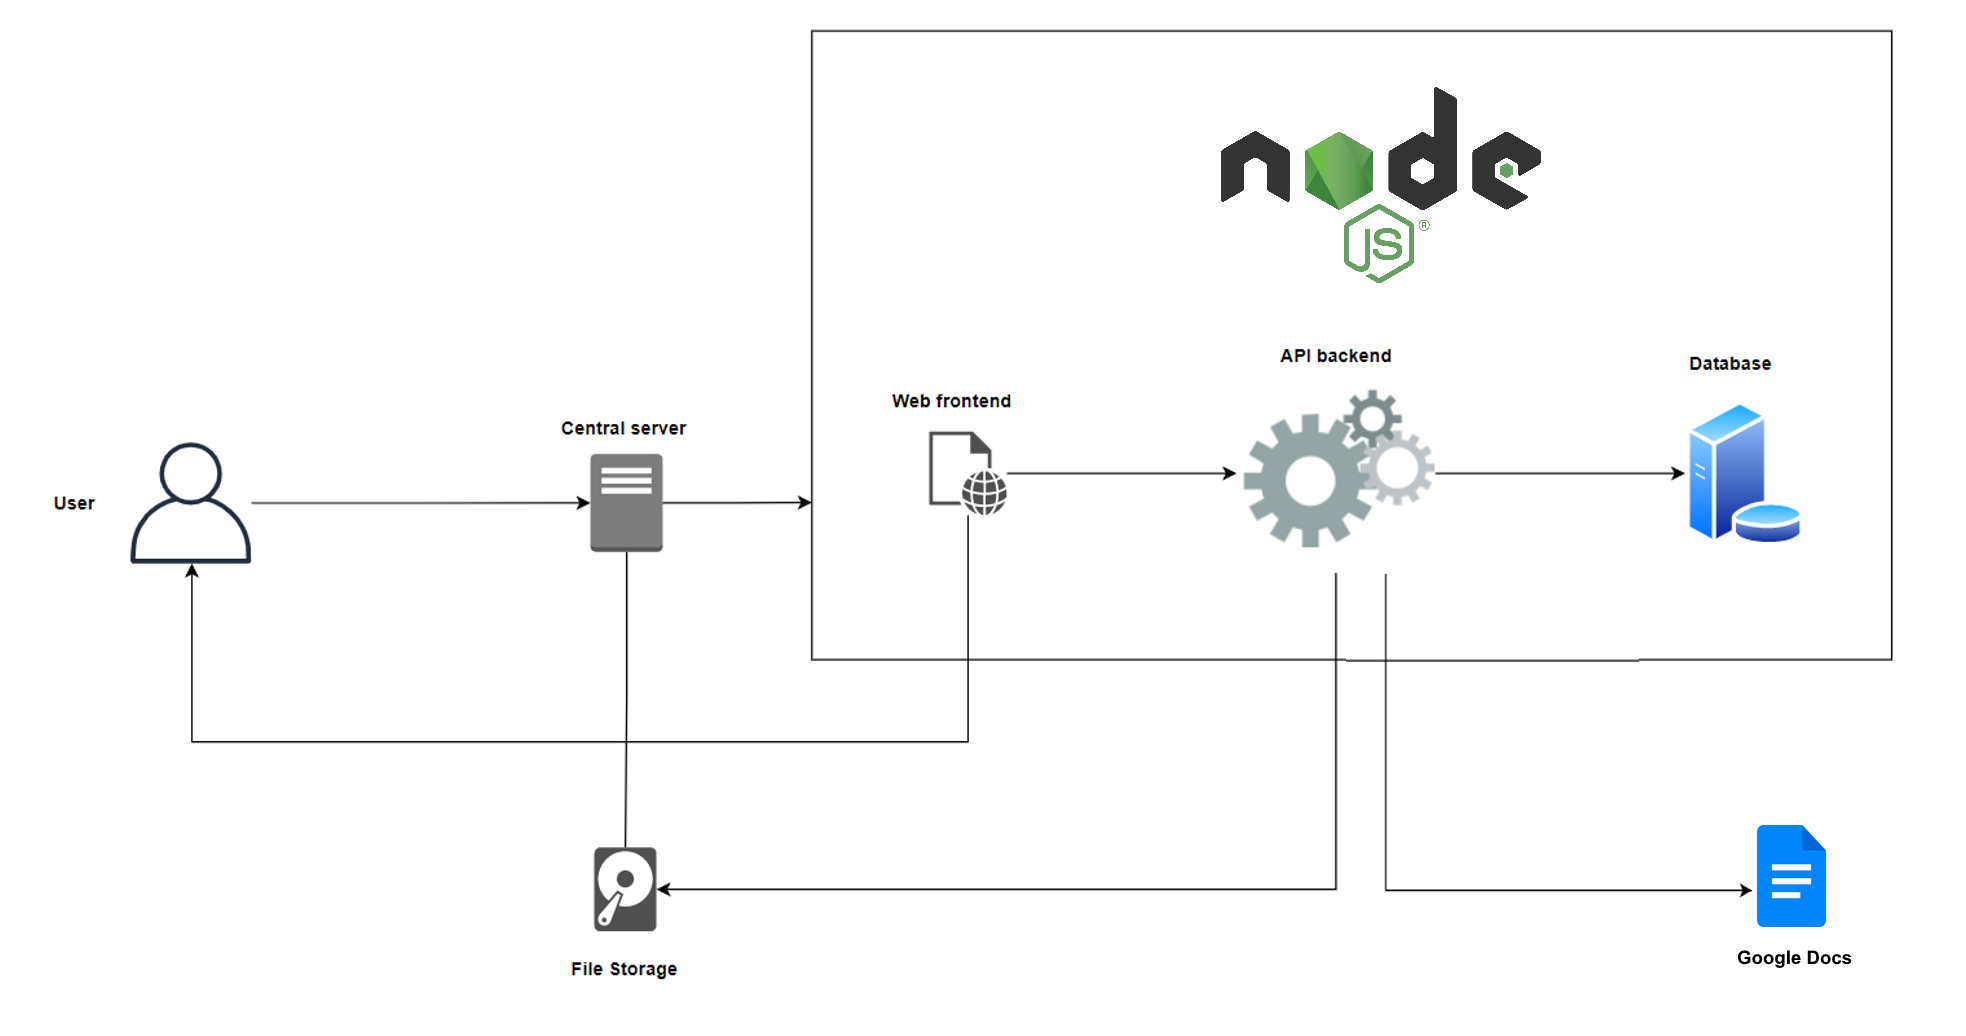
\includegraphics[scale=0.3]{images/software/architecture.png}
	\caption{A Zebrafish OS architektúrája, felülnézetből}
        \label{architecture}
\end{figure}

A Zebrafish operációs rendszer egy valós igényből született. Célunk az, hogy a konténereket egy szervergépen futtassuk egy modern operációs rendszeren, amely nem igényli ok nélkül függőségek sokaságát. Egy olyan biztonságos alapot szerettünk volna létrehozni, amelyet konténeres munkafolyamatok, például alkalmazások és weboldalak futtatására lehet használni.

A legtöbb operációs rendszer, például a Debian és az Ubuntu nem alkalmas erre a célra, mert túlságosan általánosak, és emiatt felesleges függőségeket hordoznak magukkal. Nem elég biztonságosak, és nem úgy tervezték őket, hogy konténeres környezetet futtassanak. Esettanulmány: az operációs rendszer egyetlen frissítése megtörheti az egész rendszer biztonságát. Egy Debian frissítés inspirálta a Zebrafish-t, mivel az egyik éles szerverem tűzfalai egyetlen csomagfrissítés után leálltak. Ez egy éles szerver esetében elfogadhatatlan, biztonsági résekhez vezethet. Ezért hoztuk létre a Zebrafish-t.

A Zebrafish fő ötlete, hogy egy immutable alapot biztosítson, amely képes konténerek futtatására. A Zebrafish egyetlen artifactként kerül kibocsátásra, amely bármely modern \texttt{x86\_64} vagy \texttt{ARM64} gépen elindítható. Az artifact két komponenst tartalmaz:
\begin{itemize}
    \item \textbf{Kernel} - A Linux kernel, amelyet a Zebrafish a rendszerindításhoz használ.
    \item \textbf{Gyökér fájlrendszer} - A Zebrafish gyökér fájlrendszere. Tartalmaz minden szükséges komponenst a Zebrafish OS futtatásához, beleértve a konténer futtattókörnyezetet, a rendszerdémonokat és a CLI eszközöket. Futás közben egy RAM-diskként él, biztosítva, hogy a rendszer mindig a memóriában cachelve legyen.
\end{itemize}

Minden frissítés során egy új artifact kerül kibocsátásra, amely tartalmazza a kernel és a root filesystem új verzióját. A Zebrafish frissítését egy manifest állomány segítségével végezzük, amely tartalmazza a kernel és a root filesystem hash értékét. A manifest állomány segítségével ellenőrizzük, hogy van-e szükség frissíŧésre, illetve hogy a letöltött frissítések helyesek-e. 

A Zebrafish operációs rendszer a következő nagyobb komponensekből áll:

\begin{enumerate}
        \item \textbf{Linux kernel} - A legújabb mainline kiadásra épül. Biztosítja a legújabb funkciók és frissítések elérhetőségét az optimális teljesítmény érdekében.
        \item \textbf{Gyökér fájlrendszer} - Tartalmazza az összes alapvető komponenst, amelyek szükségesek a Zebrafish operációs rendszer működéséhez:
        \begin{itemize}
                \item \textbf{Containerd} - Konténerek futtatására használt, könnyű és hatékony konténer futtatókörnyezet.
                \item \textbf{Zebrafish CLI (ocitool)} - Egy parancssori eszköz több-Compose-os projektek kezelésére.
                \item \textbf{Dropbear} - Egy pehelysúlyú SSH szerver, amelyet módosítottunk, hogy biztonsági okokból csak modern titkosítókészleteket engedélyezzen, és kötelezővé tettük a privát-kulcs alapú hitelesítést a fokozott biztonság érdekében.
                \item \textbf{Unbound} - DNS over HTTPS (DoH) rendszerdémon a biztonságos DNS domain-címek feloldása érdekében.
                \item \textbf{NTPd} - Biztosítja, hogy a rendszer órája szinkronban legyen a hálózati idővel a pontosság érdekében.
                \item \textbf{Crony} - Cron démon, amely időzített és ismétlődő feladatok kezelésére szolgál.
                \item \textbf{Zrepl (ZFS replication)} - Automatikus replikációt biztosít és időszakos biztonsági mentéseket végez az adatok biztonsága érdekében.
                \item \textbf{ACPId, udevd} - Hardver plug-and-play támogatást biztosít, lehetővé téve az eszközök zökkenőmentes kezelését.
                \item \textbf{syslogd} - Rendszer naplózási démon, amely a Zebrafish rendszer naplóit rögzíti.
        \end{itemize}
\end{enumerate}

Ezek közül a komponensek közül leginkább a konténerek futtatásához elengedhetetlen komponensekre fogunk koncentrálni, leginkább a \textit{containerd}-re és a Zebrafish CLI-ra (\texttt{ocitool}). A többi komponens elengedhetetlen a Zebrafish operációs rendszer futtatásához, de a jelenlegi téma szempontjából nagyrészt nem relevánsak. Érvelhetnénk azzal, hogy például az NTPd-t a rendszeróra szinkronizálására használjuk, ami ugyanaz az óra, amit minden konténer használ, de ez inkább pedáns lenne, mint hasznos.

\pagebreak

\section{A projekt mappaszerkezete}

\dirtree{%
.1 /.
.2 {/.github}.
.3 {workflows}.
.2 {/board}.
.3 {pc}.
.2 {/buildroot-packages}.
.3 {cni-plugins}.
.3 {containerd}.
.3 {\ldots}.
.2 {/buildroot-scripts}.
.3 {build.sh}.
.3 {prepare-artifacts.sh}.
.3 {\ldots}.
.2 {/configs}.
.3 {zebrafish\_aarch64\_defconfig}.
.3 {zebrafish\_x64\_defconfig}.
.2 {/images}.
.3 {zebrafish.svg}.
.2 {/package}.
.3 {dive}.
.3 {knockrs}.
.3 {\ldots}.
.2 {/patches}.
.3 {busybox}.
.3 {kbd}.
.2 {/rootfs-overlay}.
.3 {etc}.
.3 {lib}.
.3 {\ldots}.
.2 {.dockerignore}.
.2 {.gitignore}.
.2 {Config.in}.
.2 {INSTALL.md}.
.2 {README.md}.
.2 {users.txt}.
.2 {zebrafish-version.env}.
.2 {\ldots}.
}

\pagebreak

\begin{longtable}{|p{0.25\textwidth}|p{0.7\textwidth}|}
  \caption{Mappaszerkezet magyarázata}
  \hline
  \textbf{Mappa neve} & \textbf{Mappa tartalomjegyzéke} \\
  \hline
  .github & Tartalmazza a GitHub Actions munkafolyamatokat, amelyek automatizálják a Zebrafish operációs rendszer buildelését, tesztelését és releaselését minden commit után. \\
  \hline
  board & Tartalmazza a PC (x86\_64) architektúrához tartozó BIOS-specifikus konfigurációkat. \\
  \hline
  buildroot-packages & Egyedi Buildroot csomagokat tartalmaz, amelyeket a Zebrafish operációs rendszer felülírt custom változtatások, frissítések révén. Példa erre a containerd csomag, amelyet frissítettünk, hogy támogassa a ZFS snapshotter plugint. \\
  \hline
  buildroot-scripts & A Zebrafish operációs rendszer buildeléséhez, kitelepítéséhez szükséges shell scripteket tartalmazza. Példa erre a \texttt{build.sh} script, amely vezérli a Zebrafish rendszer teljes fordítási folyamatát, vagy például a \texttT{prepare-artifacts.sh} script, ami előkészíti a lebuildelt operációs rendszert a releasere  \\
  \hline
  configs & Tartalmazza a különböző architektúrákhoz (\texttt{ARM64}, \texttt{x86\_64}) tartozó Buildroot konfigurációs fájlokat, amelyek meghatározzák, hogy mely csomagok kerülnek be az operációs rendszerbe. \\
  \hline
  images & A projekthez tartozó grafikai elemeket tartalmazza: jelenleg a Zebrafish hivatalos logóját SVG formátumban. \\
  \hline
  package & Egyedi, Zebrafish-specifikus szoftver csomagokat tartalmaz, amelyek nem részei a standard Buildroot csomaggyűjteménynek. Erre példa például a \texttt{dive}, amely egy CLI program - segítségével meg lehet tekinteni a konténerimage-ek tartalmát debuggolás céljából, vagy a \texttt{knockrs}, amely a Zebrafish operációs rendszernek készített saját port knocking implementáció. \\
  \hline
  patches & Tartalmazza a meglévő upstream szoftverek módosításait (patch-eket), amelyek szükségesek a Zebrafish környezetben való megfelelő működés biztosításához. Jelenleg a \texttt{BusyBox} számára és a \textt{kbd} számára használunk patcheket, a \texttt{BusyBox} fordítási folyamatát javítja és a \texttt{kbd} csomagot optimalizálja. \\
  \hline
  rootfs-overlay & Tartalmazza a gyökér-fájlrendszer könyvtárstruktúráját. A végső root fájlrendszerbe bekerülnek ezek az állományok a Buildroot építési folyamat végén. \\
  \hline
\end{longtable}

\pagebreak

\section{Konténerek a containerd világában}

\figure{!h}
        \centering
        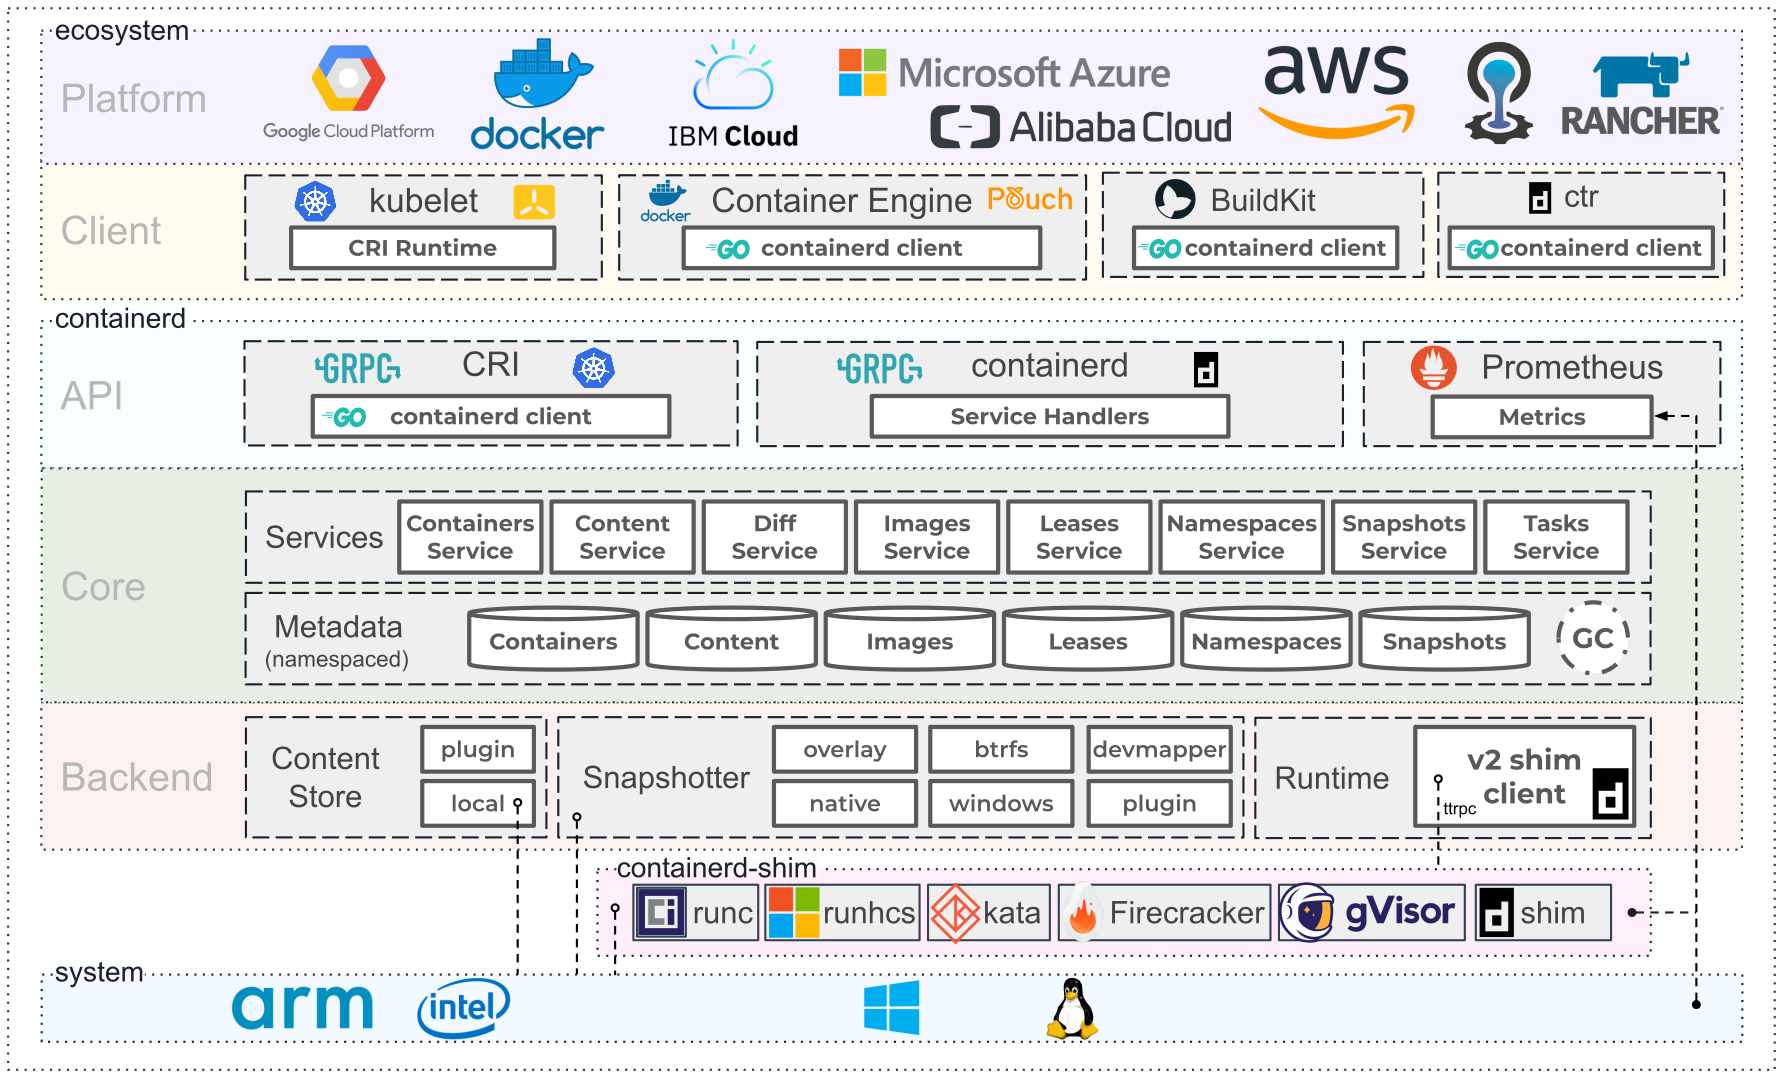
\includegraphics[scale=0.3]{images/software/containerd-architecture.png}
        \caption{A containerd architektúrája \cite{containerdhomepage}}
        \label{containerdarch}
\end{figure}

A konténerek forradalmasították a modern szoftverfejlesztést. De mi is történik valójában a háttérben, amikor egy konténert indítunk? A válasz megértéséhez betekintést kell nyernünk a \texttt{containerd} világába, amely a Docker és a Kubernetes alapjaként szolgált hosszú ideig.

A \texttt{containerd} egy magas szintű konténer futtatókörnyezet, amely az OpenContainers Runtime (OCR) specifikáció szerint működik. Ez a specifikáció határozza meg, hogyan kell a konténereket létrehozni, kezelni és futtatni a különböző platformokon. A containerd nem egyszerűen egy démonfolyamat, hanem egy teljes ökoszisztéma megtestesítője, amely gondoskodik a konténerek teljes életciklusáról, a letöltéstől a futtatásig.

Látni fogjuk, hogy a containerd valójában a konténer ökoszisztéma szíve, amely egységes felületet biztosít a konténerek kezeléséhez, azonban nem olyan magas szintű, mint egy konténer-orchestrációs platform. Nem biztosít például olyan funkciókat, mint a skálázás, a terheléselosztás vagy a szolgáltatásfelfedezés (\textit{service discovery}). Ezeket a funkciókat jellemzően a magasabb szintű orchestrációs platformok nyújtják, mint például a Kubernetes, vagy saját fejlesztésű platformokon a Docker Engine démon.

Az \ref{containerdarch}. ábrán látható a containerd architektúrája, és annak helye a szoftver-ökoszisztémában.

\section{Projektek összeállítása}

% example of docker-compose file, services, networks, etc.

\section{Miben különböznek a Multi-Compose projektek?}

% example of two interconnected compose files

\section{Image-ek frissítési folyamata (sequence diagram)}

\section{Hálózatok összeállítása hagyományos Dockerben}

\section{Hálózatok összeállítása Zebrafishben}

% example of network file : /etc/cni.d

\section{A konténerek közötti függőségek kiszámítása}

% hard dependencie
% soft dependencies

\section{Felhasználói use case-ek (use case diagram + table - pulling images)}

\section{Kliens-szerver architektúra}

\begin{figure}[!h]
	\centering
        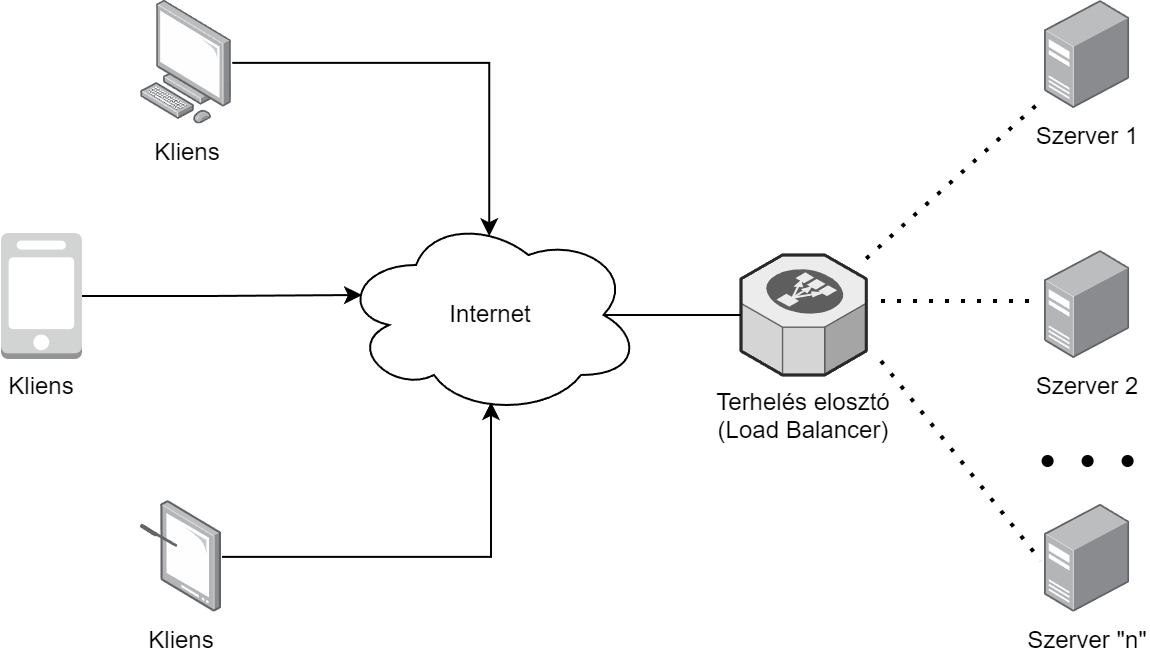
\includegraphics[scale=0.3]{images/software/client-server-arch.png}
	\caption{Tradicionális kliens-szerver architektúra}
        \label{csarch}
\end{figure}

A kliens-szerver architektúrában a felelősségek két kulcsfontosságú komponens - a kliens és a szerver - között oszlanak meg. A kliens-szerver architektúra magába foglalja a \textbf{kliens} fogalmát: egy felhasználóval szemben álló alkalmazást vagy felületet, amely kapcsolatként szolgál a felhasználó és a számítógép között, illetve a \textbf{szerver} fogalmát: egy biztonságos számítógépet, mely elvégzi az adatok feldolgozását.

A kliens és a szerver egy számítógépes hálózaton keresztül kommunikál egymással. A kliensek kéréseket küldenek a szerverek felé, a szerverek pedig a kért információk szolgáltatásával vagy a szükséges feladatok elvégzésével válaszolnak. Ez az architektúra lehetővé teszi a központi vezérlését az adott applikációnak, így alkalmas például webalapú rendszerek kiépítésére.

A Project Raccoon is kliens-szerver architektúrát alkalmaz, még \textit{serverless} környezetben is. A hagyományos telepítések során a Project Raccoon egy központi szerverre van telepítve, amely gondoskodik az API backendről, a frontendről és opcionálisan az adatbázisról és a fájltárolásról is. A szerver nélküli \textit{serverless} telepítések esetén sem beszélünk teljesen szerver \textit{nélküli} architekturáról: a szerver automatikusan elindul, amikor a kliensek információt kérnek a szolgáltatástól.

A \ref{csarch} ábrán látható egy tradicionális kliens-szerver architektúra. A kliensek kéréseket tesznek a szolgáltatás felé. Ezek a kérések átmennek az interneten, amely a kérésüket a terhelés elosztónkhoz (\textit{load balancer}-hez) irányítja, függetlenül attól, hogy a kliensek földrajzilag hol helyezkednek el. 

A \textit{load balancer} feladata, hogy kiossza a beérkező kéréseket a rendelkezésre álló szerverek között. Ez lehetővé teszi a rendszer vertikális skálázását, és megelőzi, hogy bármelyik szerver túlterheltté váljon. A \textit{load balancer} a kérések útbaigazításához több stratégiát vethet be. \cite{loadbalancing} Ezek közül megemlítenék egy párat:

\begin{itemize}
  \item \textbf{Körkörös teherelosztás (\textit{Round-robin balancing})}: Egy egyszerű elvet követ. Körkörösen váltogatja a kiszolgáló szervert a rendelkezésre álló kiszolgálók listájából. Minden új kérést szekvenciálisan a listán következő szerverhez rendelünk, biztosítva ezzel, hogy a munkaterhelés egyenletesen oszlik el az összes rendelkezésre álló erőforrás között. A körkörös terheléselosztás megakadályozza egyetlen kiszolgáló szerver túlterhelését, miközben maximalizálja a rendszer általános teljesítményét és átbocsátóképességét. Ez a megközelítés könnyen megvalósítható, skálázható, és egyszerű módot biztosít a nagy mennyiségű kérések kiegyensúlyozott kezelésére. \cite{loadbalancing}
  \item \textbf{Legkisebb kapcsolaton alapuló tehereloszlás (\textit{Least-connection load balancing})}: Célja, hogy a bejövő kéréseket több az aktuális terhelési szint alapján ossza el. Ez a technika arra törekszik, hogy minimalizálja az egyes kiszolgáló szerverek által kezelt kapcsolatok számát. \cite{loadbalancing} Biztosítja, hogy a munkaterhelés egyenletesen osztódjon el az összes rendelkezésre álló erőforrás között. Amikor új kérés érkezik, a \textit{load balancer} dinamikusan kiválasztja azt a szervert, amelyik a legkevesebb aktív kapcsolattal rendelkezik, és a kérést ehhez rendeli hozzá. Ez minimalizálja a szerver túlterhelésének kockázatát. Ez a megközelítés különösen hatékony olyan esetekben, ahol a szerverek kapcsolatterhelése jelentősen változhat.
  \item \textbf{IP-címen alapú tehereloszlás (\textit{IP hash load balancing})}: A bejövő kérések forrásának IP-címe alapján kiszámít egy hash-értéket, és hozzárendeli azt az egyik elérhető kiszolgálóhoz. A hozzárendelés konzisztens marad az azonos IP-címről érkező későbbi kérések esetében, így biztosítva, hogy egy adott kliens minden kérése ugyanarra a kiszolgálóra irányuljon. Azáltal, hogy a IP-címet használja a terheléselosztás kulcsaként,  biztosítja, hogy a felhasználók munkamenetének késleltetése azonos marad. \cite{loadbalancingtech} Ez különösen létfontosságú a valós idejű alkalmazásoknál, ahol fontos, hogy a késleltetés mértéke egyenletes maradjon. A \textit{Project Raccoon} is tartalmaz valós idejű komponenseket - nevezetesen valós idejű csevegést biztosít az eladó és a vevő között a szerződéstárgyalások során.
\end{itemize}

Nem mindig szükséges terheléselosztó használata, de erősen ajánlott, ha előre látható, hogy nagyon sok felhasználó fogja használni a szolgáltatásunkat. Ha nincs terheléselosztó, akkor a kliensek automatikusan egy központi kiszolgáló szerverhez (\textit{central server}) csatlakoznak. Ebben az esetben a szerverek kiválasztásában nem játszik szerepet terheléselosztó algoritmus, mivel mindig csak egy szerver áll rendelkezésre. Ez azonban különösen veszélyes, mert ha a központi kiszolgáló szerver összeomlik vagy más módon elérhetetlenné válik, nem marad egyetlen kiszolgáló sem, amely a beérkező kéréseket kezelné.

A terheléselosztás különösen fontos, hogy a szolgáltatás leállási ideje (\textit{downtime}) minimális legyen. Ezért a \textit{Project} Raccoon úgy van felépítve, hogy lehetővé tegye a vertikális skálázás használatát. Ez nem feltétlenül szükséges - a \textit{Project Raccoon}-t továbbra is lehet futtatni az összes architekturális többletköltség nélkül, például több adatbázis telepítése, terheléselosztók és több szerver konfigurálása nélkül.

\begin{figure}[!h]
	\centering
        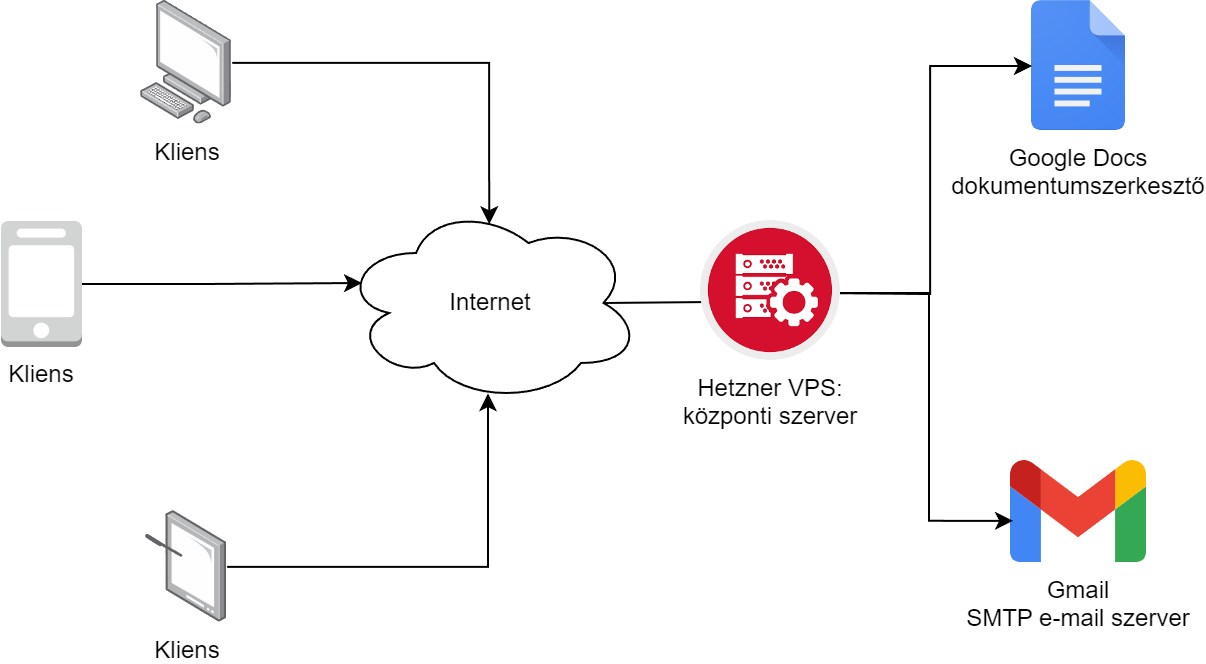
\includegraphics[scale=0.37]{images/software/simplest-architecture.png}
	\caption{A \textit{Project Raccoon} legegyszerűbb kliens-szerver kivitelezése}
        \label{simplestarch}
\end{figure}

A \ref{simplestarch} ábrán látható a \textit{Project Raccoon} legegyszerűbb kitelepítése. Maga a Project Raccoon által szolgáltatott web frontend, API backend, az adatbázisok és a fájltárolás egy Hetzner virtuális számítógép által vannak szolgáltatva. Ebben az esetben a terhelés nincs kiegyenlítve. Ha a Hetzner VPS meghibásodik vagy leáll, a szolgáltatás teljesen elérhetetlenné válik. Megengedhetjük magunknak, hogy az adatbázist és a fájltárolót ezen az egy szerveren hosztoljuk, mert csak ennek az egy szervernek kell hozzáférnie ezekhez.

A \ref{simpleprocon} táblázatban levezetjük ennek a megoldásnak az előnyeit és hátrányait. Mivel ennek a megközelítésnek nagyon erős hátrányai vannak, ajánlott egy bonyolultabb, de nagyobb teljesítményű telepítési architektúrát választani.

\pagebreak

\begin{table}
\begin{tabularx}{\linewidth}{>{\parskip1ex}X@{\kern4\tabcolsep}>{\parskip1ex}X}
\toprule
\hfil\bfseries Előnyök
&
\hfil\bfseries Hátrányok
\\\cmidrule(r{3\tabcolsep}){1-1}\cmidrule(l{-\tabcolsep}){2-2}

Nincs korlátja annak, hogy mit tehetünk a szerveroldalon.\par
A szerver mindig gyorsan válaszol, hiszen nem szükséges külső szolgáltatásokra várakozni.\par
Relatív kevés anyagi erőforrást igényel.\par
Egyszerű felépítése révén könnyen telepíthető és futtatható is.\par
A Docker használatával bármilyen architektúrájú processzorra kitelepíthető, például ARM szerverekre is. \cite{dockerarm}\par

&

Szükséges egy szerver kibérlése, bekonfigurálása és folyamatos üzemeltetése.\par
Nem skálázható vertikálisan - nem tud nagy mennyiségű felhasználót kiszolgálni.\par
Vízszintes skálázás esetén a szerver erőforrásainak kibővítése rendkívül költséges lehet.\par
A telepítés gyakran unalmasabb, és Linux szerver ismereteket igényel.\par
\\\bottomrule
\end{tabularx}
\caption{A legegyszerűbb kivitelezés előnyei és hátrányai}
\label{simpleprocon}
\end{table}

\begin{figure}[!h]
	\centering
        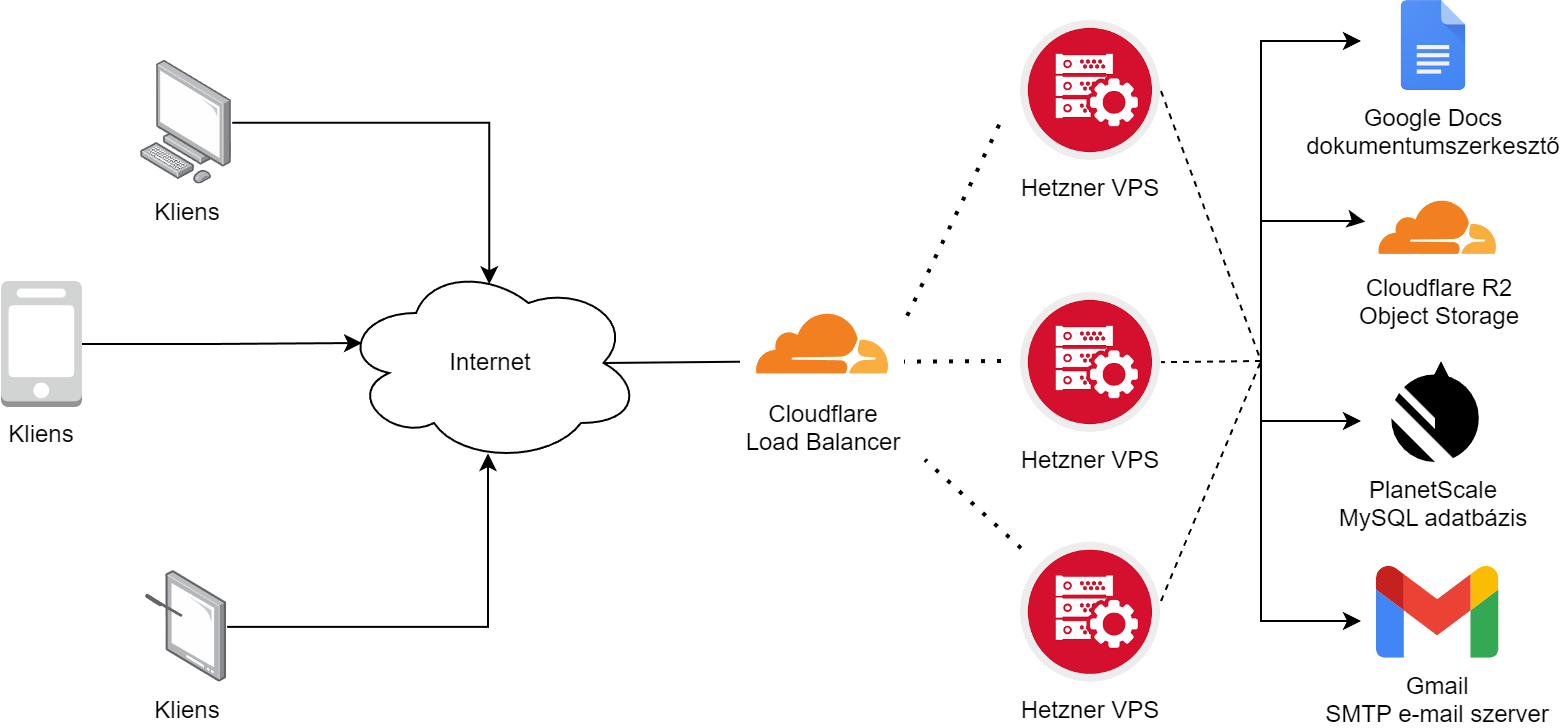
\includegraphics[scale=0.28]{images/software/detailed-arch.png}
	\caption{A \textit{Project Raccoon} részletesebben kidolgozott telepítésének kivitelezése}
        \label{detailedarch}
\end{figure}

A \ref{detailedarch} ábrán látható a \textit{Project Raccoon} részletesebben kidolgozott telepítésének felvázolása. Ebben az esetben is marad a hagyományos szerver-kliens architektúra, hiszen a centralizált szervert felváltja három, egymástól független Hetzner virtuális gép.

Mivel már három különböző szerverről beszélünk, ezért át kell gondoljuk a szerverek hatáskörét. Az előző megvalósításban az adatbázis, illetve a fájlok tárolása egyetlen egy szerveren történt, nem volt szükség külső szolgáltatás használatára. Ebben az esetben viszont szigorúan el kell különítsük a szerverektől az adatokat tárolását. Hogyha az adatokat ugyanazon a szerveren tároljuk, akkor az az adott szerver könnyen túlterheltté váik. Hogyha az adatokat külön-külön minden szerveren tároljuk, akkor redundáns adattárolás történik, sőt, szinkronizálnunk kell az adatokat az összes szerver között, ami egyáltalán nem egyszerű dolog.

Két új szolgáltatást vezetünk be: egy automatikusan önskálázó adatbázis-szolgáltatót, a \textit{PlanetScale}-t illetve a Cloudflare R2 \textit{Object Storage}-t. A \textit{PlanetScale} feladata, hogy a három szerverünk felé szolgáltasson egy olyan adatbázist, amely automatikusan skálázza magát, és bármely időpillanatban elérhető a szerverek számára. A relációs adatbázisunk adatait ebben a rendszerben tárolhatjuk. A három szerver ezentúl nem tárolja saját magában az adatbázis adatait. Hasonlóképpen, a Cloudflare R2 \textit{Object Storage} átveszi a fájltárolás feladatait a Hetzner VPS-től. A Cloudflare R2 centralizált tárolóhelyet biztosít a \textit{Project Raccoon}-nak, lehetőséget adva a rendszernek, hogy itt tárolja a végleges szerződéseket, esetlegesen feltöltött mellékleteket, illetve a felhasználók profilképeit.

A \ref{detailedprocon} táblázatban levezetjük e megoldás előnyeit és hátrányait. Mivel ez a megoldás kevesebb hátránnyal rendelkezik, már alkalmazható huzamosabb ideig, több felhasználó kiszolgálására is.

\begin{table}
\begin{tabularx}{\linewidth}{>{\parskip1ex}X@{\kern4\tabcolsep}>{\parskip1ex}X}
\toprule
\hfil\bfseries Előnyök
&
\hfil\bfseries Hátrányok
\\\cmidrule(r{3\tabcolsep}){1-1}\cmidrule(l{-\tabcolsep}){2-2}

Vertikálisan skálázható, új szerverek hozzáadásával a rendszerben.\par
A szervereket nem terhelik túl a felhasználók kérései.
A Docker használatával egyszerűsíthető a szerverek kitelepítése.\par
Ha megsemmisülnek a szerverek egy hiba során, az adatok megmaradnak a Cloudflare object storage-ban és a PlanetScale adatbázisában.\par
A Cloudflare és a PlanetScale automatikus biztonsági mentéseket végeznek az adatokról.\par

&

Még mindig szükséges a szerverek kibérlése. Mivel több szervert bérlünk, ezért több pénzbe kerül a rendszer futtatása.\par
Nem skálázható vertikálisan - nem tud nagy mennyiségű felhasználót kiszolgálni.\par
Ha nincsen túl sok felhasználónk, nincs értelme egy ennyire komplex kitelepítési architekturát érvénybe léptetni.\par
A telepítés még mindig Linux szerver ismereteket igényel.\par
A PlanetScale adatbázisa kicsit különbözik a megszokott MySQL adatbázisoktól, így fennáll a \textit{vendor lock-in} veszélye. (A vendor lock-in olyan helyzetet jelent, amikor erősen függünk egy adott szolgáltatástól, ami megnehezíti vagy költségessé teszi az alternatív szolgáltatásokra való váltást.)
\\\bottomrule
\end{tabularx}
\caption{A kidolgozott kivitelezés előnyei és hátrányai}
\label{detailedprocon}
\end{table}

\section{Serverless architektúra}

\begin{figure}[!h]
	\centering
        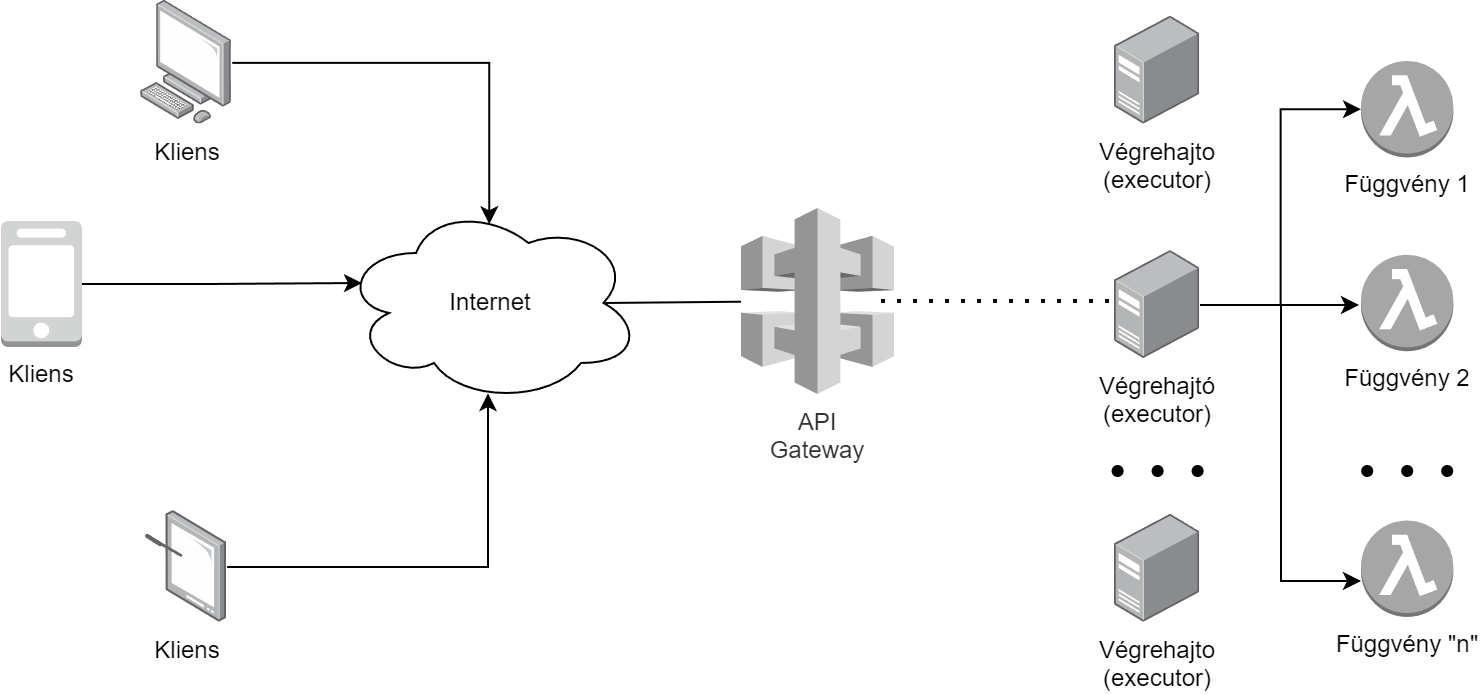
\includegraphics[scale=0.3]{images/software/serverless.png}
	\caption{Kliens-szerver architektúra megvalósítása serverless technológiával}
        \label{serverless}
\end{figure}

A \textit{serverless} architektúra egy felhőalapú modellre utal, ahol az infrastruktúra és a szerver menedzsment feladatai el vannak vonatkoztatva a fejlesztőktől, így azok kizárólag a kód írására és telepítésére koncentrálhatnak. Ez a megközelítés kiküszöböli a szerverek rendelkezésre bocsátásának, konfigurációjának és kezelésének szükségességét, mivel a felhőszolgáltató dinamikusan kezeli a kód végrehajtásához szükséges erőforrásokat. Mivel a \textit{Project Raccoon} alkalmazást a Next.js keretrendszerének kontextusában építettük fel, az alkalmazás teljes mértékben kitelepíthető \textit{serverless} technológiákkal is. A \textit{serverless} technológiák segítségével a \textit{Project Raccoon} kitelepítése egyszerűbbé és skálázhatóbbá válik.

A szerver nélküli kitelepítés stratégiájával a weboldalunk minden egyes elérhetőségét egy külön függvényként kitelepítjük a serverless felhőbe. Ezek a függvények mindig élnek a felhőben, viszont csak akkor futnak, mikor a felhasználók kérik. Mikor egy kérés érkezik egy felhasználó számáról,  a kérés legelőször egy API Gateway-hez kerül. Az API Gateway megkeresi a felhőben lementett függvény lokációját, ahol tárolva van a függvény. Ezután megnézi, hogyha már van olyan szerver a felhőben, amely jelenleg futtatja az adott függvényt. Ha van, a kérést ahhoz a szerverhez továbbítja, ahol a kért függvény fut. Ha nincs, akkor keres egy olyan szervert, amely nincs túlságosan lefoglalva kérésekkel. A kapott szerver letölti a felhőből a függvény forráskódját, és elkezdi futtatni. Ezt nevezik hidegindításnak (angolul: \textit{cold boot}). Sajnos ez enyhe késleltetést eredményez az olyan alkalmazások esetében, amelyeket egy ideje nem használt egyetlen felhasználó sem. A hideginditás után, ha az alkalmazást nem használja huzamosabb ideig egyetlen felhasználó sem, a függvény lekapcsolódik és új kérés esetén újra szükségessé válik egy új szerver keresése és a függvény újratelepítése (mégegy hidegindítás szükséges). \cite{serverlessbib}

A Project Raccoon esetében a \textit{serverless} technológiákkal való kitelepítést a Vercel platform használatával ajánljuk. Mivel a Next.js keretrendszert a Vercel készítette, ezért nyílvánvaló, hogy a Next.js teljes mértékben fel van szerelve a \textit{serverless} technológiák támogatására. A \textit{serverless} telepítés során ugyancsak szükséges az alkalmazás összekötése a Google Docs, Cloudflare R2, PlanetScale és Gmail rendszerekkel. A Cloudflare Load Balancer szerepét lecseréli a Vercel API gatewayje, amely a Vercel hálózatában automatikusan kiosztja a szerver nélküli függvények a kiszolgáló szerverek között. Nincs szükség saját szerver futtatására, karbantartására.

A \ref{serverlessprocon} táblázatban a \textit{serverless} megközelítés előnyeit és hátrányait tárgyaljuk. Ez a megközelítés olyan esetben megfelelő, amikor vagy alig felhasználó, és nincs igazi oka egy teljes szerver felállításának, vagy akkor, amikor olyan sok felhasználó van, hogy nagyon nehéz lenne egy egész szervercsoportot (\textit{server cluster}-t) kezelni.

\begin{table}
\begin{tabularx}{\linewidth}{>{\parskip1ex}X@{\kern4\tabcolsep}>{\parskip1ex}X}
\toprule
\hfil\bfseries Előnyök
&
\hfil\bfseries Hátrányok
\\\cmidrule(r{3\tabcolsep}){1-1}\cmidrule(l{-\tabcolsep}){2-2}

Könnyű telepítés és skálázhatóság\par
Kevesebb időtöltés szerverek beállításával\par
Nem szükségesek a Linux szerver adminisztráció lépéseinek ismerete.\par
Nincs szükség külön szerverre - minden a szerver nélküli funkciókon fut a felhőben.\par
Kevés felhasználó esetén sokkal olcsóbb a szolgáltatás serverless futtatása, mint a szerver bérlése.\par

&

A serverless szolgáltató által előírt összes korlátozás érvényesek.\par
Egy esetleges DDoS (\textit{Distributed Denial of Service}) támadás során a szolgáltatás működtetésének költségei az egekbe szökhetnek, nagy anyagi károkat okozva.\par
A hidegindítások nagyon lassúvá teszik a kapcsolat létesítését a szolgáltatással, ha hosszabb ideig nem használják.\par

\\\bottomrule
\end{tabularx}
\caption{A serverless kivitelezés előnyei és hátrányai}
\label{serverlessprocon}
\end{table}

\pagebreak

\section{MVC - Modell-Nézet-Vezérlő}

A \textit{Project Raccoon} keretén belül az MVC szoftver architektúrális mintát használjuk. Az \textbf{MVC} - Modell-Nézet-Vezérlő minta megengedi nekünk, hogy a kódbázisunkat moduláris modulokból építsük fel.

A modell képviseli az alkalmazás adatait és üzleti logikáját, és kezeli az adatbázisokkal és külső szolgáltatásokkal való adatinterakciókat. A nézet (\textit{view}) kezeli az adatok megjelenítését a felhasználók számára, felhasználói felületét jelképezve a szoftvernek. A modell és a nézet közötti hídként működő Vezérlő kezeli a felhasználók kéréseit, dolgozza fel az adatokat, és ennek megfelelően frissíti a modellt és olykor a nézetet. A felelősségek egyértelmű szétválasztása ily módon megkönnyíti a kód karbantartását.

\subsection{Modellek}

A \textit{Project Raccoon} az adatok modellezésére a TypeORM keretrendszert használja. A TypeORM keretén belül a TypeScript-el megírt osztályok automatikusan leképezhetőek relációs és nem-relációs adatbázisokra is egyaránt. A relációs adatbázis sémák metaadatait, mint több más hasonló keretrendszerben is, a modellekben megadhatjuk dekorátorok segítségével. Minden modellünk két részből áll:

\begin{enumerate}
  \item egy \textbf{interfészből}, amely meghatározza az entitás adattaigjait egy általános, nem TypeORM-specifikus módon - lásd \ref{code:modelinterface} kódrészlet;
  \item illetve egy \textbf{TypeORM entitásból}, amely implementálja az interfészt, TypeORM-specifikus és metaadatokat is tartalmaz dekorátorok formájában - lásd \ref{code:modelentity} kódrészlet.
\end{enumerate}

\begin{lstlisting}[caption={ Egy modell interfészének megvalósítása }, captionpos=b, language = TS, label={code:modelinterface}]
export interface IItem {
  id?: number;
  createdAt?: Date;
  updatedAt?: Date;
  friendlyName?: string;
  slug?: string;
  description?: string;
  options?: IItemOption[];
}
\end{lstlisting}

\pagebreak

\begin{lstlisting}[caption={ Egy modell entitásának megvalósítása }, captionpos=b, language = TS, label={code:modelentity}]
@Entity()
export class Item implements IItem {
  @PrimaryGeneratedColumn()
  id: number;

  @CreateDateColumn()
  createdAt: Date;

  @UpdateDateColumn()
  updatedAt: Date;

  @DeleteDateColumn()
  deletedAt?: Date;

  @Column()
  friendlyName: string;

  @Column({ unique: true })
  slug: string;

  @Column()
  description: string;

  @OneToMany(() => ItemOption, (itemOption) => itemOption.item)
  options: Partial<ItemOption[]>;
}
\end{lstlisting}

\subsection{Nézetek}

A \textit{Project Raccoon}-ban a nézetek React komponenseknek felelnek meg. Hosszú csata folyik a React programozók között. Néhányan a régi, osztályalapú megközelítést részesítik előnyben a React felhasználói felület komponensek létrehozásakor, míg mások az újabb, funkcionális megközelítést szeretik jobban. Mi a funkcionális komponensek mellett döntöttünk. Ez azt jelenti, hogy ahelyett, hogy minden React nézetet egy osztályként hozunk létre, helyette minden nézet egy-egy függvénynek írunk meg. Ezért nem is tudunk szolgáltatni hagyományos osztálydiagrammal.

Az osztály-alapú nézetek és a funkcionális nézet között a legnagyobb különbség, hogy míg az osztály-alapú nézetekben explicit módon meg kell határozni az állapotváltozókat és minden más adatforrást, a funkcionális komponensek esetén használható a függőség befecskendezés fogalma (angolul: \textit{dependency injection}), lásd: \ref{code:depinj}. kódrészlet.

\begin{lstlisting}[caption={ A felhasználó objektum befecskendezése egy React komponensbe }, captionpos=b, language = TS, label={code:depinj}]
const LoginForm = () => {
  const [user, setUser] = useCurrentUser();

  if (user) {
    return <p>You are already logged in as {user.username}!</p>;
  }

  return (
    <form>
      ...
    </form>
  );
}
\end{lstlisting}

\subsection{Vezérlők}

A \textit{Project Raccoon} rendszeren belül csupán a vezerlők képesek módosítani közvetlenül a modelleken. A vezerlők a \textit{controllers} mappában élnek, és entitás szerint csoportosítva vannak. Minden egyes vezérlő minden egyes függvényére hivatkozik egy API route a \textit{pages/api} mappából.

A \textit{next-bar} csomag használatával a \textit{pages/api} mappában meghatározhatunk API útvonalakat (\ref{code:apiroute}. kódrészlet). Ezek az API útvonalak a HTTP metódus típusa alapján kerülnek kiválasztásra, mint például POST, GET, DELETE stb.

\pagebreak

\begin{lstlisting}[caption={ Példa implementáció egy API útvonalra, mely egy vezérlőre csatlakozik }, captionpos=b, language = TS, label={code:apiroute}]
import bar from 'next-bar';
import { ensureAdministrator } from '@/middleware/auth';
import * as contractOptionsController from '@/controllers/contract-options/contractOptionsController';

export default bar({
  post: ensureAdministrator(contractOptionsController.newContractOption),
  get: ensureAdministrator(contractOptionsController.listContractOptions),
});
\end{lstlisting}

Ez esetben a vezérlő a \textit{controllers/contract-options/contractOptionsController.ts} állományban él. Két függvényt tartalmaz. Az egyik függvény egy POST hívásra létrehoz egy új szerződés sablon opciót, a másik függvény pedig egy GET hívásra kilistázza az összes szerzdős sablon opciót. A vezérlő feladata, hogy kiolvassa a HTTP kérésekből a szükséges információkat, és hogy hajtsa végre a kért műveletet. Abban az esetben, hogyha olyan megszorítások vannak egy API útvonalra, amelyek nem teljesülnek, a kérés nem hajtódik végre. A \ref{code:apiroute}. kódrészletben például mindkét funkcionalitás csak akkor érhető el, hogyha a felhasználó adminisztrátor felhasználó.

Fontos megemlíteni, hogy a fő vezérlő fájlokban csupán a HTTP kérések feldolgozása hajtódik végre. Minden üzleti logikát, aszerint, hogy mit hajt végre, külön fájlban implementáltunk ugyanabban a modulban. Ez esetben például a ``\textit{newContractOption}'' függvényhez tartozik egy \textit{controllers/contract-options/newContract.ts} állomány is, amely végrehajta a szószerinti üzleti logikát.

\section{Szolgáltatási réteg}

A felhasználói felület a HTTP-kéréseket nem közvetlenül a felhasználói felületből indítja, hanem a szolgáltatási rétegnek delegálja. A szolgáltatási réteg a \textit{Project Raccoon} azon modulja, amely a fejlesztőtől elabsztraktizálja a HTTP kérések logikáját, és az entitásokhoz tartozó szolgáltatásokban gondolkozik. Amikor a felhasználói felületnek egy műveletet kell végrehajtania, vagy adatokat kell kérnie az API-tól, az adott entitásért felelős szolgáltatással lép kapcsolatba, ahelyett, hogy magára HTTP-kérést intézne. Ez nagyon megkönnyíti egy stabil API létrehozását, amelyet nagyon nehéz helytelenül használni, mivel az összes API-specifikus kommunikációt különálló modulokba szét lehet választani és külön-külön tesztelni lehet.

\section{Szerződéssablonok létrehozása}

\begin{figure}[!h]
	\centering
        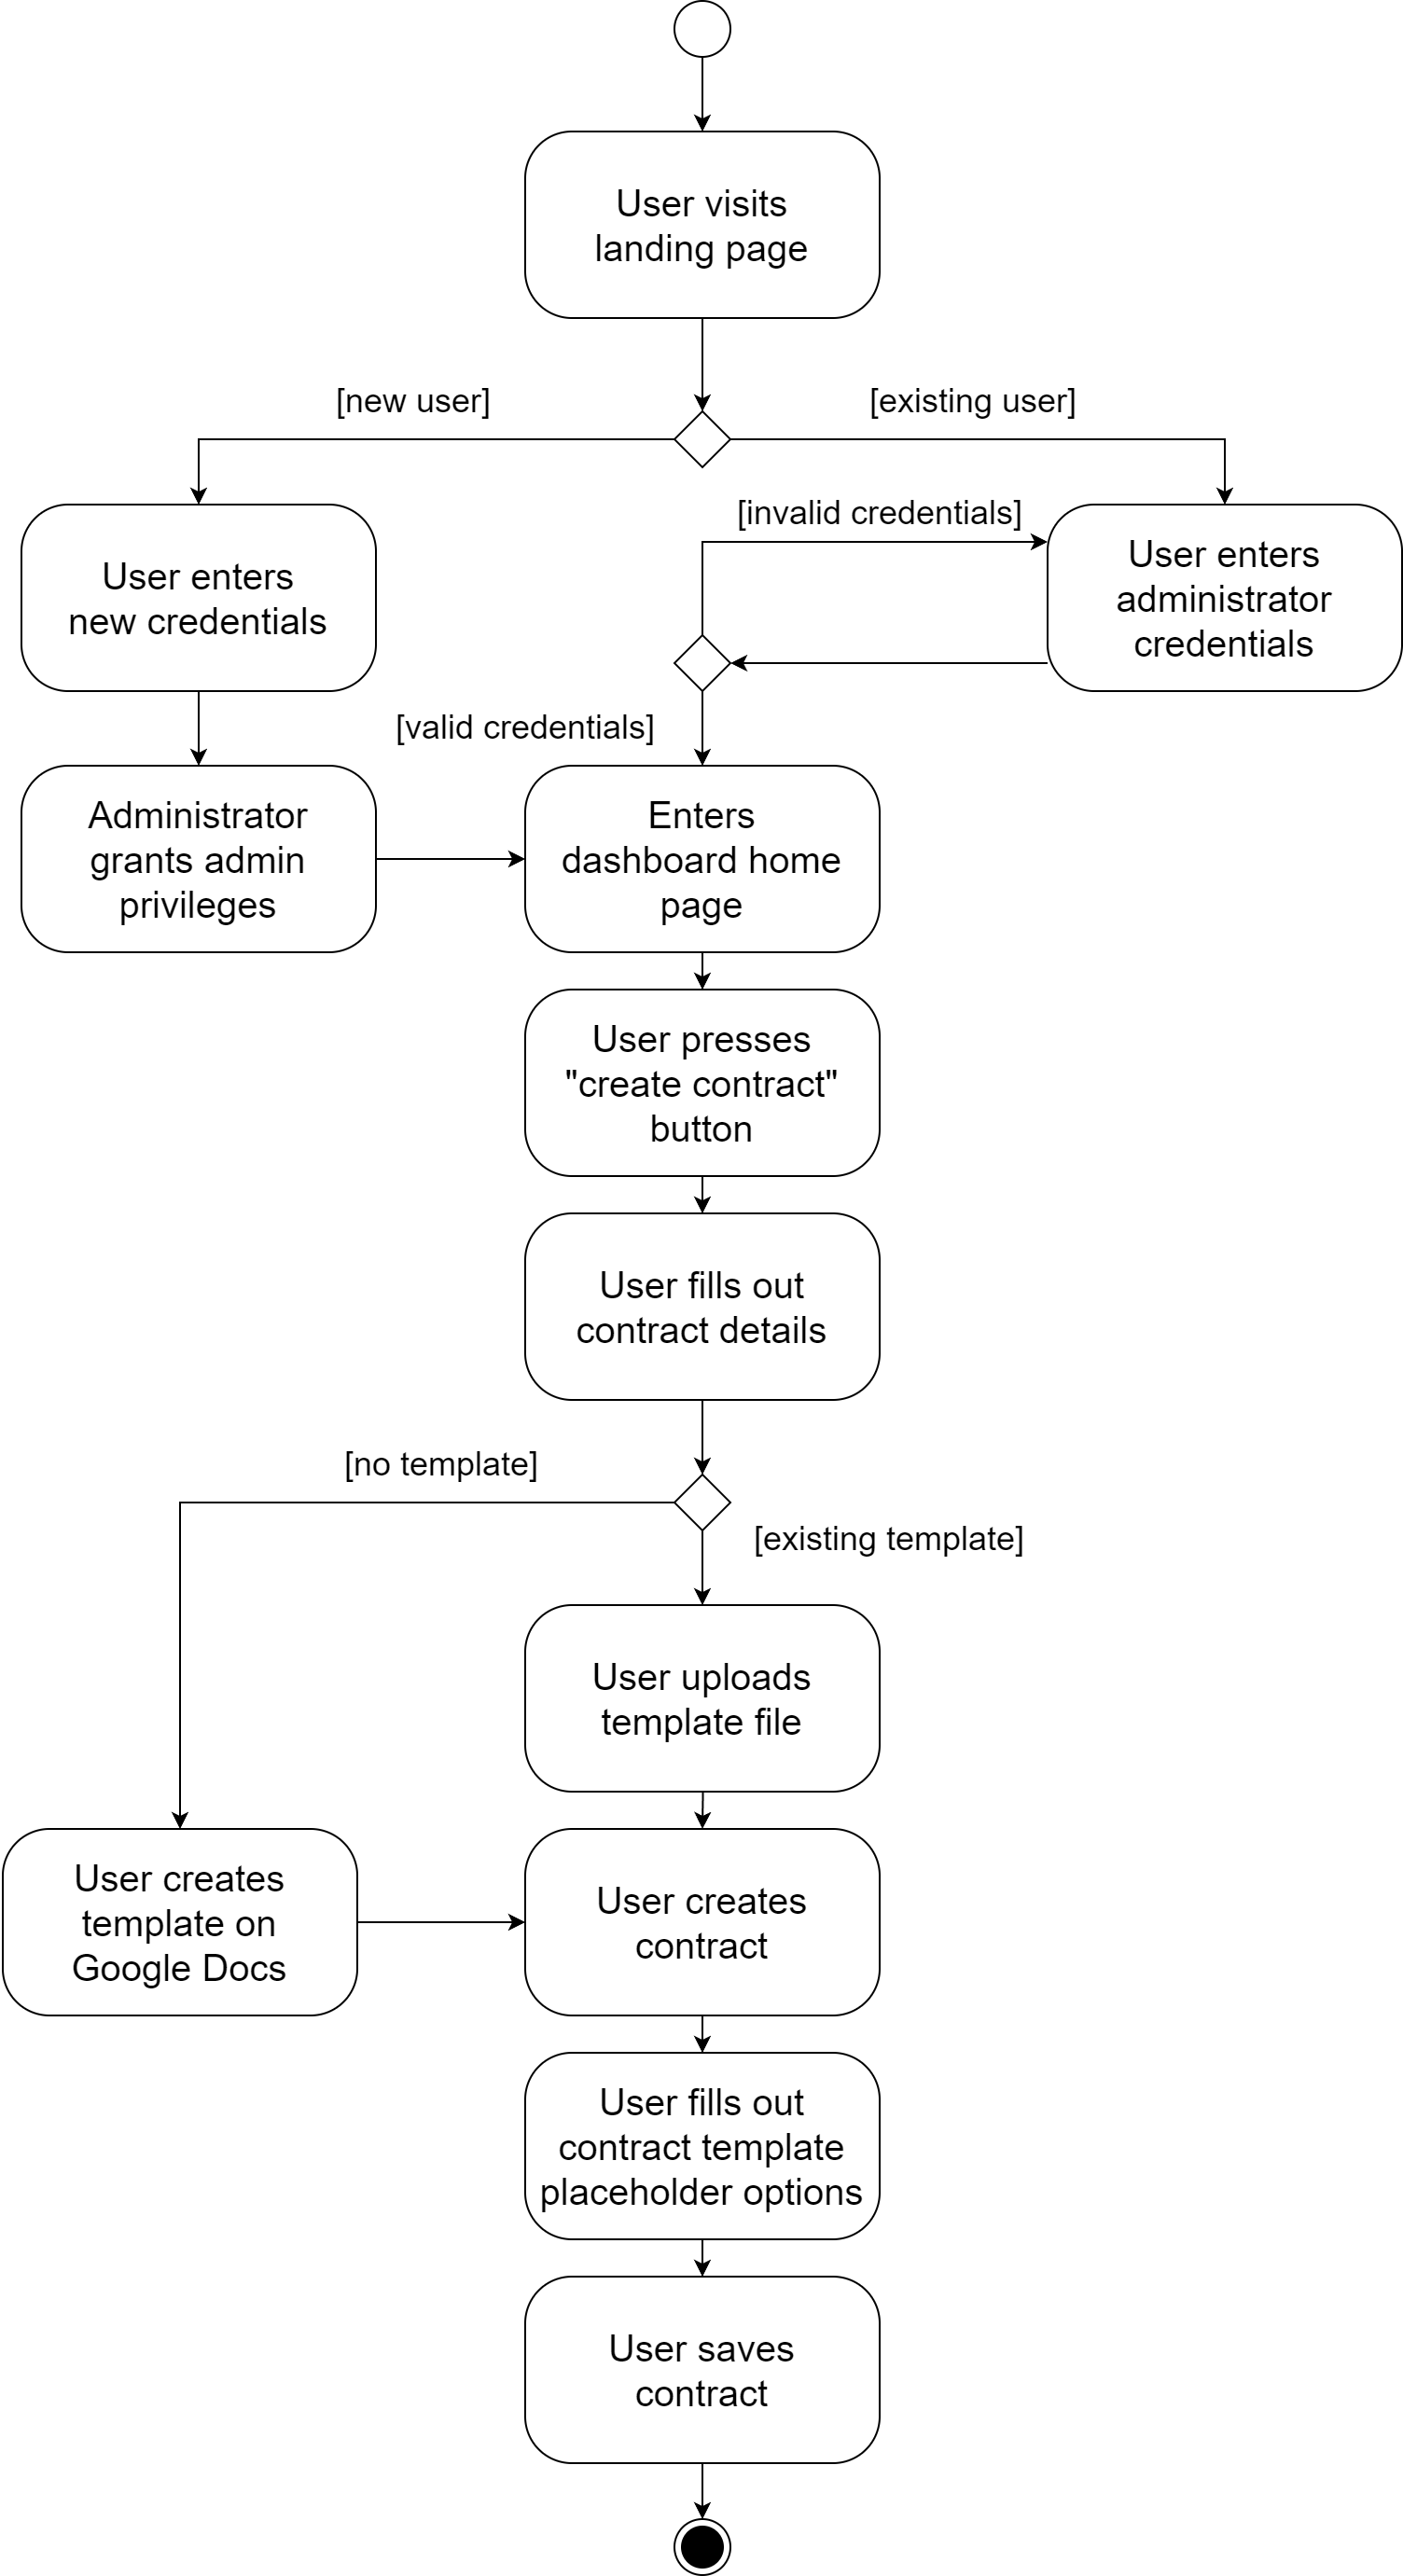
\includegraphics[scale=0.2]{images/software/activity.png}
	\caption{A szerződések létrehozásának activity diagramja}
        \label{software:activity}
\end{figure}

A \ref{software:activity}. ábrán látható a szerződések létrehozásának activity diagramja. A tevékenység kezdetén a felhasználó meglátogatja a weboldal főoldalát.

A weboldal főoldalából két lehetőség nyílik a felhasználó fele: Ha a felhasználó már rendelkezik egy adminisztrátor fiók hitelesítési adataival, akkor beírhatja ezeket a hitelesítési adatokat. Hogyha a rendszer helyesnek véli ezeket az adatokat, akkor továbbengedi a műszerfal kezdőlapjára. Ha viszont a rendszer helytelennek gondolja a hitelesítési adatokat, a felhasználó újból be kell írja azokat.

Ha nincsen adminisztrátor fiókja a felhasználónak, akkor létrehoz egy új fiókot, új hitelesítési adatok megadásával. A hitelesítési adatok megadása után megvárja, hogy egy másik adminisztrátor adminisztrátor jogokkal ruházza fel őt. Ezután kerül át a felhasználó a műszerfal kezdőlapjára.

Miután a felhasználó a műszerfal kezdőlapján van, rákattint a "Szerződés létrehozása" gombra. Ezután kitölti a szerződés sablon összes részletét. Hogyha a felhasználó már készült egy előre elkészített sablonnal, akkor feltöltheti azt. Ha nem készült már előre elkészített sablonnal, akkor a felhasználó létrehoz egy új, üres sablont a Google Docs-ban.

Miután létrejött a dokumentum sablonját, a felhasználó létrehozza a szerződéstípust. A szerződéstípus létrehozása után a felhasználó kitölti az összes olyan űrlapopciót, amelyet a felhasználó megváltoztathat, és amely a Google Docs rendszerben létrehozott dokumentumsablonon megtalálható.

Az űrlapopciók létrehozása után a felhasználó lementi a szerződés típusát, a folyamat végére érve.

\pagebreak

\section{Végleges szerződések kigenerálása}

\begin{figure}[!h]
	\centering
        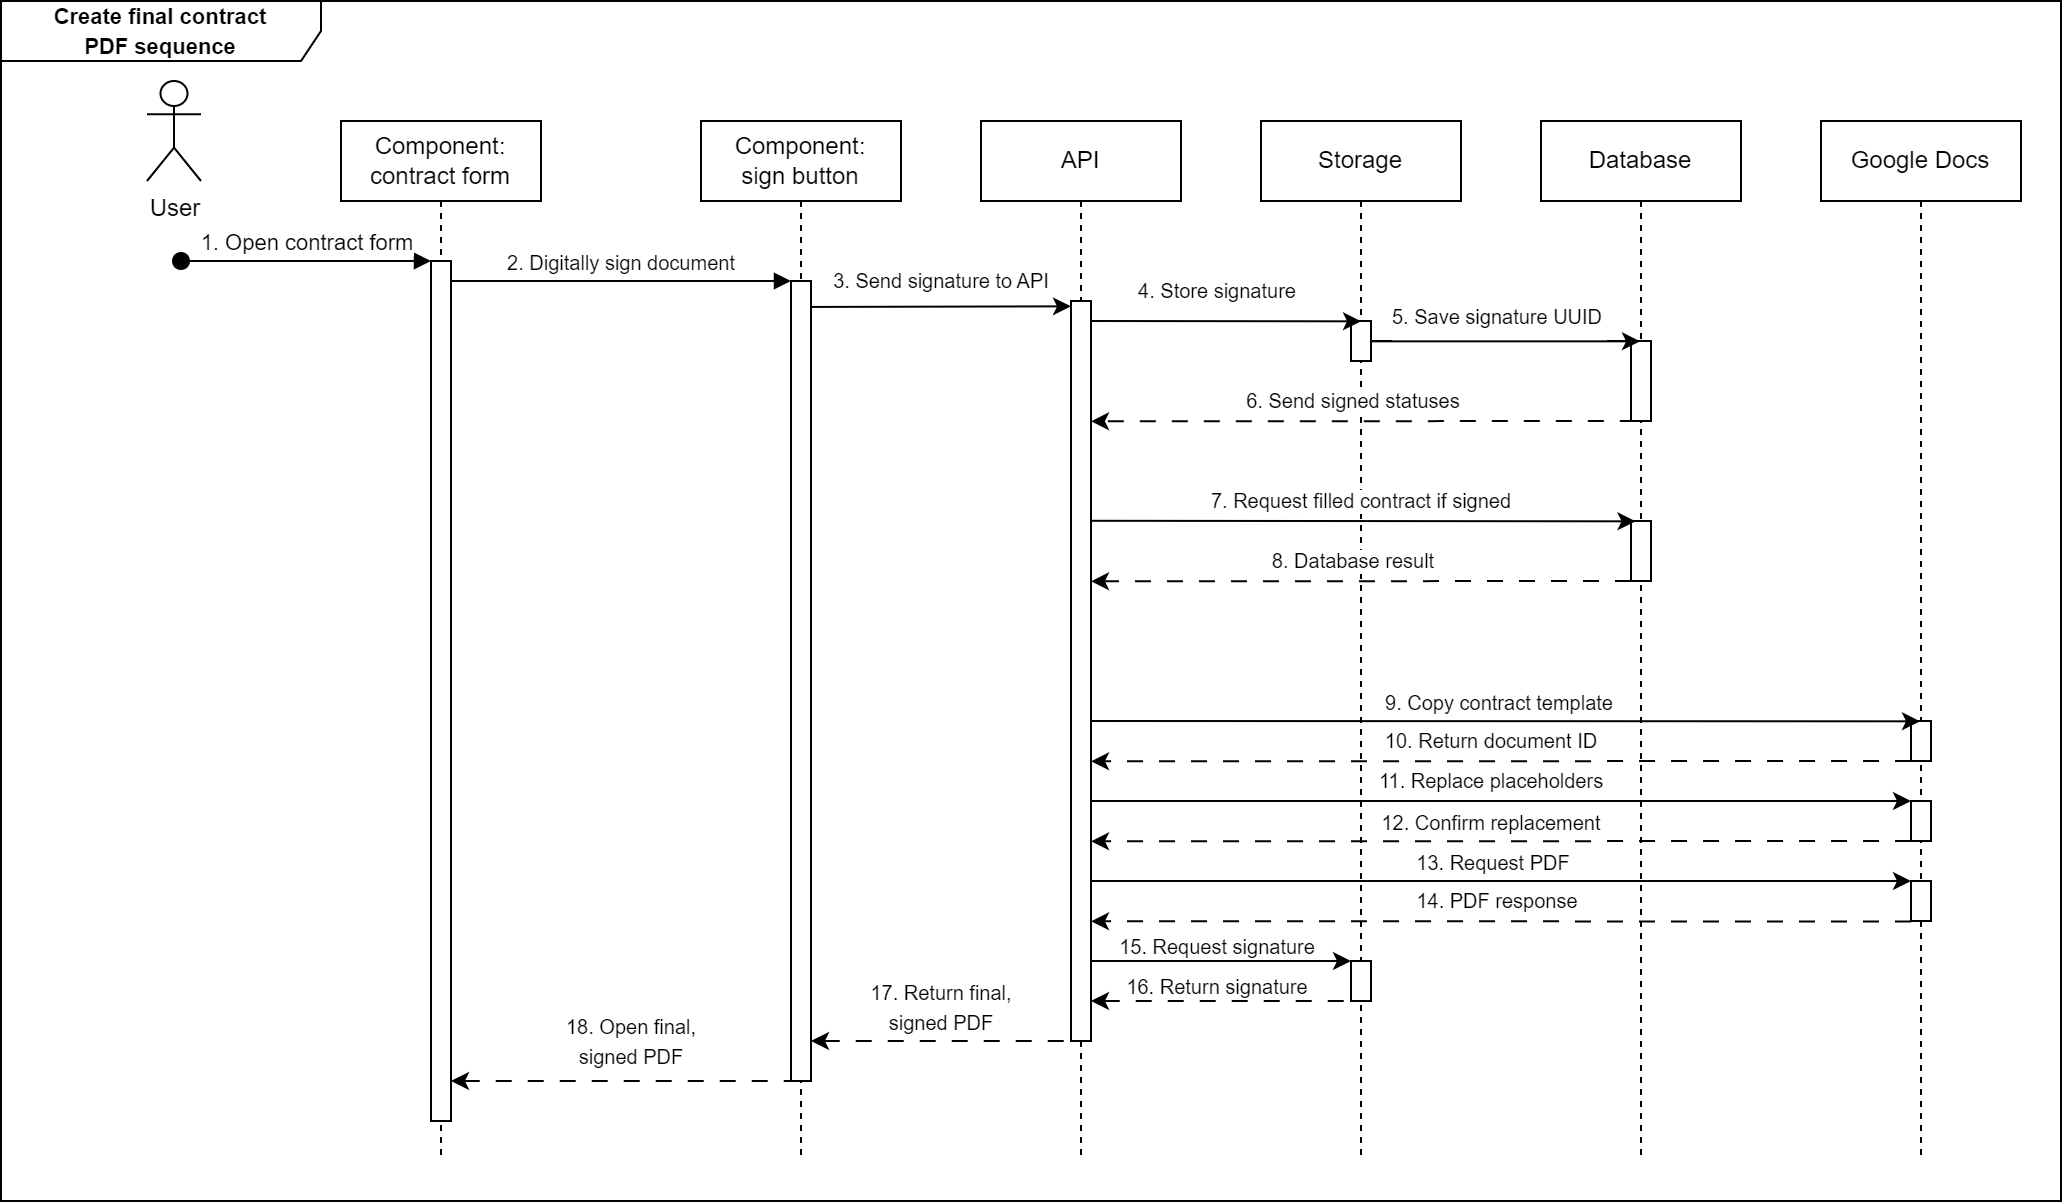
\includegraphics[scale=0.22]{images/software/sequence.png}
	\caption{A végleges szerződések kigenerálásának szekvencia diagramja}
        \label{software:sequence}
\end{figure}

A \ref{software:sequence} ábrán látható a végleges szerződések kigenerálásának szekvencia diagramja. Ebben a szekvenciában hét alkomponens játszik szerepet: maga a felhasználó, a szerződés űrlapja, az aláíró gomb, az API backend, a háttértároló, az adatbázis illetve a külső Google Docs rendszer.

A folyamat elején a felhasználó kinyitja a szerződés űrlapját, és a szerződés űrlapján rákattint az aláíró gombra. A dokumentum így digitális aláírásra kerül. Az aláíró gomb elküldi a digitális aláírást az API számára, amely továbbküldi azt a háttértárolónak. A háttértároló kigenerál egy egyetemesen egyedi azonosítót, ami jellemzi az adott digitális aláírást, és elküldi az adatbázisnak. Az adatbázis visszatéríti az API-nak, hogy mely felhasználók írták eddig alá a szerződést és melyek nem.

Ha az összes felhasználó aláírta a szerződést, akkor folytatódik a végleges szerződés kigenerálása. Az API kér egy másolatot a szerződés sablonáról a Google Docs rendszertől. A Google Docs visszaszolgáltatja az új másolat azonosítóját. Az API ezután összegyűjti az összes űrlap elemet, amelyet helyettesíteni szeretne a dokumentumon. Ezeket a helyettesíteket kötelegelve elküldi a Google Docs rendszernek. A Google Docs visszaküldi a kicserélt űrlapelemek számát az API-nak. Ezután az API megkéri a Google Docs rendszertől, hogy generáljon egy PDF dokumentumot. A Google Docs rendszer visszatéríti az API-nak a kitöltött PDF dokumentumot.

A kitöltött PDF dokumentum még nincs aláírva. Az API lekéri a háttértárolóból a digitális aláírásokat. A háttértároló visszaszolgáltatja az API-nak ezeket az aláírásokat. Az API beszúrja a PDF dokumentumba a \textit{pdf-lib}
és \textit{node-signpdf} könyvtárak segítségével a digitális aláírásokat, kigenerálja az AVDH tanúsítványokat, és visszatéríti a végleges, digitálisan aláírt PDF állományt az aláíró gombnak, ahonnan visszakerül a szerződési űrlapra, és kinyílik a felhasználó számára, hogy megtekintse.

\section{Felhasználói felület tervezése}

\begin{figure}[!h]
	\centering
        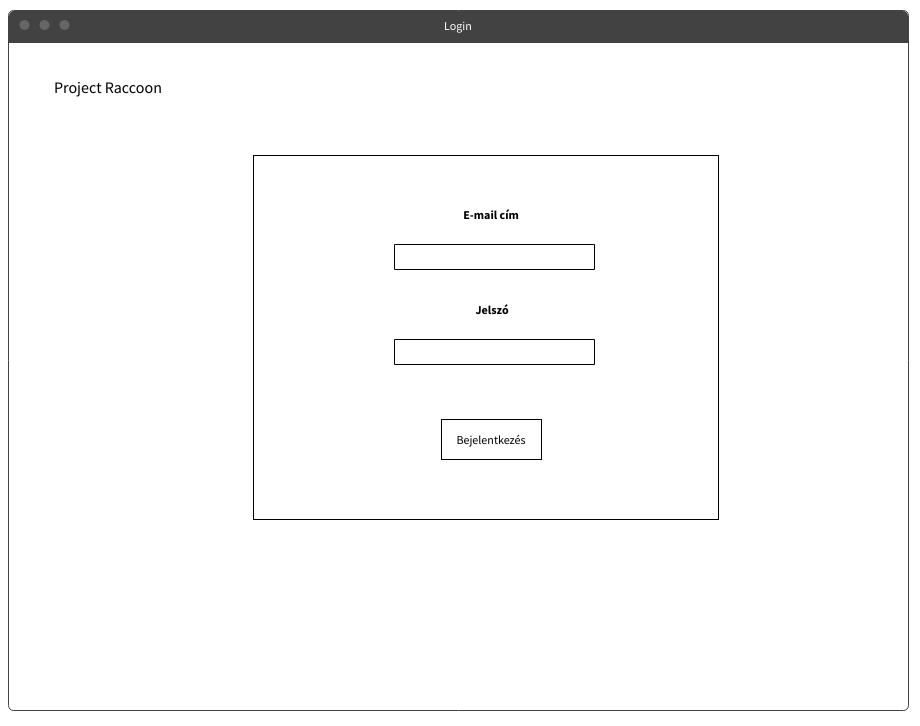
\includegraphics[scale=0.5]{images/wireframe/login.png}
	\caption{A Project Raccoon belépési felületének drótváza}
        \label{wireframe:login}
\end{figure}

A következőekben a tervezés során kialakított drótvázról (\textit{wireframe}) lesz szó. Ezen \textit{wireframe}k segítségével átfogó képet kaphatunk a felületek kinézetéről, az elemensek elhelyezkedéséről, egymáshoz való viszonyulásáról és méretéről. Mindezt anélkül, hogy az apró részletek, színek elhomályosítanák ezen nagyobb körvonalakat. A tervezés során elsődleges szempont volt a felület könnyű használhatósága, az átláthatóság és a reszponzivítás. A folyamat során igyekeztünk betartani Nielsen által felsorolt heurisztikákat \cite{nielsen2005ten} a felület minél nagyobb fokú használhatóságának érdekében. 

\begin{figure}[!h]
	\centering
        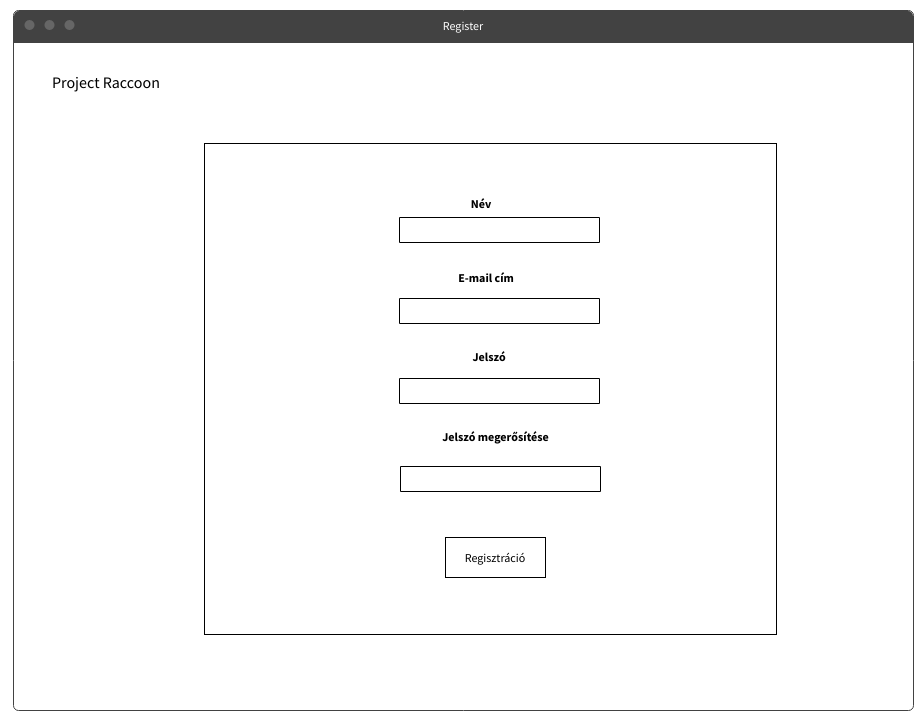
\includegraphics[scale=0.5]{images/wireframe/register.png}
	\caption{A Project Raccoon regisztrációs felületének drótváza}
        \label{wireframe:register}
\end{figure}

Tekintsünk meg néhány fontosabb oldal \textit{wireframe}jét. A bemutatott dizájn az átlagfelhasználók szemszögéből fogja bemutatni a weboldalt (tehát eltekintünk most az adminisztrátori jogkörrel ellátott felhasználóktól). Legelsőnek a \ref{wireframe:login}. ábrán láthatjuk a bejelentkezési oldal drótvázát, amely egyszerűen csak a felhasználót hitelesítő adatok beírása végetti szövegdobozokat és a belépéshez szükséges gombot tartalmazza középre igazítva. A belépéshez egy email cím és egy jelszó szükséges. Miután a felhasználó ezeket beírta, a ``Bejelentkezés'' gombra kattintva be tud lépni a platformra és megtekintheti a saját \textit{dashboard}ját.

Amennyiben a felhasználó nem rendelkezik fiókkal, regisztrálhat a regisztrációs felületen, amely a következőképp néz ki (\ref{wireframe:register}. ábra). A felület tartalmaz négy szövegdobozt, amelybe a felhasználó beírhatja adatait ezek rendre a következőek: név, email cím, jelszó és a jelszó újbóli beírása - az elgépelések kivédéséért fontos. Ezután pedig egy ``Regisztráció'' gomb következik a beírt szövegek elküldése és a regisztráció finalizálása végett. 

\begin{figure}[!h]
	\centering
        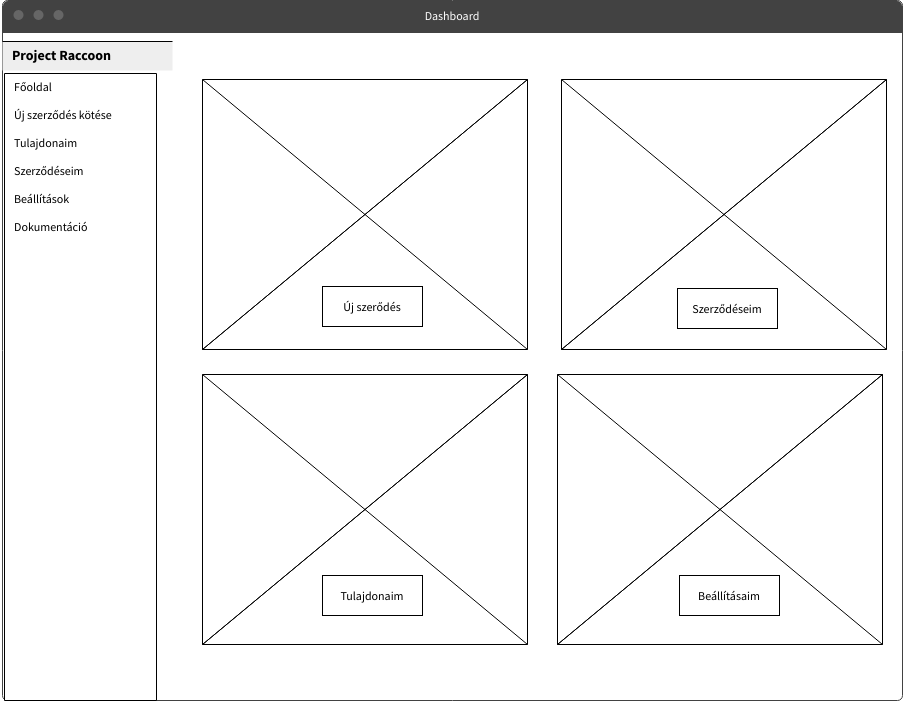
\includegraphics[scale=0.5]{images/wireframe/dashboard.png}
	\caption{A Project Raccoon \textit{dashboard}jának drótváza}
        \label{wireframe:dashboard}
\end{figure}

Sikeres regisztráció után a felhasználó be tud lépni a bejelentkezési felületen. Miután ez megtörtént, megtekintheti a \textit{dashboard}ját, amely a tervezési fázisban a következőképp nézett ki. Ezt a \ref{wireframe:dashboard}. ábra is szemlélteti. Bal oldalt található egy menü, amely segítségével a felhasználó navigálhat a weboldalon: létrehozhat új szerződést, megtekintheti a tulajdonait, valamint a szerződéseit. Különböző beállításokat végezhet, mint például: adatai módosíthatja, vihet be új adatokat, amelyek szükségesek lehetnek a szerződések kitöltése érdekében, de nem voltak elkérve a regisztráció során (anyja születési neve, személyi igazolványának száma, lakhelye stb.). Illetve megtekintheti a platform dokumentációját, vagyis a súgót (használati kézikönyv) - ha bármilyen problémája akad a felhasználónak az oldal használata közben, többek között könnyedén megkeresheti a megoldást/informálódhat ebből is. Ez növeli a felhasználók kényelmét, és az önálló használatot. Tanulmányok már 2013-ban kimutatták, hogy az emberek szívesebben választanak önálló segítségkérési lehetőségeket, mintsemn emailt írjanak, hívást kezdeményezzenek egy ügyfélszolgálattal, illetve, hogy ``a felhasználók 70\% elvárja, hogy egy portálon igénybe tudjanak venni olyan segítséget, amelyhez nem kell más ember beavatkozása'' \cite{van2013self}. Végezetül pedig egy ``Főoldal'' menüpont is szerepel, amely visszavisz a \textit{dashboard}ra. A navigációs menü felett található a platform neve is, amely megjelenik ugyanúgy belépéskor és regisztrációkor is. Jelenleg ezt egy egyszerű \textit{``Project Raccoon''} felirat szemlélteti. 

Középre helyezve pedig megtalálhatóak ugyanezek a főbb alpontok, csupán nagyban kiemelve, hogy még szembetűnőbbek legyenek a felhasználók számára.  

\begin{figure}[!h]
	\centering
        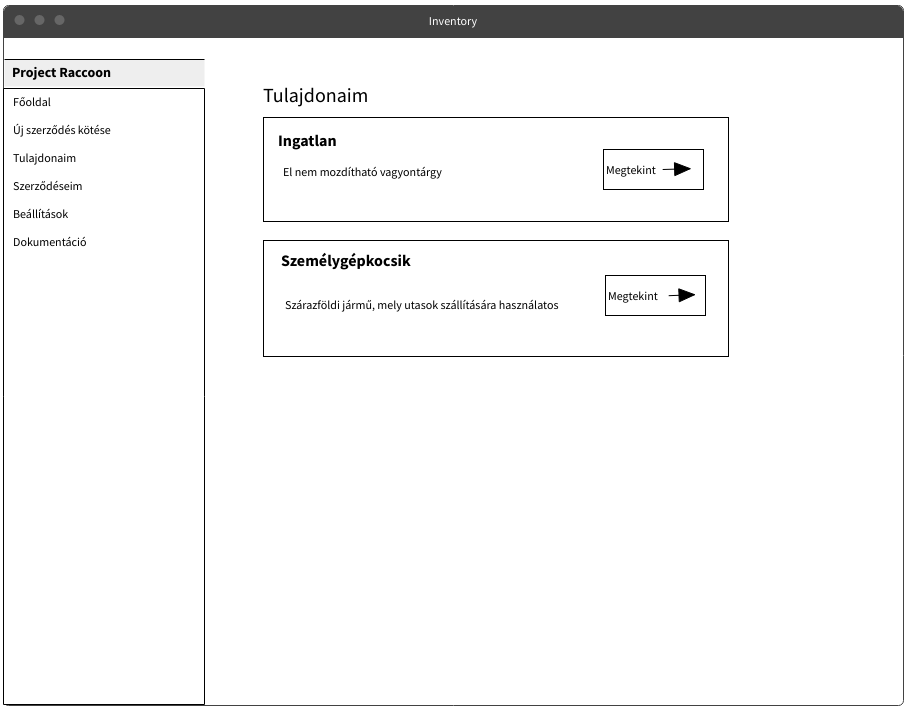
\includegraphics[scale=0.4]{images/wireframe/inventory.png}
	\caption{A Project Raccoon tulajdonokat (kategóriánként) megjelenítő felületének drótváza}
        \label{wireframe:inventory}
\end{figure}

A következő \ref{wireframe:inventory}. ábrán a ``Tulajdonaim'' oldalt láthatjuk, amely a portál adatbázisába felvitt ingó és ingatlanokat listázza. Oldalt a már elmagyarázott navigációs menü található, középül pedig a két kategóriára osztott tulajdonok. Ezek megnevezései alatt egy rövid leírás található az adott katergóriáról, illetve egy-egy gomb, ami még részletesebb megtekintését/listázását adja az adott tulajdonoknak.

A fontosabb wireframek közül utolsónak a szerződéseket listázó oldalt tekintsük meg. A \ref{wireframe:contracts}. ábra ezt szemlélteti. Bal oldalt a fentebb elmagyarázott navigációs sáv található, középül pedig a szerződések típusai szerint kategóriákra osztva láthatjuk és menedzserelhetjük a szerződéseinket. Ezalatt értjük új szerződések kitöltését/létrehozását, amelyet a kategórián belüli ``Új szerződés kitöltése'' gombra kattintva meg is tehet a felhasználó.

\begin{figure}[!h]
	\centering
        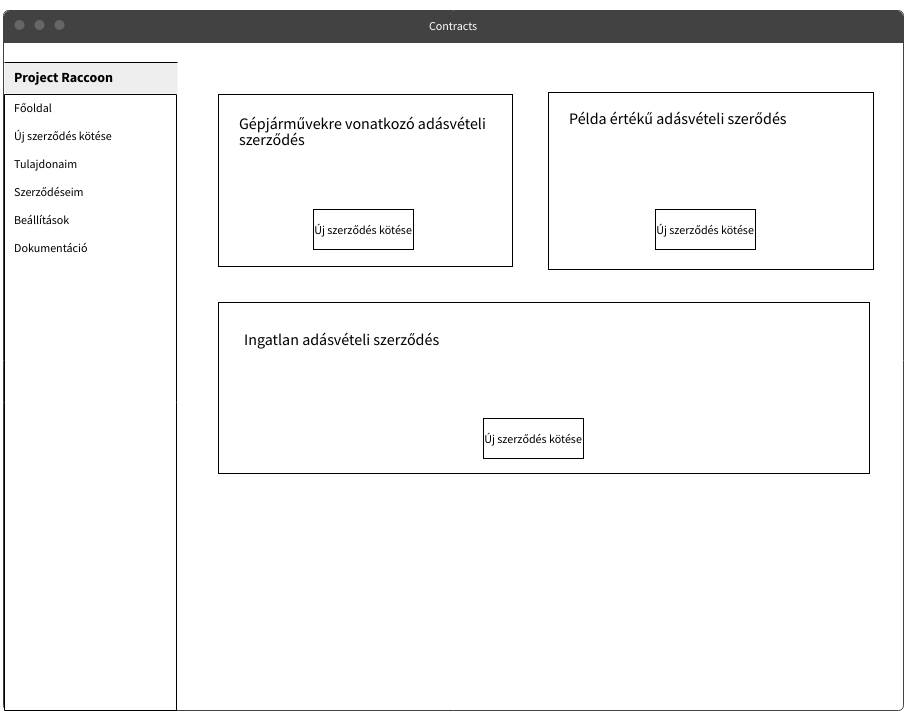
\includegraphics[scale=0.5]{images/wireframe/contracts.png}
	\caption{A Project Raccoon szerződéseket listázó felületének drótváza}
        \label{wireframe:contracts}
\end{figure}

Az eddigi példákból látható, hogy a tervezést a minél egyszerűbb használat, a letisztult design valamint a hatékony haszálhatóság vezérelte. A következő, \ref{chapter4}. fejezetben részletesebben kitértünk a megvalósítás részleteire, a felületek megvalósítására.

\section{Felhasználói use case-ek}

\begin{figure}[!h]
	\centering
        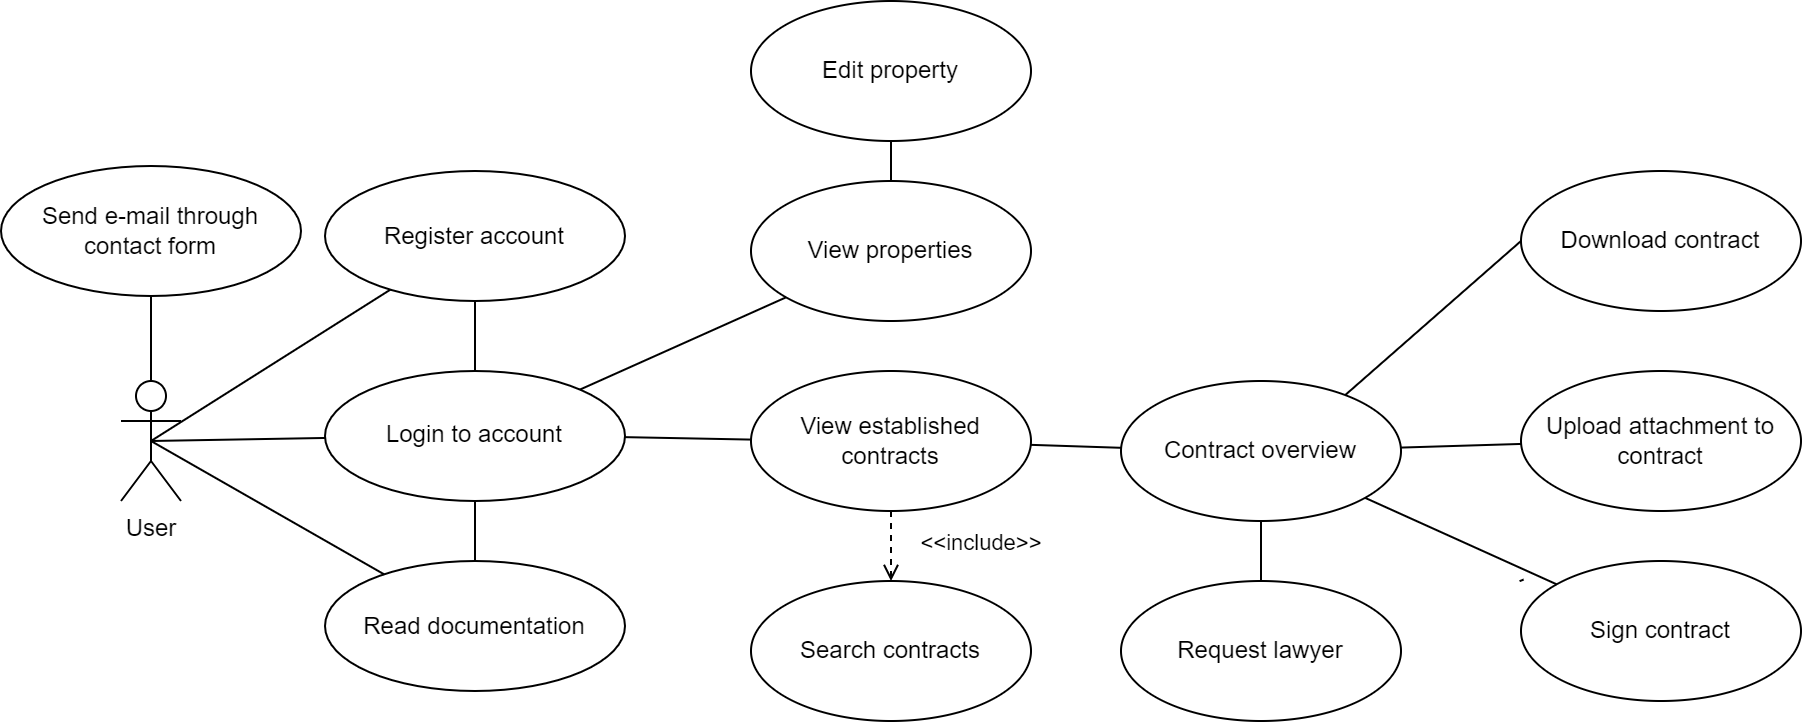
\includegraphics[scale=0.25]{images/software/user-use-case.png}
	\caption{A hitelesített felhasználók use case diagramja}
        \label{software:userusecase}
\end{figure}

A \ref{software:userusecase}. ábrán látható az összes funkcionalitás, amelyre jogosultak a felhasználók. Mivel nagyon sok funkcionalitás van, az ábrán egy leegyszerűsített diagram látható. Kezdeti fázisban, mikor a felhasználó a főoldalon van, küldhet egy e-mail-t a weboldal adminisztrátorainak egy kapcsolatfelvételi űrlapon keresztül, készíthet egy saját fiókot, beléphet egy már létező fiókba, vagy megtekintheti a felhasználók számára készített kézikönyvet.

A belépés után a felhasználók megnézhetik a meglévő szerződéseiket vagy megtekinthetik a saját tulajdonaikat. A saját tulajdonaik megtekintése közben az egyes tulajdonokat szerkeszteni is tudják. A szerződések megtekintése közben kereshetnek a szerződések között, vagy akár megtekinthetnek egy meglevő szerződést.

A meglévő szerződések megtekintése során a felhasználók kérhetnek ügyvédet a szerződés ellenőrzésére, letölthetik a szerződést, amennyiben mindenki aláírta, feltölthetnek mellékleteket egy nem véglegesített szerződés keretén belül, vagy aláírhatják a szerződést.

A \ref{software:contractdownload}. táblázatban az egyik legfontosabb use case: a szerződések letöltésének kiterjesztett magyarázatát láthatjuk.

\begin{longtable}{|p{0.35\textwidth}|p{0.55\textwidth}|}
\caption{Felhasználási eset: Szerződés letöltése}
\label{software:contractdownload}
\hline
\multicolumn{2}{|c|}{\textbf{Felhasználási eset}} \\
\hline
\textbf{Felhasznási eset száma:} & PR-1 \\
\hline
\textbf{Felhasznási eset leírása:} & Egy felhasználó letölti az egyik szerződése véglegesített, kitöltött PDF verzióját. \\
\hline
\textbf{Előfeltételek:} & 
\begin{enumerate}[itemsep=0pt,parsep=0pt,topsep=0pt,partopsep=0pt]
    \item A felhasználónak be kell jelentkeznie.
    \item A szerződés összes  kell lennie.
    \item A szerződést minden félnek alá kell írnia, beleértve az ügyvédeknek is.
    \item A felhasználónak hozzáférése kell legyen a szerződéshez.
\end{enumerate} \\
\hline
\textbf{Alapfolyamat:} & 
\begin{enumerate}[itemsep=0pt,parsep=0pt,topsep=0pt,partopsep=0pt]
    \item A felhasználó bejelentkezik a kezelőfelületre.
    \item A felhasználó listázza az összes szerződését, majd a kívánt szerződésre kattint, legyen az manuális kereséssel vagy a "Szerződések keresése" felhasználási esettel.
    \item A felhasználó rákattint a "Szerződés letöltése" gombra.
    \item A szerződés letöltődik a felhasználó számítógépére PDF fájlként.
\end{enumerate} \\
\hline
\end{longtable}

\begin{figure}[!h]
	\centering
        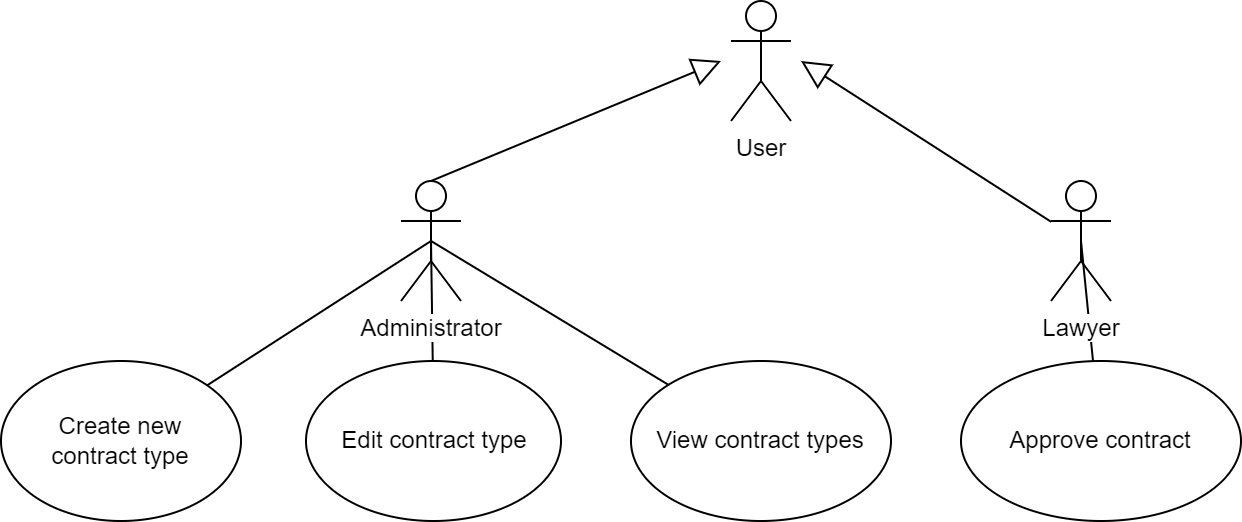
\includegraphics[scale=0.33]{images/software/special-use-case.png}
	\caption{A speciális felhasználók use case diagramja}
        \label{software:specialusecase}
\end{figure}

A \ref{software:specialusecase}. ábrán látható a speciális felhasználók számára elérhető funkcionalitások. Mivel az adminisztrátorok és az ügyvédek egyaránt felhasználók, mindenre képesek, amire a rendes felhasználók is képesek.

Az ügyvéd felhasználók alá tudják írni azokat a szerződéseket, amelyre meghívták őket, illetve az adminisztrátorok képesek létrehozni új szerződés típusokat, ki tudják listázni és meg tudják módosítani egyenként őket.

\pagebreak
	\chapter{Kivitelezés} \label{chapter4}

Ahogy az elző fejezet végén tárgyaltuk a felületek létrehozásánál, az elsődleges szempont a könnyű kezelhetőség és átláthatóság volt. Ezt kiegészítette a felhasználók számára létrehozott Súgó opció is, amelyet a portál kézikönyvének is nevezehetünk - a felhasználók útbaigazítását, esetleges problémamegoldást biztosít egyéb külső segítség (ügyfélszolgálat) nélkül. Az \ref{chapter3}. fejezetben kifejtettük ennek egyre jelentősebb fontosságát.

\begin{figure}[!h]
	\centering
        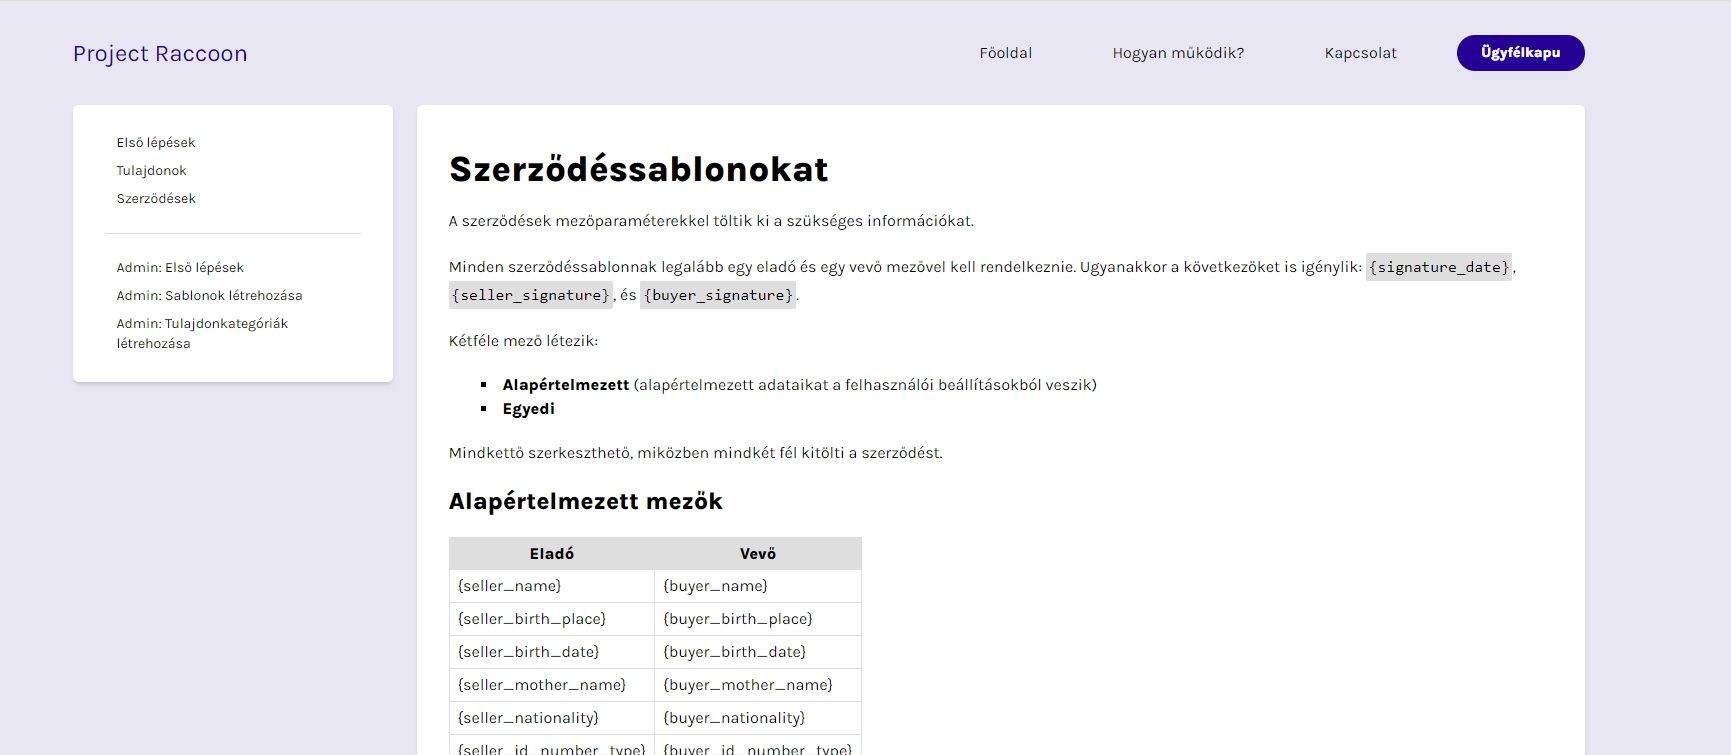
\includegraphics[scale=0.4]{images/design/admin-doc.png}
	\caption{A szerződéssablonok létrehozásának súgója}
        \label{design:adminDoc}
\end{figure}

A súgó, vagyis a menüben ``Dokumentáció''-ként megjelenő menüpont két részre osztódik. Létezik egy az átlagos felhasználók számára, és készült egy az adminisztrátorok számára is. Erre a döntésre azért jutottunk, mert nem szerettük volna az átlagos felhasználók számára is megjeleníteni olyan információkat, amelyeket nem tudnak elérni, tehát használhatatlan lett volna számukra. Így minden, amit megtalálnak a súgóban az releváns és naprakész marad számukra, nem árassza el őket a végtelen/szűretlen információk tárháza. A \ref{design:adminDoc}. ábrán láthatjuk az adminisztrátorok számára készült verzió egyik oldalát, pontosabban a szerződéssablonok létrehozását és magyarázatát. Ezzel kanyarodjuk is át egy fontos témakörhöz, mégpedig ahhoz, hogyan kezeli a Raccoon, és pontosabban hogyan adhatunk hozzá mi szerződéssablonokat, mint adminisztrátorok a portálon. 

A szerződéssablonok feltölthetőek az ``Új szerződés létrehozása'' menüpont alatt (amely megtalálható a navigációs menü admin részén, közvetlenül az előző fejezetben tárgyalt menüpontok alatt). A szerződések mezőparaméterekkel töltik ki a szükséges információkat. Minden szerződéssablonnak legalább egy eladó és egy vevő mezővel kell rendelkeznie. Ugyanakkor a következőket is igénylik: \verb|{signature_date}|, \verb|{seller_signature}|, és \verb|{buyer_signature}|. Kétféle mező létezik:
\begin{itemize}
    \item Alapértelmezett mező (alapértelmezett adataikat a felhasználói beállításokból veszik)
    \item Egyedi mező
\end{itemize}

Alapértelemett mező esetén a következőekre kell gondolni: a vevő, illetve eladó neve, email címe, telefonszáma, személyi igazolvány típusa és száma, születési helyük és idejük stb. A \verb|{signature_date}| egy speciális mező, amely tartalmazza azt a dátumot, amikor a szerződést mindkét fél aláírta. A \verb|{seller_signature}| és a \verb|{buyer_signature}| helyére mind az eladó, mind a vevő neve nagybetűvel kerül. 

Egyedi mezők megadására is lehetőség van, ekkor ezeknek meg kell adni típusát, beírható karakterek hosszát és egyéb esetleges megkötéseket stb a második fázisban. 

A \ref{exampleContract}. ábrán láthatunk egy ilyen példa szerződést, hogy hogyan is nézne ki a mezőkkel.

\begin{figure}[!h]
	\centering
        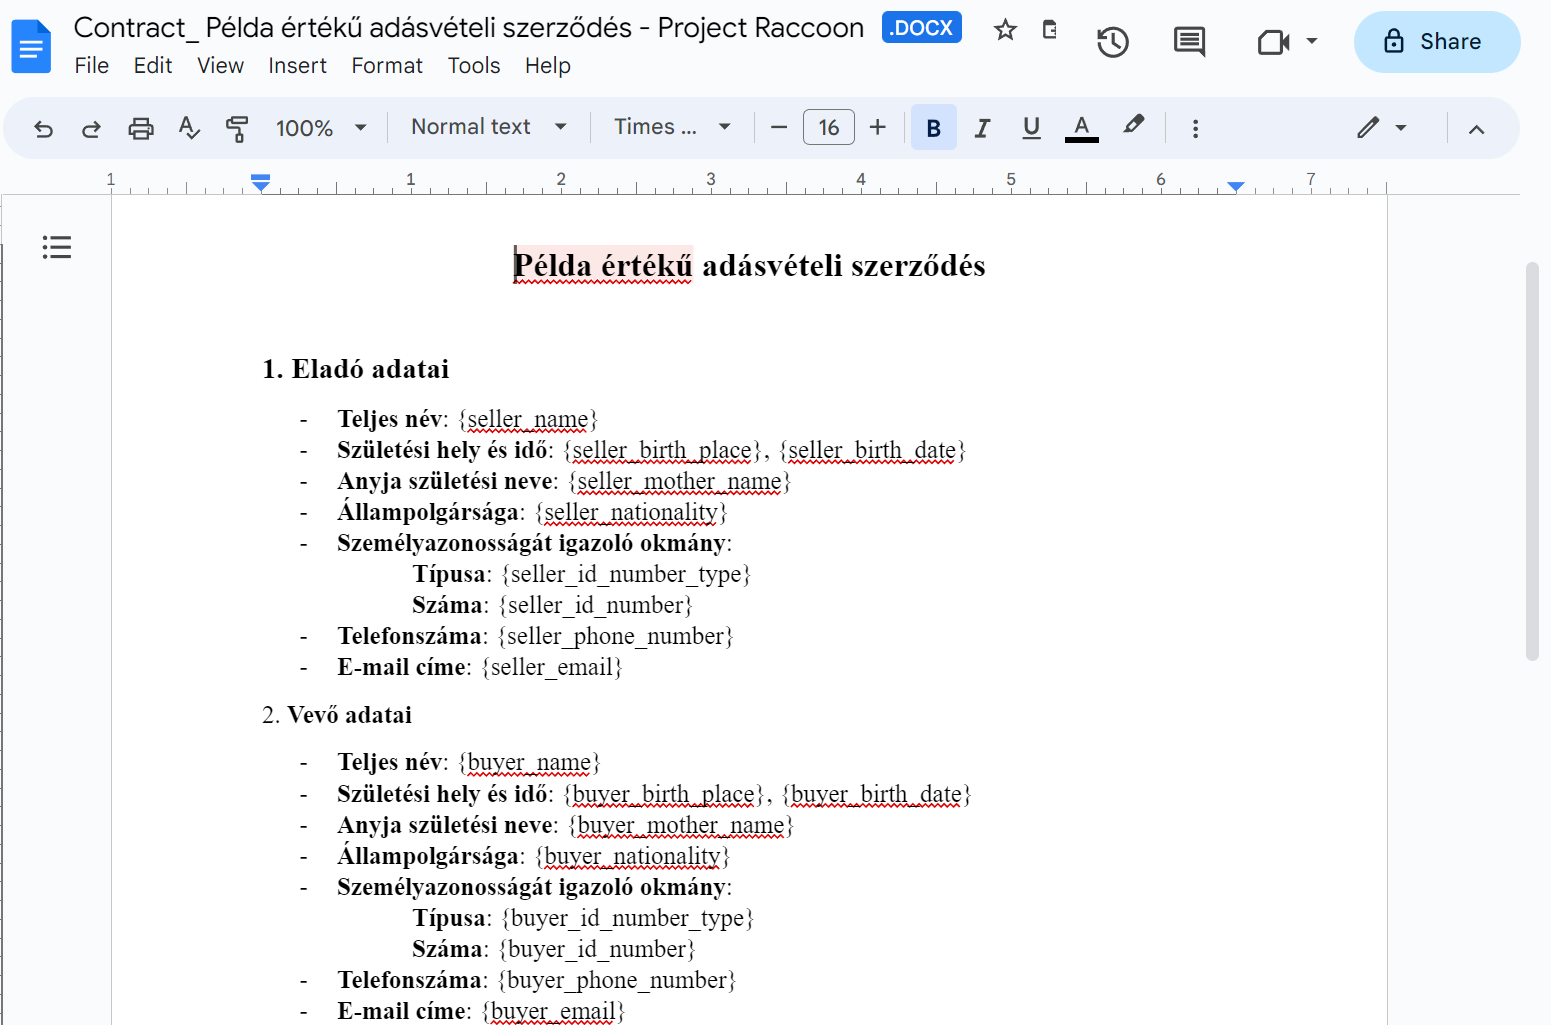
\includegraphics[scale=0.4]{images/design/google-docs.png}
	\caption{Példa értékű adásviteli szerződés szerkesztése Google Docsszal}
        \label{exampleContract}
\end{figure}

Ezen sablondokumentumok szerkeszthetőek Google Docs segítségével, illetve új sablonokat is fel lehet tölteni. 

Egy tényleges új sablon bevezetéséhez szükséges a továbbiakban a platformon megadni a helyettesítési mezőket és azok ``értékeit''. Vagyis miután feltöltöttük a sablont, amely tartalmazza a cserélendő szövegeket a következő formában: \verb|{replacement_option}|, az adminisztrátornak meg kell mondania, hogy ezeket a \{\} közé írt szövegeket a Raccoon mivel helyettesítse. Illetve itt történik a különböző megkötések megadása is, amelyek ezekre a mezőkre érvényesek kell legyenek. 

Összefoglalva tehát a folyamat két lépésből áll: 
\begin{enumerate}
    \item sablon készítése Google Docs-on
    \item helyettesítési mezők megadása a Raccoonon
\end{enumerate}

\begin{figure}[!h]
	\centering
        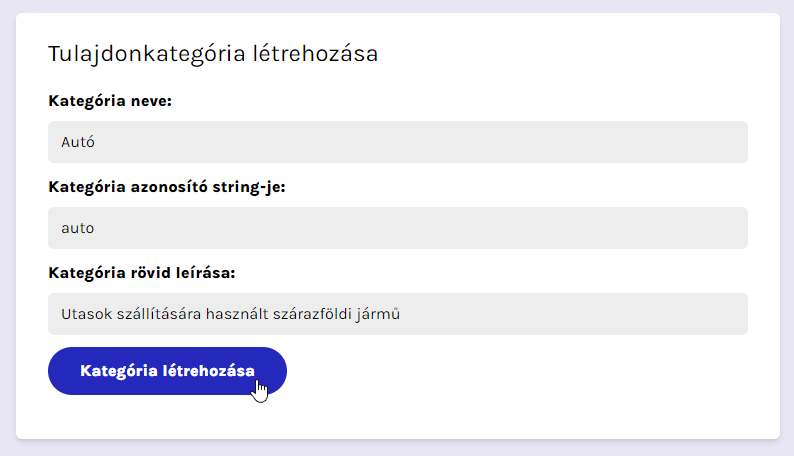
\includegraphics[scale=0.4]{images/design/new-property-category.png}
	\caption{Egy új tulajdonkategória (autó) hozzáadása a Raccoon platformján}
        \label{design:newPropertyCategory}
\end{figure}

Hasonlóképp létrehozhatóak új tulajdonkategóriák is (\ref{design:newPropertyCategory}. ábra). Ebben az esetben egy űrlapot kell kitölteni a Raccoon platformján. Új tulajdonkategória létrehozásához meg kell adnia egy nevet és egy rövid leírást. A kategória azonosítója automatikusan kitöltődik a kategória neve alapján, de szerkeszthető. Az összes korábban létrehozott kategóriát megtekinthetjük a ``Tulajdonkategóriák'' menüpont alatt. Új mezőt is hozzáadhatunk egy meglévő tulajdonkategóriához, ehhez az előbb említett menüben ki kell választani egy, majd megnyomva a ``Kategória szerkesztése'' gombot elénk tárul egy menü, ahol új mezőket adhatunk hozzá a kiválasztott tulajdonkategóriához. A következő paramétereket tudjuk megadni egy ilyen mezőnek: a típusa, prioritása (magasabb prioritás hamarabb jelenik meg), neve, egy hosszabb leírás/magyarázat (nem kötelező), sugó szöveg (nem kötelező), helyettesítő karakterlánc a dokumentumban (ennek a mezőnek a .docx sablonban is szerepelnie kell), minimális hossz (megkötés, nem kötelező), illetve maximális hossz (megkötés, szintén nem kötelező). Ha a hossz helyére $-1$-et írunk, az azt jelenti, hogy a hossz nincs meghatározva. A \ref{design:newPropertyField}. ábrán egy ilyen űrlapot töltöttünk ki egy új mező létrehozására.

\begin{figure}[!h]
	\centering
        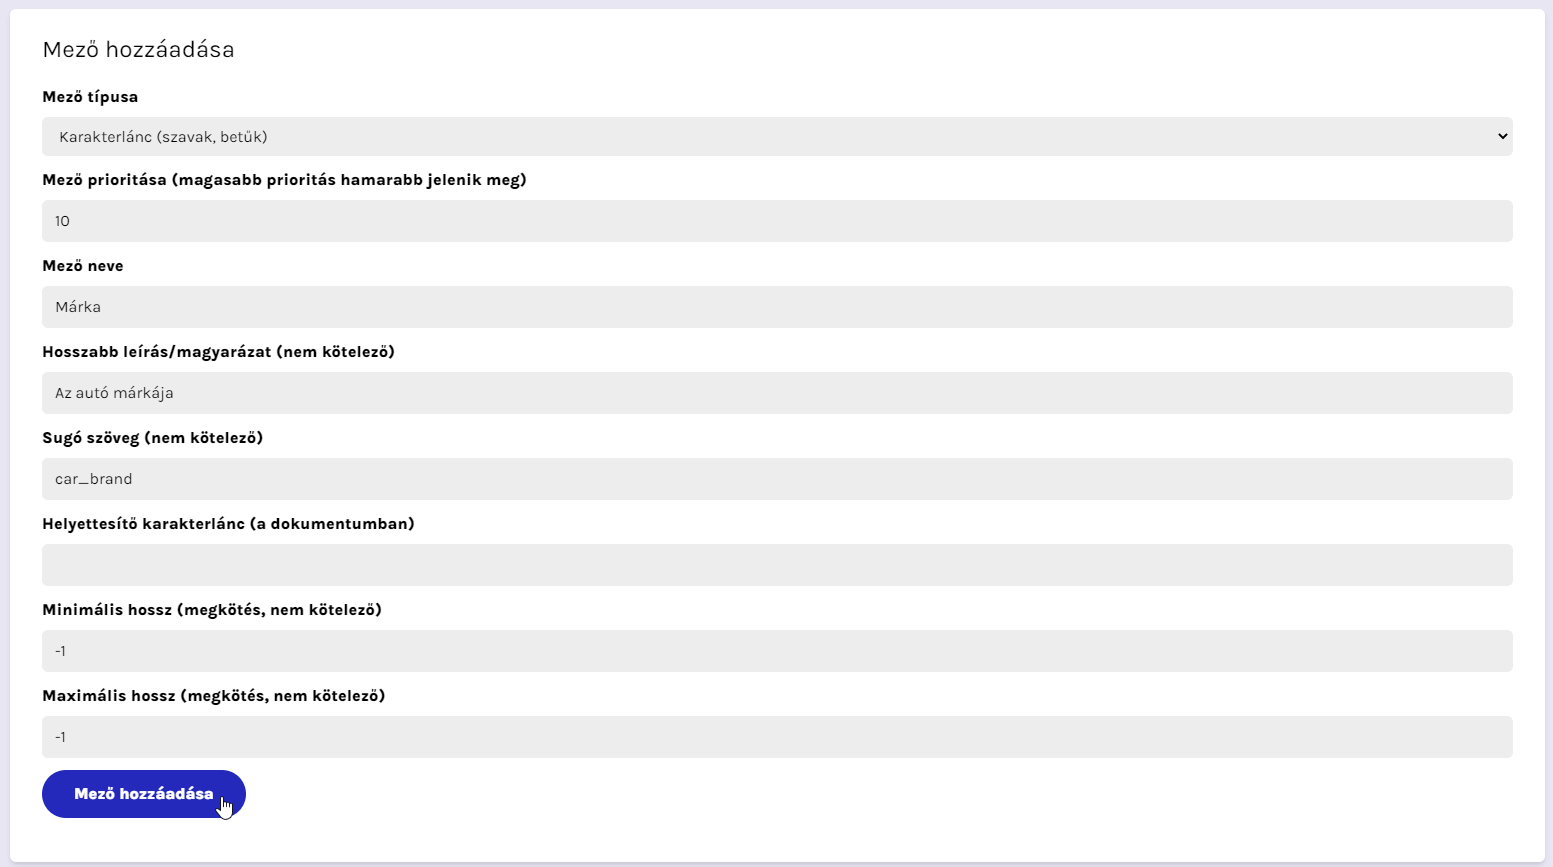
\includegraphics[scale=0.36]{images/design/new-property-field.png}
	\caption{Egy új mező (márka) hozzáadása a Raccoon platformján}
        \label{design:newPropertyField}
\end{figure}

A szerződésekhez lehet ügyvédeket is hozzáadni, az ``Ügyvéd hozzáadása'' menüpont alatt, amely email cím alapján történik. Ezt szintén csak adminisztrátori jogkörrel lehetséges. 

Az átlagfelhasználó számára rendkívül fontos, hogy könnyen áttekinthető módon kezelje szerződéseit és tulajdonait. Az alkalmazás lehetővé teszi számára, hogy listázza az összes szerződését és tulajdonát, amelyekben könnyedén kereshet név vagy típus alapján. 

Az alkalmazás továbbfejlesztésével lehetőséget adhatunk az átlagfelhasználónak arra is, hogy új szerződéseket vigyen be a rendszerbe. Ezáltal egyszerűen rögzítheti és kezelheti új üzleti vagy személyes szerződéseit a platformon keresztül. Az új szerződések felvitelekor a felhasználó részletes információkat adhat meg, például a szerződés leírását, a felek nevét és az érvényességi időtartamot. Ez segíti az átlagfelhasználót abban, hogy a szerződések könnyen azonosíthatók és kezelhetők legyenek.

Az aláírás és letöltés funkció nagyban megkönnyíti az átlagfelhasználó életét. Az alkalmazás lehetővé teszi, hogy a felhasználók elektronikusan aláírják a szerződéseket, így elkerülve a hagyományos papíralapú eljárásokat és a helyhez kötöttséget. Az aláírás után a felhasználók letölthetik a szerződéseket PDF formátumban, így könnyedén megőrizhetik és megoszthatják őket más féllel.

\begin{figure}[!h]
	\centering
        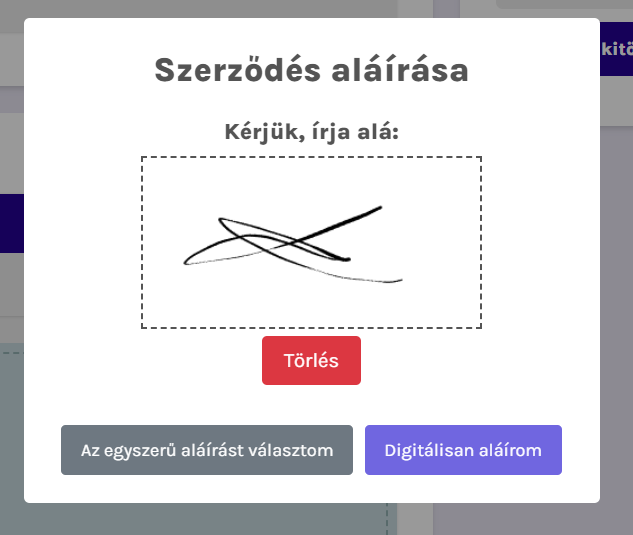
\includegraphics[scale=0.5]{images/design/signature.png}
	\caption{A szerződés digitálisan való aláírásra felhívó ablak}
        \label{design:signature}
\end{figure}

A szerződések aláírása digitális formában történik, erre lehetőséget ad a platform is. Az aláírásra való felkérést a \ref{design:signature}. ábra szemlélteti.

A felhasználók képesek a szerződések mellé csatolmányokat is feltölteni. Erre kényelmes megoldást biztosít az alkalmazás drag-and-drop formájában. Illetve, a felületre rákattintva az operációs rendszer fájlkiválasztó ablakát is megjeleníti. Ez látható a \ref{design:attachment}. ábrán. Abban az esetben, hogyha a felhasználó nem szeretné digitálisan aláírni a szerződést, kiválaszthatja a másik opciót is: az egyszerű aláírás lehetőségét. Az egyszerű aláírás segítségével nem kerül rá konkretán a szerződésre a felhasználó kézírása, helyette a felhasználó neve jelenik meg.

\begin{figure}[!h]
	\centering
        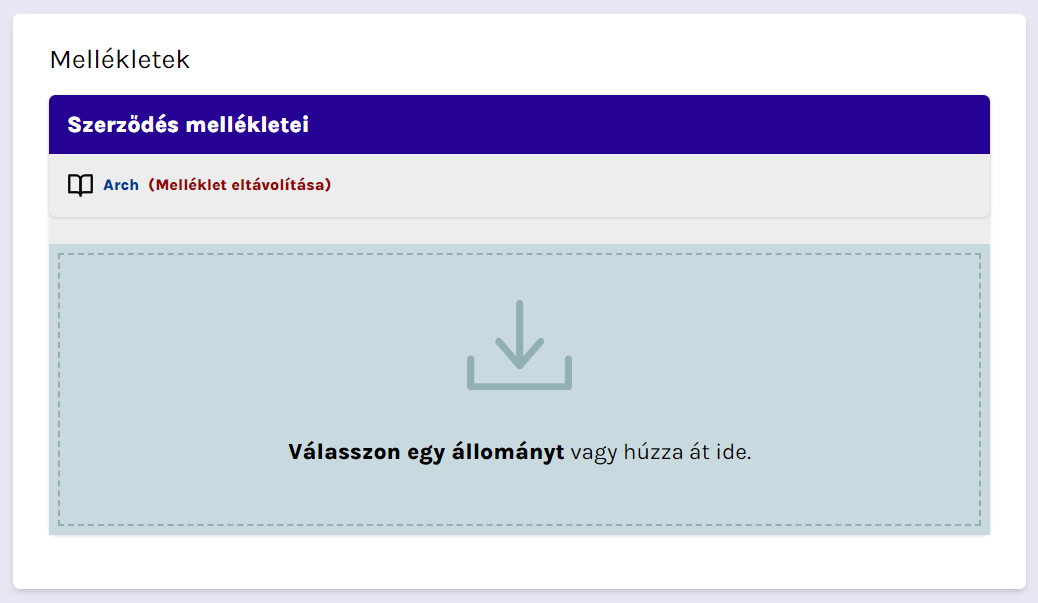
\includegraphics[scale=0.5]{images/design/attachment.png}
	\caption{A szerződésekhez különböző csatolmányokat lehet hozzáadni}
        \label{design:attachment}
\end{figure}

Ezek a fejlesztések hozzájárulnak az alkalmazás hatékonyságához és felhasználóbarát jellegéhez, lehetővé téve az átlagfelhasználó számára, hogy egyszerűen kezelje, keresse és aláírja a szerződéseit, valamint megőrizze fontos tulajdonainak nyilvántartását egy helyen.

Végezetül pedig a weboldalt elláttuk többnyelvűsítéssel is, így a felhasználók könnyedén válthatnak a különböző nyelvek között egy egyszerű kattintással. Ez lehetővé teszi, hogy az alkalmazás használata még inkább személyre szabható legyen, és a felhasználók anyanyelvükön vagy preferált nyelvükön használhassák azt. 

Emellett a platform elérhetővé tette a sötét téma opciót is. Ez lehetővé teszi a felhasználóknak, hogy a hagyományos világos háttér helyett a sötét témát válasszák, ami kevésbé megterhelő a szemüknek és energiatakarékosabb lehet, különösen alacsony fényviszonyok esetén.

Ezek az újítások további funkcionalitást és kényelmet biztosítanak az felhasználók számára, lehetővé téve számukra, hogy könnyedén váltogassanak nyelvek között, és kiválasszák az optimális megjelenést a számukra. Az alkalmazásunk így még rugalmasabbá válik, és az egyéni preferenciákhoz igazodva személyre szabott felhasználói élményt nyújt.
	\chapter{Mérések} \label{chapter5}

A webes alkalmazások kitelepítése hagyományosan szerverek felállításával, bekonfigurálásával és kezelésével járt, viszont a felhőalapú technológiák rohamos fejlődése egy alternatív megközelítést vezetett be: a \textit{serverless} megközelítéseket. Ennek a fejezetnek az a célja, hogy összehasonlítsa a \textit{serverless} telepítések teljesítmény- és költségmetrikáit a hagyományos szerver telepítésekével. 

A vizsgálat megvalósítása érdekében a \textit{Project Raccoon}-nak két változatát hoztuk létre: az egyiket Docker segítségével telepítettük ki, ami a hagyományos szerveres megközelítést képviseli, a másikat pedig \textit{serverless} technológiák segítségével, konkrétan a Vercel használatával.

A teljesítménymutatók, például a válaszidők, az erőforrás-kihasználás, valamint a költségmutatók körbejárásával a fejezet célja, hogy rávilágítson ezeknek a telepítési stratégiáknak az előnyeire és korlátaira.

Olyan információkat szeretnénk mutatni, melyek informálhatják a döntéshozatali folyamatot a fejlesztők számára a kitelepítést illetően.

Az összés mérést Marosvásárhelyen készítettük, egy AMD Ryzen 5 5600H-es számítógépen, 16 GB memóriával és 1000 megabites hálózati sávszélességgel. A hagyományos szerver Németországban van kitelepítve a Hetzner szolgáltatónál: egy CPX11 szerverről van szó.

A Docker-es megvalósítás elérhető a következő linken, illetve letölthető a diplomadolgozat mellékleteiből is: \url{https://raccoon.tohka.us}

A Vercel-es (\textit{serverless}) megvalósítás elérhető a következő linken: \url{https://raccoon.sallai.me}

\pagebreak

\section{Késleltetési teszt: hidegindítás esetén}

\begin{figure}[!h]
	\centering
        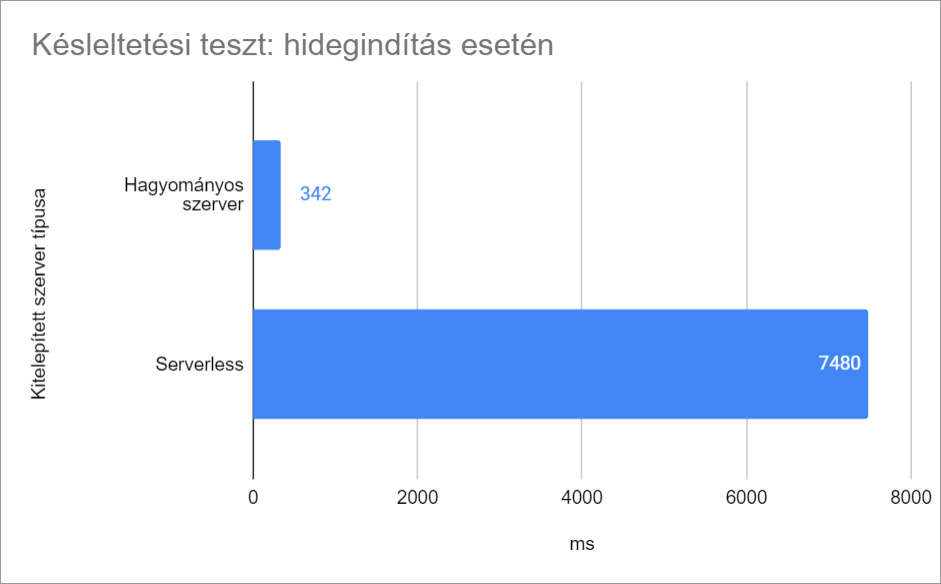
\includegraphics[scale=0.75]{images/measurement/diagram1.png}
	\caption{Késleltetési teszt: hidegindítás esetén}
        \label{measure:diagram1}
\end{figure}

A \ref{measure:diagram1}. ábrán látható a késleltetési teszt eredményei hidegindítás esetén. A tesztet 10-szer hajtottuk végre. A teszt során egy Python program segítségével lemértük, mennyi időbe kerül, hogy válaszoljon a weboldal. Az eredményeket átlagoltuk. A futtatások között vártunk 10 percet, annak érdekében, hogy a serverless környezetben futtatott alkalmazás kikerüljön a meleg futtatási környezetéből.

Látható, hogy a serverless weboldalnak jelentősen több időbe kerül válaszolnia a hidegindítás során a kérésekre. Ez azzal magyarázható, hogy a felhőben a szerver le kell töltse a futtatás előtt a futtatandó függvényeket. Ha fontos, hogy mindig egyből elérhető legyen az alkalmazásunk, válasszuk a hagyományos szervert.

\pagebreak

\section{Késleltetési teszt: melegindítás esetén}

\begin{figure}[!h]
	\centering
        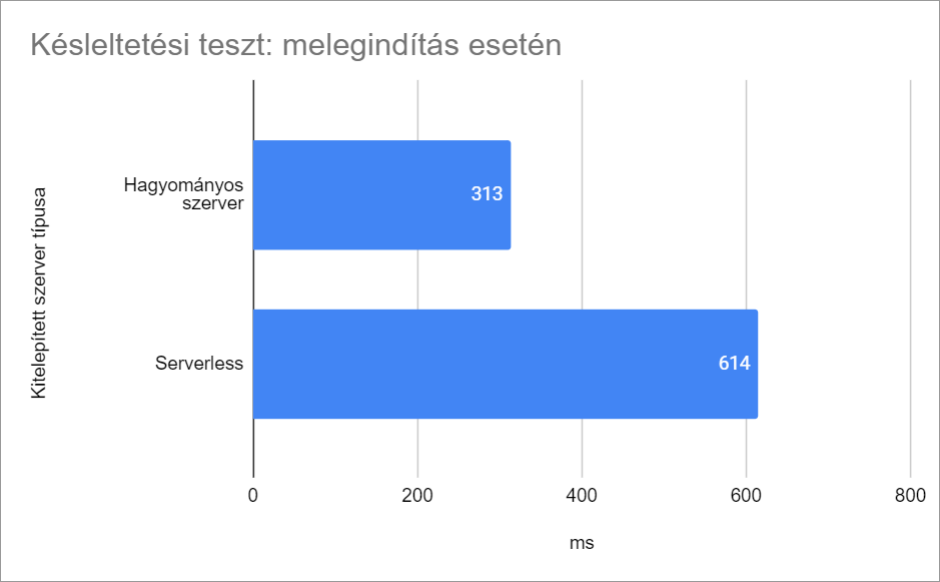
\includegraphics[scale=0.75]{images/measurement/diagram2.png}
	\caption{Késleltetési teszt: melegindítás esetén}
        \label{measure:diagram2}
\end{figure}

A \ref{measure:diagram2}. ábrán látható a késleltetési teszt eredményei melegindítás esetén. Hasonlóképpen az előző tesztet, egy Python program segítségével lemértük, hogy mennyi időbe kerül az alkalmazás válasza a kéréseinkre. A weboldal főlapját kértük el, hitelesítés nélkül. A tesztet 100-szor futtattuk le, egymás után, várakozás nélkül. Az első 5 eredményt elvetettük, a többit átlagoltuk.

Ha összehasonlítjuk az eredményeket a \ref{measure:diagram1}. 
ábrával, észrevehetjük, hogy nem létezik különösebb különbség a késleltetés szempontjából a meleg és hideg indítások során a hagyományos szervereknél.

A \ref{measure:diagram2} ábrát nézve megfigyelhetjük, hogy bár a hagyományos szerver Németországban van kitelepítve, a hagyományos szerver kevesebb késleltetésben szenved mint a serverless megoldás. 

\pagebreak

\section{Telepítési idő frissítéskor}

\begin{figure}[!h]
	\centering
        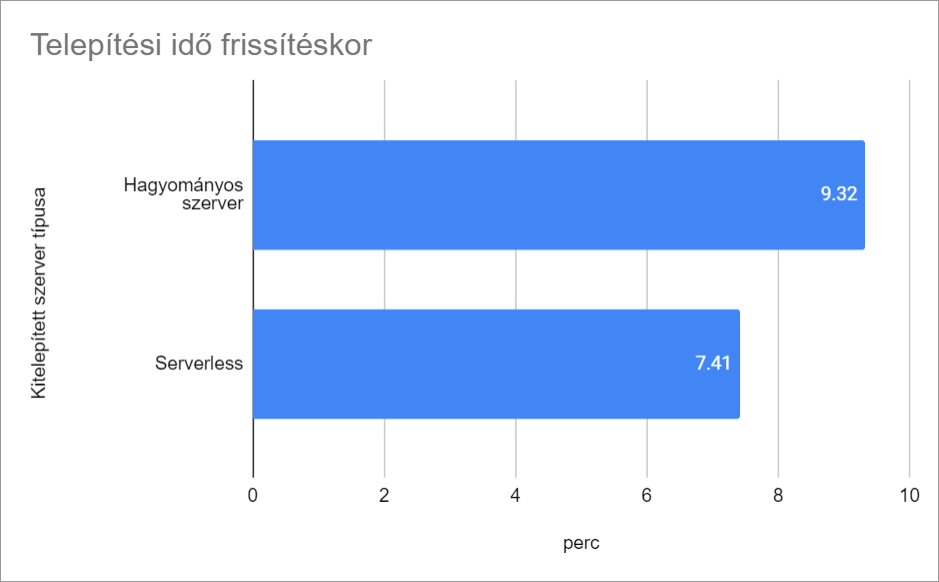
\includegraphics[scale=0.75]{images/measurement/diagram3.png}
	\caption{Telepítési idő frissítéskor}
        \label{measure:diagram3}
\end{figure}

A \ref{measure:diagram3}. ábrán látható a telepítési teszt eredményei frissítéskor. A Vercel platformról a legutolsó 5 telepítés idejét vettük a serverless adatoknak, míg a hagyományos szerverek esetében lefuttattuk ötször a Docker buildelési és telepítési folyamatát. A telepítési időket átlagoltuk.

A serverless platform majdnem két egész perccel gyorsabb a hagyományos szervernél. A hagyományos szerver telepítésének lassúsága magyarázható azzal, hogy a Hetzneres szerver, amelyre telepítettük a rendszert, csupán egy CPX11 instance: két CPU core-al rendelkezik, ami nem segíti elő egyáltalán a párhuzamos telepítési folyamatot.

Ha gyorsabb telepítést szeretnénk, akkor mindenképp válasszunk serverless megoldást.

\pagebreak

\section{Költségelemzés havonta: alacsony használati előrejelzés}

\begin{figure}[!h]
	\centering
        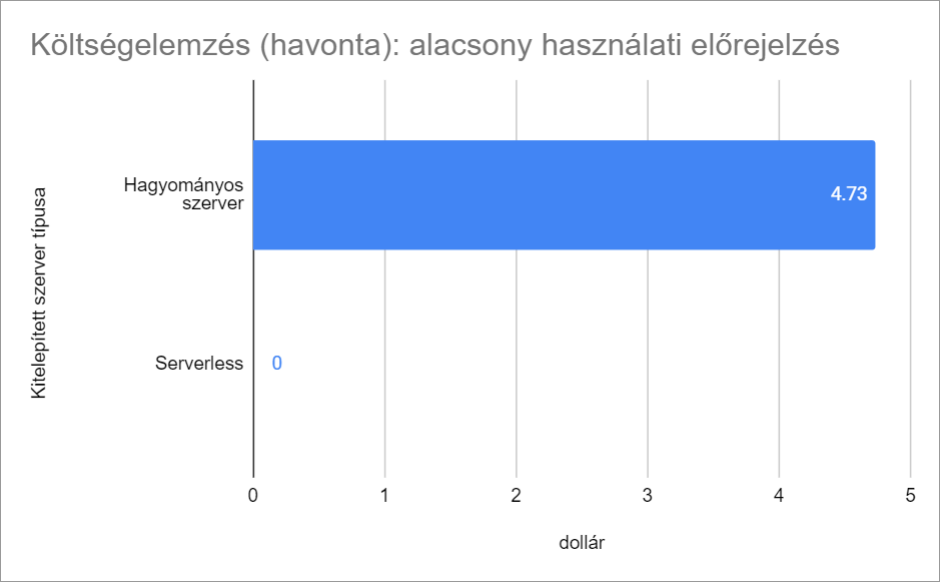
\includegraphics[scale=0.75]{images/measurement/diagram4.png}
	\caption{Költségelemzés havonta: alacsony használati előrejelzés}
        \label{measure:diagram4}
\end{figure}

A \ref{measure:diagram4}. ábrán látható a költségelemzés alacsony használati előrejelzésre. A költségelemzésünk egyszerű volt ebben az esetben: a hagyományos szervernek egy Hetzner CPX11 szervert választottunk, míg a serverless megoldásnak a Vercel ingyenes \textit{free tierjét} választottuk.

Mivel a Vercel teljesen ingyenesen használható 500,000 kérésig, ezért alacsony használat esetében teljesen ingyenes. A hagyományos szerver futtatása viszont pénzbe kerül: pontosan 4.73 dollárba. Ha nagyon kevés felhasználónk van, nincs értelme egy egész szervert kibérelni.

\pagebreak

\section{Költségelemzés havonta: magas használati előrejelzés}

\begin{figure}[!h]
	\centering
        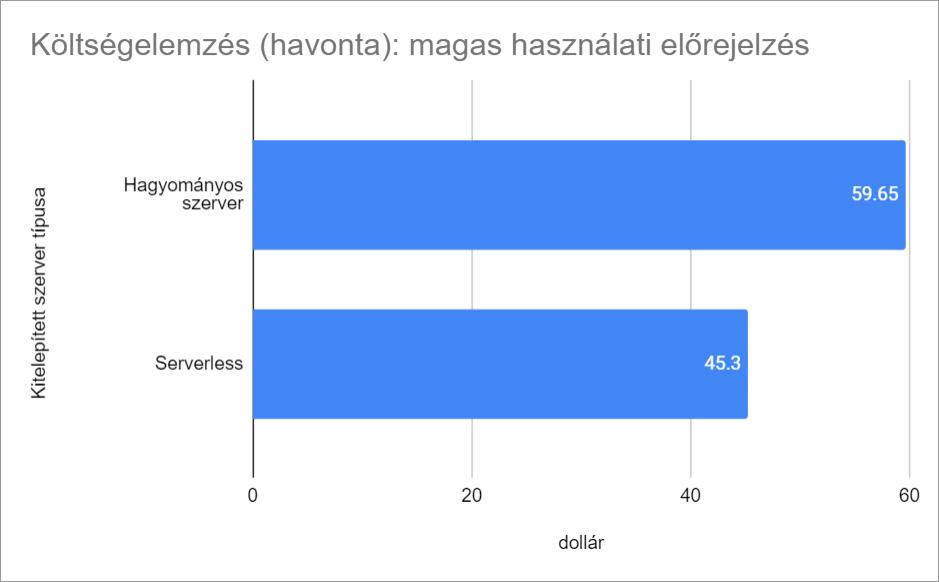
\includegraphics[scale=0.75]{images/measurement/diagram5.png}
	\caption{Költségelemzés havonta: magas használati előrejelzés}
        \label{measure:diagram5}
\end{figure}

A \ref{measure:diagram5}. ábrán látható a költségelemzés magas használati előrejelzésre.  A költségelemzésünk itt már komplikáltabb. Hagyományos szervernek a Hetzner CPX51 szerverét választottuk. Ennek költségét nagyon könnyű kiszámítani – egyetlen összetevőről van szó.

Serverless kontextusban sokkal bonyolultabbak a számítások. A serverless világban kell fizetni a programozók számáért is, a kérések számáért, illetve a sávszélességért is. 3 millió kérésben gondolkodtunk, 2 programozóban és 1 terabyte sávszélességben. Mivel egy felhasználó 20 dollárba kerül havonta, illetve 1 millió után minden millió kérés után 2.65 dollárt kér a Vercel, ezért a végeredmény 59.65 dollár.

Ha nem szeretnénk túlkomplikálni az életünket hasonló számítgatásokkal, jobban megéri a hagyományos szerver, amelynek futtatási költségei mindig konstansak maradnak.
	%----------------------------------------------------------------------------
\chapter*{Összefoglaló}\addcontentsline{toc}{chapter}{Összefoglaló}
%----------------------------------------------------------------------------

A felgyorsult digitalizáció rengeteg újítást hoz a modern ember életében, beszivárog a mindennapjainka, legyen szó munkahelyről, oktatásról vagy épp egyéb területről. 

A Project Raccoon a digitalizáció által nyújtott lehetőségeket kihasználva továbbfejleszti az ügyintézési folyamatokat, segítve ezzel a modern ember mindennapjait. A platform rugalmas és felhasználóbarát felülete révén könnyen kezelhető, és a felhasználók számára egyszerűbbé teszi az adminisztratív feladatokat.

Ez a rendszer számos előnyt kínál a felhasználók számára, akik így időt és erőforrásokat takaríthatnak meg azáltal, hogy a hagyományos papíralapú folyamatokat digitális formába helyezik át. Segítségével az emberek könnyedén intézhetik ügyeiket otthonról, anélkül, hogy személyesen kellene felkeresniük különböző hivatalokat vagy intézményeket. Az online felületen elérhetővé válnak az igazolások, űrlapok, dokumentumok, amelyeket könnyedén kitölthetnek. Ezenkívül a platform lehetővé teszi a dokumentumok elektronikus aláírását, amely hitelesített módon helyettesíti a hagyományos, papíralapú aláírást. Ezáltal a felhasználók biztonságosan és megbízhatóan intézhetik ügyeiket az online térben.

A mérésekből bebizonyosodott, hogy mind a hagyományos szerver alapú kitelepítéseknek, mind a \textit{serverless} technológiákkal kitelepített környezeteknek még mindig van létjogosultságuk. Attól függően, hogy mekkora projektet készítünk, és milyen gyakran fogják használni a felhasználók, kell döntenünk a hasonló telepítési kérdésekről.

\hiddensubsection{GitHub projekt linkje}

A projekt forráskódja elérhetően a következő linken: \url{https://github.com/darktohka/project-raccoon}.

% Koszonetnyilvanitas
%~~~~~~~~~~~~~~~~~~~~~~~~~~~~~~~~~~~~~~~~~~~~~~~~~~~~~~~~~~~~~~~~~~~~~~~~~~~~~~~~~~~~~~
%	\include{acknowledgement}


% Tablazatok es abrak jegyzeke (EZ NEM KOTELEZO)
%~~~~~~~~~~~~~~~~~~~~~~~~~~~~~~~~~~~~~~~~~~~~~~~~~~~~~~~~~~~~~~~~~~~~~~~~~~~~~~~~~~~~~~
	\listoffigures\addcontentsline{toc}{chapter}{\abrakjegyzeke}
	\listoftables\addcontentsline{toc}{chapter}{\tablazatokjegyzeke}


% Bibliography
%~~~~~~~~~~~~~~~~~~~~~~~~~~~~~~~~~~~~~~~~~~~~~~~~~~~~~~~~~~~~~~~~~~~~~~~~~~~~~~~~~~~~~~
	\bibliography{bibliography}
	\addcontentsline{toc}{chapter}{\irodalomjegyzek}
	\bibliographystyle{ieeetr}
	
% Appendix
%~~~~~~~~~~~~~~~~~~~~~~~~~~~~~~~~~~~~~~~~~~~~~~~~~~~~~~~~~~~~~~~~~~~~~~~~~~~~~~~~~~~~~~
%	\include{appendices}

\label{page:last}
\end{document}
